%% Latex template for PhD dissertation or MS thesis
%% Department of Electrical and Computer Engineering
%% Brigham Young University
%% Last Modified: July 2017 by mdr@byu.edu

\documentclass[12pt,oneside]{report}
% generate the one-sided version: this is the ETD version
% print the one-sided version one sided for all the department and college approvals

% \documentclass[12pt,twoside]{report}
% Uncomment this line (and comment line 6) to create the two-sided version.
% Print the two-sided version two-sided for the optional printed and bound version.

%%%%%%%%%%%%%%%%%%%%%%%%%%%%%%%%%%%%%%%%%%%%%%%%%%%%%%%%%
%  Setup BYU thesis format
%%%%%%%%%%%%%%%%%%%%%%%%%%%%%%%%%%%%%%%%%%%%%%%%%%%%%%%%%
\usepackage{byustyle}
% Setup the byu style sheet
\byustylesetup{%
    %
    isdissertation = false,            % false for MS thesis, true for PhD dissertation
	%
    % Definitions of names needed in thesis/dissertation
    deptname          = Department of Electrical and Computer Engineering,
    committeechairman = Randal W. Beard,
    committeemembera  = Timothy W. McLain,
    committeememberb  = Cameron K. Peterson,
	committeememberc  = Brad L. Hutchings, % needed for dissertation, ignored for thesis
	committeememberd  = Steven M. Schultz,    % needed for dissertation, ignored for thesis
    %
    %Change true/false to shorten for proofreading purposes
    noabstract = false,         % Do not show the abstract page
    nouniversitypages = false,  % Do not show any of the "university pages"
    noacknowledgements = false, % Do not show the Acknowledgements page
    notableofcontents = false,  % Do not show the Table of Contents
    nolistoffigures = false,    % Do not show the List of Figures
   	nolistoftables = false,     % Do not show the List of Tables
    nonomenclature = false,      % Do not show the Nomenclature section - note that this section is optional
    notocandlists = false,      % Do not show the Table of Contents, List of Figures, or the List of Tables
    noheaderatall = false,      % Do not show any of the BYU Thesis header pages
    keywords = {multi-agent, handoff, target, tracking, UAV} % your keywords
}

%%%%%%%%%%%%%%%%%%%%%%%%%%%%%%%%%%%%%%%%%%%%%%%%%%%%%%%%
% Package inclusions go here
% The list starts with some commonly used packages
% That do not conflict with byutyle.sty
%%%%%%%%%%%%%%%%%%%%%%%%%%%%%%%%%%%%%%%%%%%%%%%%%%%%%%%%


\usepackage{amssymb,amsmath}
\usepackage{amsfonts}
\let\saveboldmath\boldmath
\usepackage{mathptmx}
\let\boldmath\saveboldmath
\usepackage{bm}

\DeclareSymbolFont{cmsymbols}{OMS}{cmsy}{m}{n}
\SetSymbolFont{cmsymbols}{bold}{OMS}{cmsy}{b}{n}
\DeclareSymbolFontAlphabet{\mathcal}{cmsymbols}
\usepackage{graphicx}        			% for .pdf graphics inclusion
\usepackage[calcwidth = \columnwidth]{caption}
\usepackage{booktabs,threeparttable}
\usepackage{setspace}					%	change the spacing inside a document
\usepackage{epstopdf}					%	converts a .eps to a .pdf
\usepackage{cite}						%	allows for citations
\usepackage{float}						%	improves the interface for defining floating objects
\usepackage{rotating}
\usepackage{printlen}
\usepackage[table,xcdraw]{xcolor}


%%%%%%%%%%%%%%%%%%%%%%%%%%%%%%%%%%%%%%%%%%%%%%%%%%%%%%%%%%%%%%%%%%%%
%  Include additional \usepackage{} statements here.
%    Add one package at a time.
%    Warning:  Some packages are not compatible with byustyle.sty
%%%%%%%%%%%%%%%%%%%%%%%%%%%%%%%%%%%%%%%%%%%%%%%%%%%%%%%%%%%%%%%%%%%

%These next two lines are for the citing with the IEEE style
\renewcommand\citepunct{], [}
\renewcommand\citedash{]--[}

%%%%%%%%%%%%%%%%%%%%%%%%%%%%%%%%%%%%%%%%%%%%%%%%%%%%%%%%
% For doing bookmarks in the PDF file
%%%%%%%%%%%%%%%%%%%%%%%%%%%%%%%%%%%%%%%%%%%%%%%%%%%%%%%%%
% For more info, see:
% http://www.geocities.com/kijoo2000/latex2pdf.pdf
% http://www.tug.org/applications/hyperref/manual.html
\usepackage[pdftex,backref,pagebackref,plainpages=false]{hyperref}
\hypersetup{
    %bookmarks    = true, % Make bookmarks (default=true). This option
                          %cannot be used after package has been loaded,
                          %thus use like this: \usepackage[bookmarks=false]{hyperref}.
    %
    breaklinks   = false, % Allow link text to break across lines (default=false).
    linktocpage  = false, % make page number, not text, be link on TOC, LOF and LOT
    colorlinks   = false, % Color the text of links (true) or put color frames over
    %
    linkbordercolor  = {1 1 1}, % The color of the box around normal links (white so they won't show up)
    citebordercolor  = {1 1 1}, % The color of the box around citations (white so they won't show up)
                          % the links (false).
    pdfstartview = {FitV}, % Set the startup page view. Possible options are:
                           % FitH: Fit whole width of page
                           % FitV: Fit whole height of page
                           % FitB: Fit whole �Bounding Box� page
                           % FitBH: Fit whole width of �Bounding Box� of page
                           % FitBV: Fit whole height of �Bounding Box� of page
    bookmarksnumbered  = true, % Put section numbers in bookmarks (default=false)
    bookmarksopen      = true, % Open up the bookmark trees (default=false).
    bookmarksopenlevel = 0, % Level to which bookmarks are open (default=\maxdimen).
    bookmarkstype      = toc, % Specify which toc file to mimic (default=toc).
    pdfpagemode        = {UseOutlines}, %  Specify how document starts when opened ({None}).
                                        % Possible options are:,
                                        % None: Neither bookmarks nor thumbnails are visible.
                                        % UseOutlines: Bookmarks are visible.
                                        % UseThumbs: Thumbnails are visible.
                                        % FullScreen: Full-screen mode
    pdftitle    = {Thesis},
    pdftitle    = {First Line of your Thesis/Dissertation Title},
    pdfauthor   = {Isaac Newton},
    pdfcreator  = {Isaac Newton},
    pdfsubject  = {Isaac Newton's Master's Thesis},
    pdfkeywords = {Master's Thesis, BYU},
    pdfborder		=	{0 0 0},}

%%%%%%%%%%%%%%%%%%%%%%%%%%%%%%%%%%%%%%%%%%%%%%%%%%%%%%%%
%  Define macros here - You may use these, or delete them, as you see fit.
%%%%%%%%%%%%%%%%%%%%%%%%%%%%%%%%%%%%%%%%%%%%%%%%%%%%%%%%%

% % \def\proof{\noindent{\it Proof: }}
% % \def\QED{\mbox{\rule[0pt]{1.5ex}{1.5ex}}}
% % \def\endproof{\hspace*{\fill}~\QED\par\endtrivlist\unskip}
% % \newcommand{\norm}[1]{\left\|#1\right\|}
% \newcommand{\abs}[1]{\left|#1\right|}
% % \newcommand{\defeq}{\stackrel{\triangle}{=}}
% % \newcommand{\re}{\mathbb{R}} 		% real numbers
% % \newcommand{\OMIT}[1]{{}} 		% omit sections of text
% \newcommand{\pd}[2]{\ensuremath{\frac{\partial #1}{\partial #2}}} % partial derivative
% % \newcommand{\superscript}[1]{\ensuremath{^\textrm{#1}}}
% % \newcommand{\subscript}[1]{\ensuremath{_\textrm{#1}}}
\usepackage{algorithm}
\usepackage{algorithmicx}
\usepackage{algpseudocode}
\usepackage{mymacros}
\usepackage{import}


%%%%%%%%%%%%%%%%%%%%%%%%%%%%%%%%%%%%%%%%%%%%%%%%%%%%%%
% Define the 'inverted pyramid' table caption
% requirement from the College.
%%%%%%%%%%%%%%%%%%%%%%%%%%%%%%%%%%%%%%%%%%%%%%%%%%%%%%

\DeclareCaptionJustification{InvertedPyramid}{\hsize=\linewidth
                \parindent=0pt
                \leftskip=0pt plus.5fil
                \rightskip=0pt plus-0.5fil
                \parfillskip=0pt plus1fil
                \emergencystretch=1in
                \parshape10
                0.00in \linewidth
                0.025\linewidth 0.95\linewidth
                0.05\linewidth 0.9\linewidth
                0.075\linewidth 0.85\linewidth
                0.1\linewidth 0.8\linewidth
                0.125\linewidth 0.75\linewidth
	     0.15\linewidth 0.70\linewidth
	     0.175\linewidth 0.65\linewidth
	     0.2\linewidth 0.60\linewidth
	     0.225\linewidth 0.55\linewidth
                \strut
	}
\renewcommand{\TPTminimum}{3in}
\captionsetup[table]{justification=InvertedPyramid}

\newsavebox{\tempbox}
\newlength{\tempwidth}

%%%%%%%%%%%%%%%%%%%%%%%%%%%%%%%%%%%%%%%%%%%%%%%%%%%%%%%%%%%%%%%%%%%%
% To only print a few chapters without changing the reference numbers
% (Consult your favorite LaTeX resource.)
%%%%%%%%%%%%%%%%%%%%%%%%%%%%%%%%%%%%%%%%%%%%%%%%%%%%%%%%%%%%%%%%%%%%
%\includeonly{...}

%%%%%%%%%%%%%%%%%%%%%%%%%%%%%%%%%%%%%%%%%%%%%%%%%%%%%%%%
% Start Document
%%%%%%%%%%%%%%%%%%%%%%%%%%%%%%%%%%%%%%%%%%%%%%%%%%%%%%%%
\begin{document}

% Define Title
% For a title of more than one line, use the \\ to break up the lines so they appear in an inverse pyramid shape.
% Also, make sure you use title case
\title{Multiple Agent Target Tracking \\
in GPS-Denied Environments}

% Define author
\author{Skyler Tolman}

% For displaying the BYU Thesis header
% 	This command assumes that there are documents called abstract.tex and
% 	acknowledgements.tex (and optionally nomenclature.tex) that will be
%   included in the header
\showBYUHeader

% Include chapters of the thesis here:
% !TEX root=../master.tex
\chapter{Introduction}
\label{ch:introduction}

% Brainstorming:
% \begin{itemize}
%     \item Moving Target Handoff for Perpetual Tracking in GPS-Denied Environments
%     \item Moving target handoff without GPS
%     \item Overcoming UAS limitations through synergistic autonomy
% \end{itemize}
%
% Moving target handoff for perpetual tracking in gps-denied environments:
% \begin{itemize}
%     \item UAVs have limited flight time (gas/battery limitations)
%     \item It is difficult to maintain meaningful information in GPS-denied environments.
%     \item Example: search and rescue scenario
%     \item Example: military applications
% \end{itemize}

\section{Background}
Unmanned aerial systems (UAS) are useful for surveillance and monitoring, utilizing a high vantage point to observe activity on the ground.
Many surveillance and monitoring applications make use of small unmanned aerial systems (sUAS) which are relatively inexpensive, agile, and easy to deploy.
These smaller vehicles, however, often have a limited fuel or battery capacity and cannot operate for extended periods of time.
The limited flight time makes it difficult for a single sUAS to persistently track or monitor ground activity.
This issue can be overcome by utilizing multiple vehicles to cooperatively monitor an area, while sharing global information between the vehicles or with a central station, such as in \cite{WatsonCoutoSussman18,ValentiDaleHowFariasVian12}.
While these types of multi-agent approaches are effective, they typically rely upon GPS to coordinate locations and information.
GPS signals are not always reliable and can even be susceptible to jamming and spoofing~\cite{KernsShepardBhattiHumphreys2014}.
Accordingly, solutions that are independent of GPS can allow for unhindered operation in a wider variety of situations.
This work focuses on providing a robust solution for persistent tracking of moving ground targets from fixed-wing UAS without GPS.

The primary difficulty in tracking ground targets for extended periods of time without GPS is the transition or ``handoff'' between two sUAS.
When one vehicle that is tracking a target becomes low on fuel, another vehicle must be deployed to replace the current sUAS without any loss of information.
Enabling this handoff scenario is the primary motivation for this paper.
The UAS that is currently tracking the target of interest is referred to as the ``tracking UAS'' and the oncoming replacement vehicle is referred to as the ``handoff UAS.'' Section~\ref{sec:architecture} gives a summary of the technical challenges involved in the target handoff problem as well as the proposed solutions for each challenge.


\section{Architecture}
\begin{figure}[hbt]
    \centering
    \includegraphics[width=1.0\columnwidth]{figures/intro/handoff_diagram_with_eq1}
    \caption{Diagram of the target handoff problem. The numbers depict the five main components of the handoff problem, 1) self-pose estimation, 2) relative-pose estimation, 3) orbit insertion, 4) target tracking, and 5) the handoff logic. The equation and related symbols depict Equation~\eqref{eq:target_rel_pos}}
    \label{fig:handoff_diagram}
\end{figure}

The fundamental geometric relationship for the handoff problem, shown in Figure~\ref{fig:handoff_diagram}, is given by
        \begin{equation} \label{eq:target_rel_pos}
            \p_{\TGwrtH}^\hb = \Rot{\hv}{\hb}\left(\p_{\TwrtH}^\hv + \Rot{\tv}{\hv}\Rot{\tb}{\tv}\p_{\TGwrtT}^\tb\right),
        \end{equation}
where the objective is to find $\mathbf{p}_{t/h}^{h_b}$, the position of the target relative to the handoff vehicle, in the body frame of the handoff UAS, given $\mathbf{p}_{t/r}^{r_b}$, the position of the target relative to the tracker, expressed in the body frame of the tracking UAS.

The handoff problem can be broken into the following five main parts, as depicted in Figure~\ref{fig:handoff_diagram}.
\begin{enumerate}
    \item \textbf{Self-pose Estimation: }
        Self-pose estimation refers to the estimation of the rotation matrices $R_{r_\ell}^{r_b}$ and $R_{h_\ell}^{h_b}$, which represent the transformation between the local-level frames and the body frames of the tracker and handoff vehicles respectively.  In essence, this requires estimating the roll and pitch angles of each vehicle using only the IMU and pressure sensors.  
    \item \textbf{Relative-pose Estimation: }
        Relative pose estimation is the problem of estimating $\mathbf{p}_{r/h}^{h_\ell}$, the position of the tracker relative to the handoff vehicle, expressed in the local-level frame of the handoff UAS, and $R_{r_\ell}^{h_\ell}$ the transformation from the local-level frame of the tracker to the local-level frame of the handoff UAS.  
    \item \textbf{GPS-denied Orbit Control: }
        Using the estimate of the target's position, the handoff vehicle then inserts itself into a similar orbit about the target.
        Initially the handoff UAS will use the relative line-of-sight (LOS) vector $\mathbf{p}_{t/h}^{h_b}$ to the target from Equation~\eqref{eq:target_rel_pos} to navigate into an orbit about the target. After the handoff process is complete, the handoff vehicle will orbit the target completely based on visual information, independent of measurements from the tracking UAS.
    \item \textbf{Multiple-target Tracking: }
        Once the handoff UAS is in orbit about the target, it utilizes a gimballed camera to track the target.
        There is also the possibility that there are multiple moving objects on the ground, so the tracking algorithm must be capable of simultaneously tracking an arbitrary number of moving targets in real time.  
    \item \textbf{Handoff Logic: }
        When the handoff UAS is successfully tracking moving targets on the ground, it must use information from the tracking UAS to ensure it selects the correct target.
        Once the handoff UAS is sufficiently confident that it is tracking the correct target, it signals to the tracking UAS that the handoff is complete and transitions to using the visual LOS to orbit the target.  At that point, the tracking UAS is safe to leave the area and the handoff is complete.  
\end{enumerate}

These five components combine to create the proposed solution to the handoff problem described in this work. Figure~\ref{fig:handoff_block} provides a system-level view of our solution and the information flow between components.

\begin{figure*}[hbt]
    \centering
    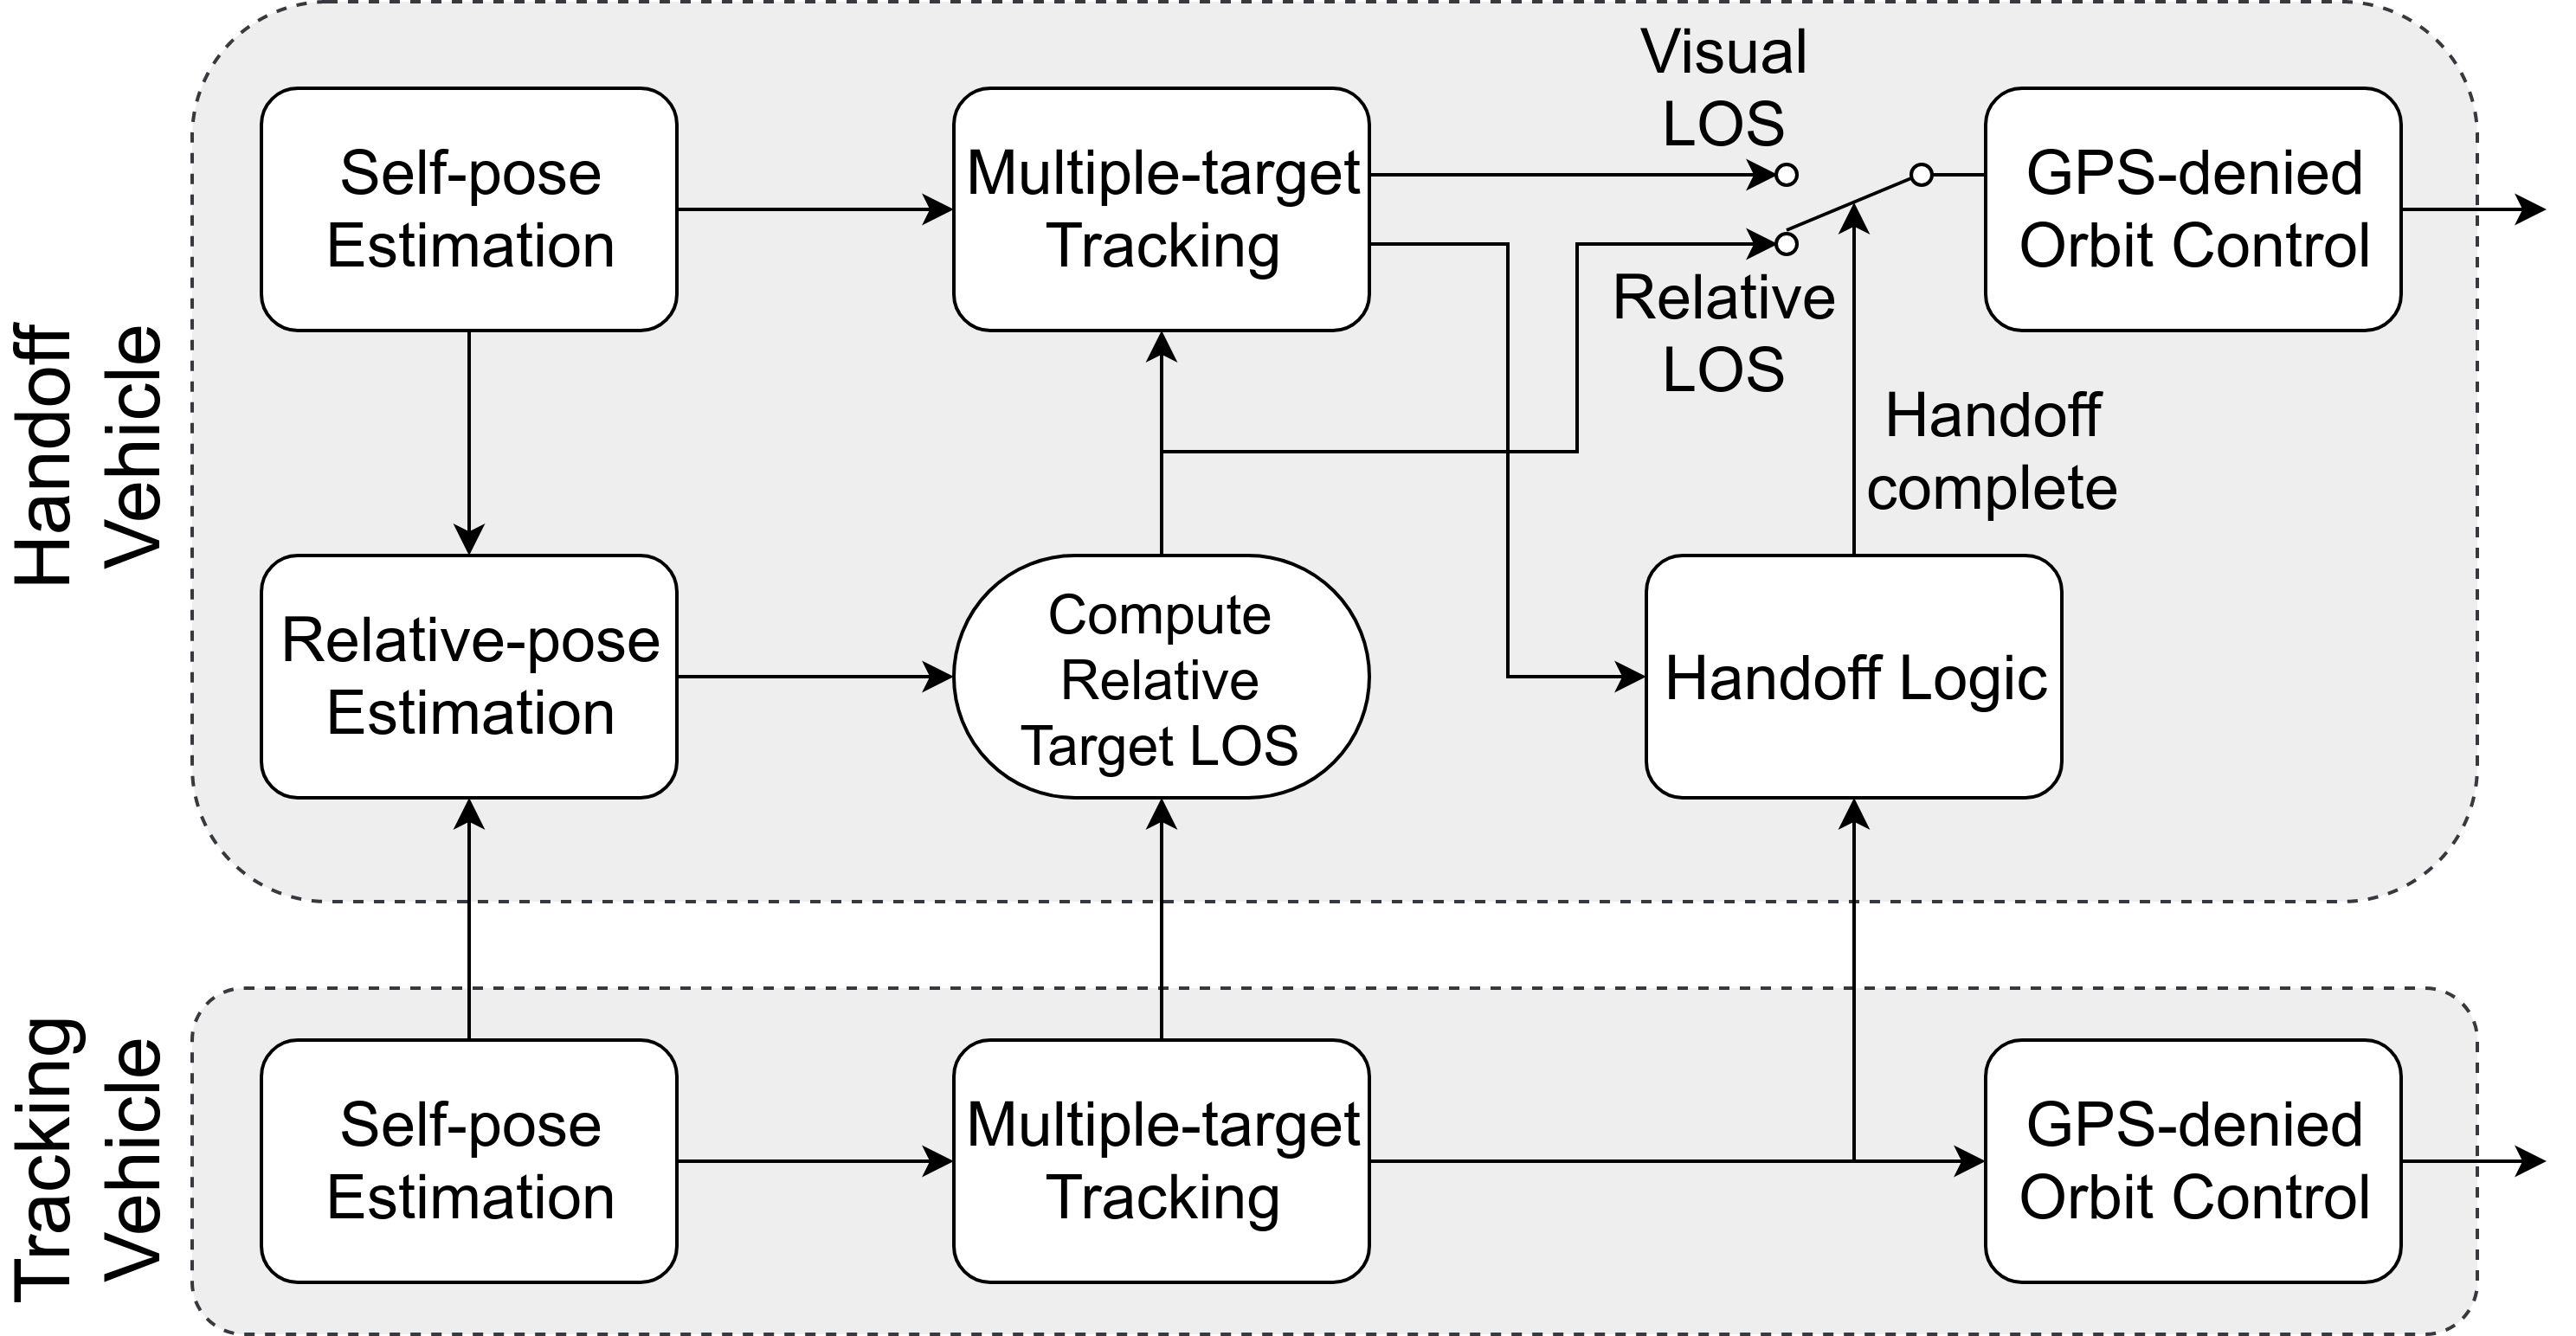
\includegraphics[width=1.0\textwidth]{figures/intro/handoff_block}
    \caption{Block diagram of the system components and information flow.}
    \label{fig:handoff_block}
\end{figure*}


This work addresses each of these challenges using either an extension of previous work or a novel solution to the problem. 
\begin{itemize}
  \item Self-pose estimation is addressed in Chapter~\ref{ch:self_pose}, and is solved using a complementary filter on $SO(3)$. and represents an extension of~\cite{Mahony11}.
  \item The estimates from the complimentary filter are inputs to a particle filter used to estimate the relative pose. A novel relative pose particle filter is derived in Chapter~\ref{ch:relative_pose}.
  \item The challenge of inserting a UAS into an orbit without GPS is solved using a controller that produces appropriate roll commands based on an estimated line of sight vector to the target. This controller is described in Chapter~\ref{ch:orbit_control}, and represents an extension of the orbit control algorithm described in~\cite{BeardMcLain12}.  
  \item The tracking and handoff UAS both utilize the Recursive-RANSAC (R-RANSAC) algorithm to visually track ground objects. While R-RANSAC was originally introduced in~\cite{NiedfeldtBeard14}, Chapter~\ref{ch:target_tracking} presents new results where the algorithm is used on a fixed-wing vehicle with a gimballed camera.
  \item Chapter~\ref{ch:handoff_logic} describes the algorithm used to perform the handoff logic, completing the moving target handoff problem.
  \item Chapter~\ref{ch:results} gives simulation results followed by some concluding remarks in Chapter~\ref{ch:conclusion}.
\end{itemize}

% !TEX root=../master.tex
\chapter{GPS-Denied Self-Pose Estimation}
\label{ch:self_pose}

A fundamental component of performing a target handoff without GPS is accurate estimation of the self-pose of each vehicle.
Without GPS, there is no global frame of reference that is common between the two vehicles. 
Accordingly, all information shared about the target must be coordinated using relative transformations. 
These relative transformations depend heavily upon each vehicle's estimate of its self-pose as well. 
Small errors in self-pose estimates are amplified by long distances and can lead to large errors in the estimated relative transformation between the two vehicles. 
This chapter will discuss methods for estimating the self-pose, followed by a discussion of estimating the relative-pose in Chapter~\ref{ch:relative_pose}. 
Both chapters are focused on estimation for fixed wing UAV in GPS-denied environments.

\section{Background}
There has been extensive work done on estimating the attitude of a fixed-wing aircraft both using non-linear~\cite{Mahony11} and linear~\cite{LiuZhouFu08} methods.
For this work we estimate the attitude state of the filter using a complimentary filter on SO(3), based upon the work done in \cite{Mahony11}. 
While the filter approach and algorithm remain the same, we do make a slight extension to the filter presented by Mahony et al. to better account for variability in the magnitude of the airspeed. The details of the filter, as well as our extension, will be discussed below.


% Two of these methods are discussed and compared here in an effort to identify which method provides the most accurate results for GPS-free fixed-wing estimation. In addition to making comparisons between existing filters, some improvements are proposed which extend previous work. First, a multiplicative extended Kalman filter (MEKF) for fixed-wing attitude estimation will be discussed, followed by an explanation of a non-linear complimentary filter which extend the work done in \cite{Mahony11}.
% % \section{Multiplicative Extended Kalman Filter}
%
% \subsection{Introduction}
% A common method of estimating fixed-wing attitude is by using an extended Kalman filter (EKF) to estimate the roll, pitch, and yaw of the aircraft. The main deficiencies of this approach are that (1) Euler angles contain a singularity when pitch is $\pm 90^{\degree}$ and (2) the repeated use of trigonometric functions can be computationally expensive.
% The multiplicative extended Kalman filter (MEKF) uses a quaternion, rather than Euler angles, to propagate the attitude state, eliminating the singularity and allowing for computationally efficient update and propagation steps. In order to propagate the attitude on $SO(3)$ the quaternion multiply operator must be used, hence the name "multiplicative extended Kalman filter." Because the quaternion is an over-parameterized representation of roll, pitch, and yaw, we cannot define a meaningful covariance for each of the four elements in the quaternion. Instead, we define the error covariance about the minimal representation, or error state, and perform the update using this error state. The covariance matrix, $\P$, is defined about the error state, which is one less in dimensionality than the full state vector. We must also derive error state versions of the propagation and measurement Jacobians in order to appropriately use the error state to update the estimates.
%
% Architecturally, the MEKF is very similar to the EKF. The primary difference is that because the covariance matrix is defined with respect to the error state, the update step outputs $\dx$, the error state, rather than producing $\x[\hat]$, as in the case of the EKF. Figures \ref{fig:ekf_diagram} and \ref{fig:mekf_diagram} show the respective high-level architectures of the EKF and the MEKF.
% \begin{figure}
% 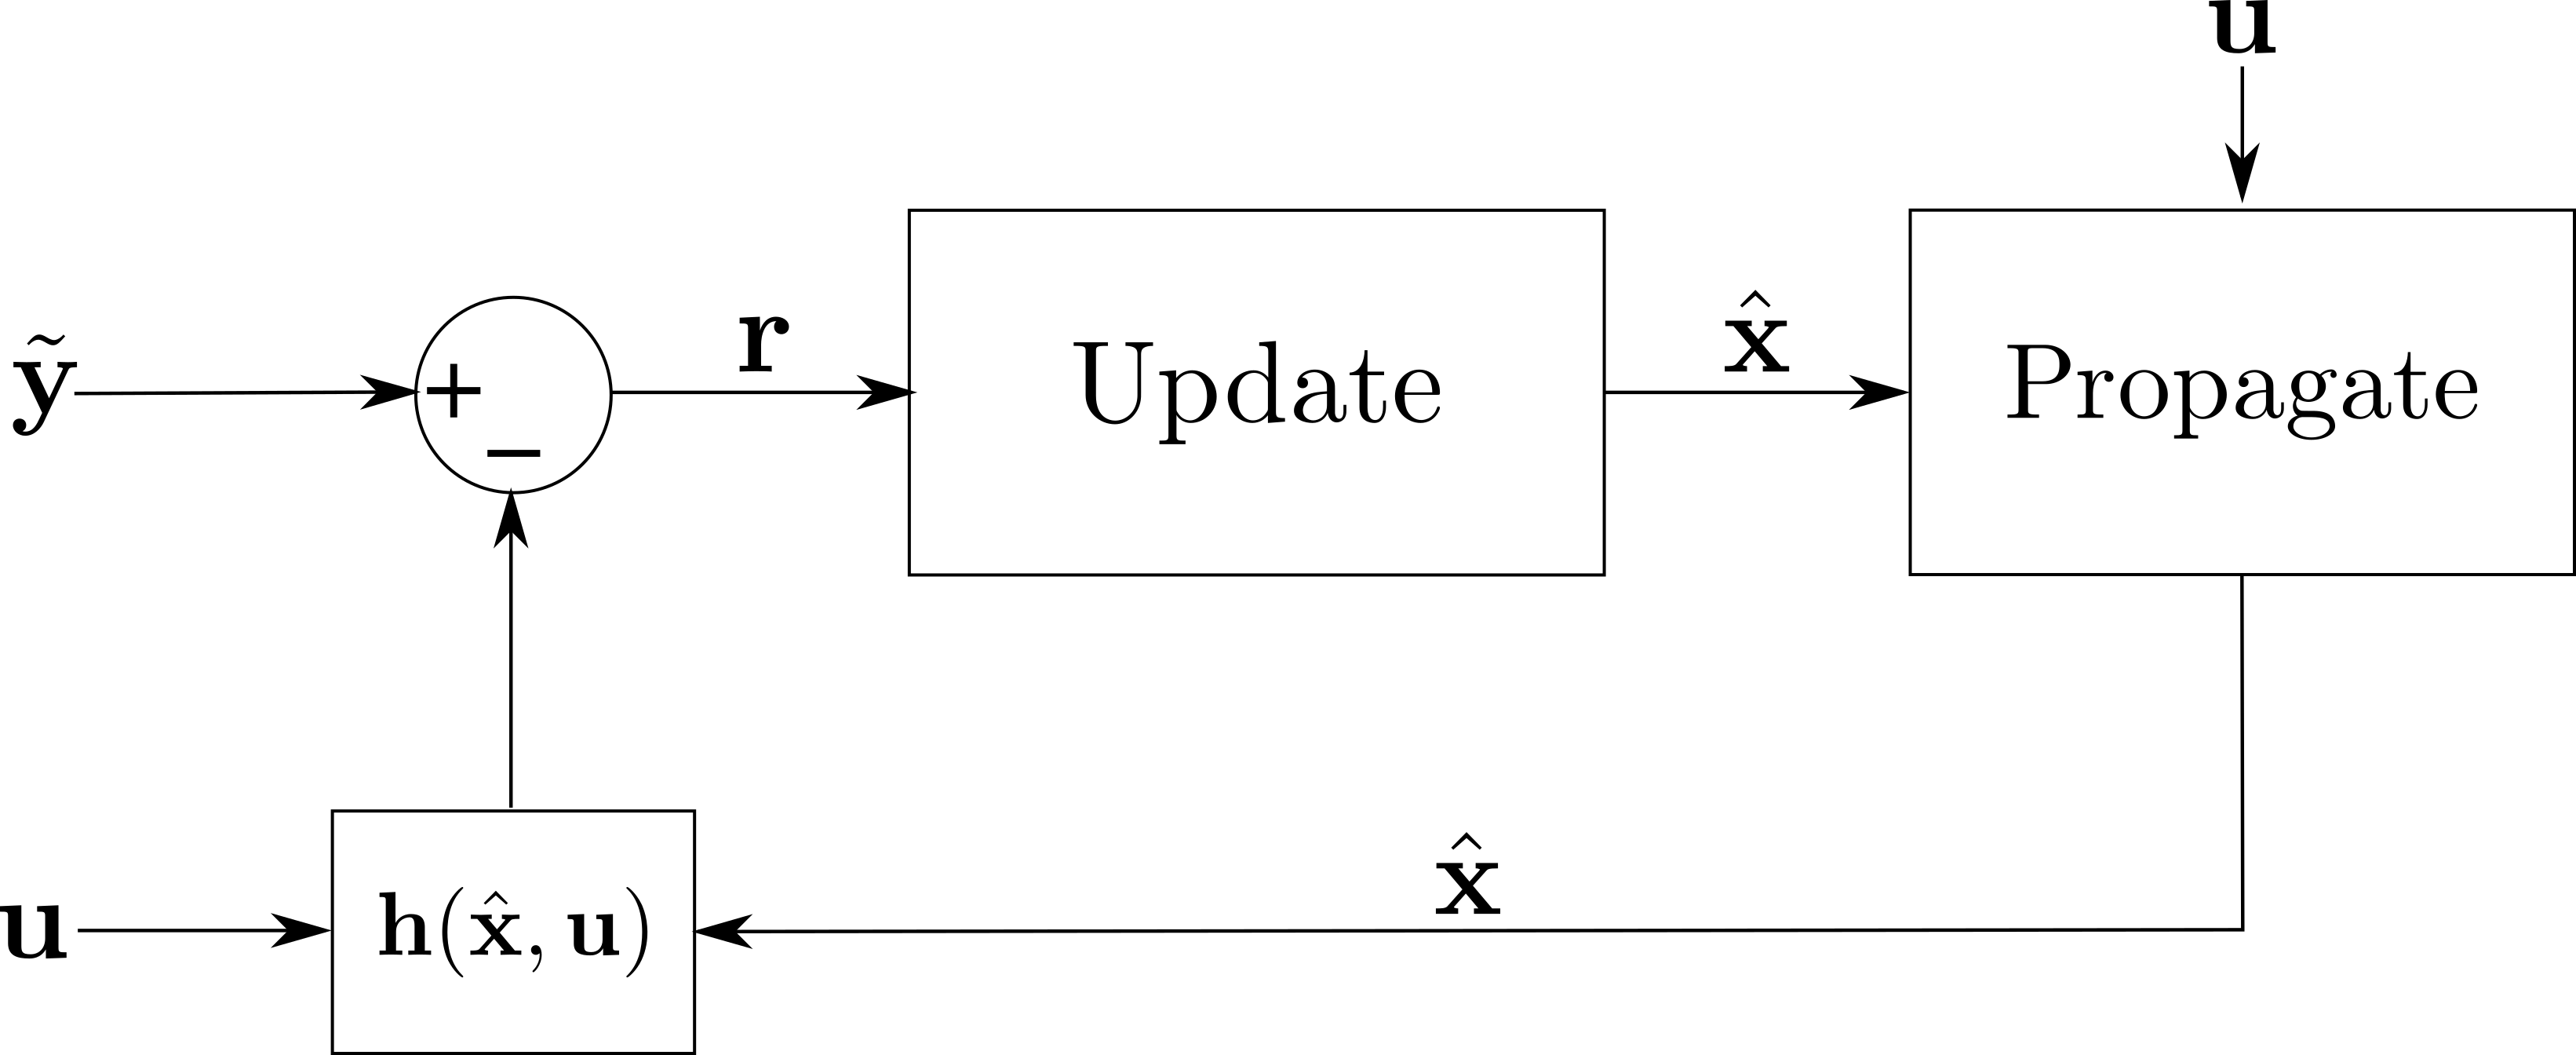
\includegraphics[width=\columnwidth]{figures/ekf_diagram.png}
% \caption{EKF flow diagram}
% \label{fig:ekf_diagram}
% \end{figure}
%
% \begin{figure}
% 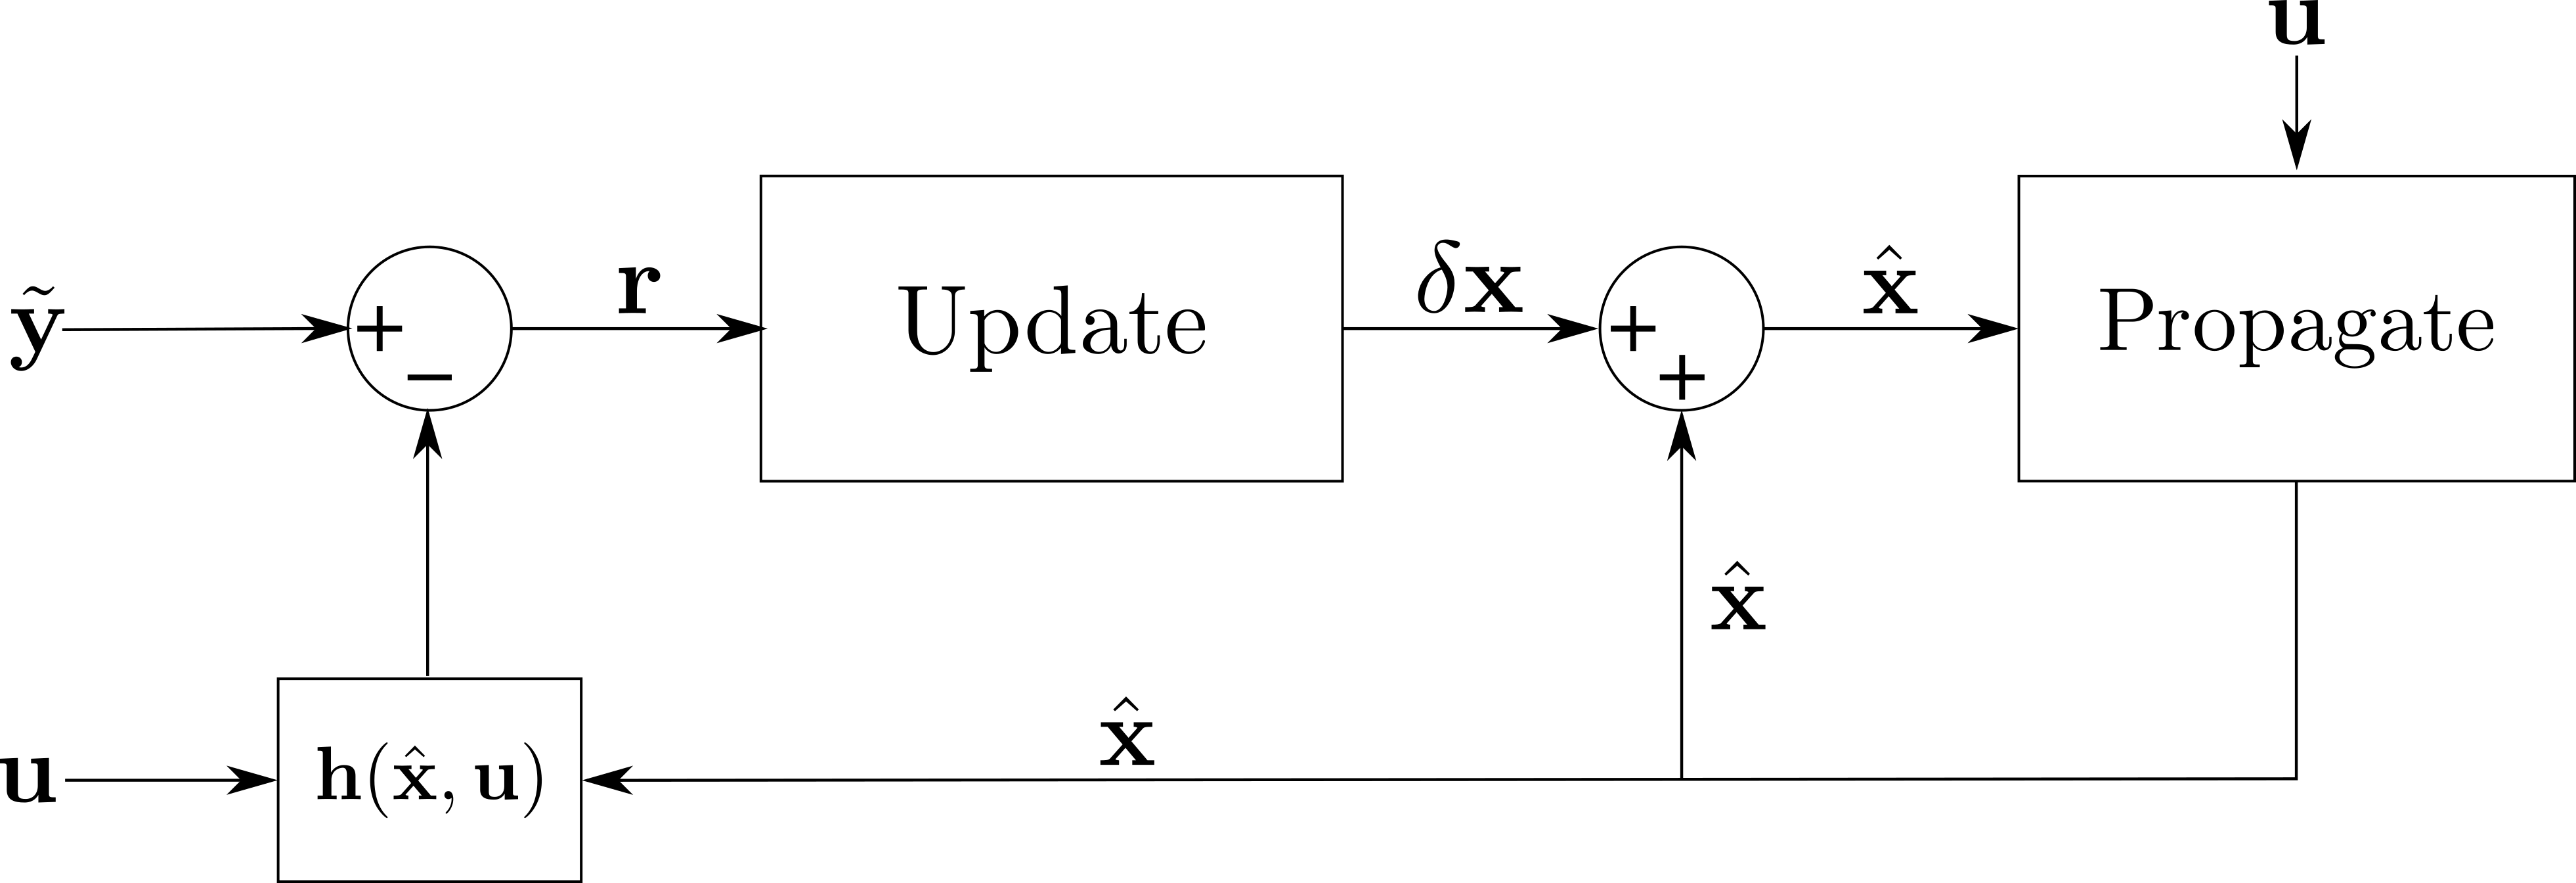
\includegraphics[width=\columnwidth]{figures/mekf_diagram.png}
% \caption{MEKF flow diagram}
% \label{fig:mekf_diagram}
% \end{figure}
%
% The MEKF presented here draws heavily from \cite{RMEKF}, but also offers some unique contributions. This implementation focuses specifically on fixed-wing aircraft and makes some improvements based on the dynamics specific to fixed-wing vehicles. For example, the filter concurrently estimates the airspeed vector using an estimate of the angle of attack along with estimating gyro biases to improve the attitude estimates. The filter also estimates the attitude independent of GPS data.
%
%
% \subsection{Quaternions}
% Before describing the core implementation of the filter, it is important to have a basic understanding of quaternions and their properties.
% This section provides an overview of the quaternion operations and conventions used in this implementation. This section is intended to be used as a useful reference, especially for the implementation of the filter. It is not, however, a comprehensive guide to quaternions and does not provide the full derivation for most of the equations used. For a more in-depth resource on quaternions, we refer the reader to \cite{eq:MEKF},~\cite{Trawny05}.
% \label{sec:quaternions}
%
%
% \subsubsection{Definitions}
%
% Quaternions are a hyper-complex four-dimensional representation of attitudes and rotations. We can define a quaternion, generally as
% % %%
% % \comment{REVIEW: Does this need to be vector or scalar notation}
% % %%
% \begin{equation}
% \q = \qw + q_x \ii + q_y \jj + q_z \kk \;
% \end{equation}
% where $\q \in \mathbb{H}$.

% Quaternions can be represented in multiple ways, each resulting in slightly different version of the basic definitions and operations used. This section will describe the conventions used for all quaternion variables and operations throughout the paper.

% Specifically, we will be using the Hamiltonian definition of a quaternion, as opposed to JPL notation (\cite{JPL}). The Hamiltonian definition of a quaternion is given by
% \begin{align} \label{eq:complex_products}
% \begin{split}
% \ii \jj = -\jj \ii &= \kk \;, \\
% \jj \kk = -\kk \jj &= \ii \;, \\
% \kk \ii = -\ii \kk &= \jj \;, \\
% \ii^2 = \jj^2 = \kk^2 = \ii \jj \kk &= -1 \;.
% \end{split}
% \end{align}

% For convenience, we will define the quaternions as
% \begin{equation}
%   \label{eq:q_definition}
%   \q = \begin{bmatrix} \qvec \\ \qw \end{bmatrix} \;,
% \end{equation}
% where $\qvec$ is the vector component, representing the axis of rotation, and $\qw$ is the scalar component, representing the magnitude of rotation. The vector portion, $\qvec$, is defined as
% \begin{equation}
%   \label{eq:qvec}
% 	\qvec=\begin{bmatrix} q_x & q_y & q_z \end{bmatrix}^\transpose \;.
% \end{equation}


% \subsubsection{Quaternion multiplication}

% Quaternions have no defined addition or subtraction operators. Instead the quaternion multiplication operator is used to combine quaternions. The Hamiltonian quaternion multiply is defined according to
% \begin{align} \label{eq:q_mult}
% \p \otimes \q &=
%     \begin{bmatrix}
%     \pw \I + \skewmat{\pvec} & \pvec \\
%     -\pvec^\transpose & \pw
%     \end{bmatrix}
%     \begin{bmatrix} \qvec \\ \qw \end{bmatrix}\; \\
% &= \begin{bmatrix}
%     \qw \I - \skewmat{\qvec} & \qvec \\
%     -\qvec^\transpose & \qw \end{bmatrix}
%     \begin{bmatrix} \pvec \\ \pw \end{bmatrix}\;.
% \end{align}
% Also note that $\skewmat{\cdot}$ defines the skew-symmetric operator, such that
% \begin{equation} \label{eq:skewmat_def}
% \skewmat{\vect{a}} \triangleq \begin{bmatrix}
% 0 & -a_z & a_y \\
% a_z & 0 & -a_x \\
% -a_y & a_x & 0 \end{bmatrix}.
% \end{equation}


% \subsubsection{Error state}

% We can define the true attitude quaternion state as
% \begin{equation} \label{eq:q_actual}
% \q = \q[\hat] \otimes \dq
% \end{equation}
% where $\q[\hat]$ is the estimated attitude and $\dq$ is the error in the attitude.
% Solving for $\dq$ in \eqref{eq:q_actual}, we get
% \begin{equation}
% \dq = \q[\hat]^{-1} \otimes \q \;.
% \end{equation}
% As previously mentioned, we cannot define a covariance about a quaternion, so we use a minimal representation of the quaternion error, denoted by $\dth$ such that
% \begin{equation} \label{eq:dq}
% \dq = \exp\left(\half \dth\right) \;
% \end{equation}
% where $\exp(\cdot)$ is defined by \eqref{eq:quat_exp}.
% When $\dq[\bar]$ is small, we can use a first order approximation of \eqref{eq:dq},
% \begin{equation}
% \dq = \begin{bmatrix} \half \dth \\ 1 \end{bmatrix},
% \end{equation}
% which leads to
% \begin{equation}
% \dth = 2\dq[\bar] \;.
% \end{equation}

% \subsubsection{Exponential mapping}

% In order to map the error state vector, $\dth$, which is a minimal representation in $\mathbb{R}^3$, to the quaternion in $SO(3)$, we use an exponential mapping, defined as
% \begin{equation} \label{eq:quat_exp}
%   \exp(\delta) \triangleq \begin{bmatrix} \sin\norm{\delta}\frac{\delta}{\norm{\delta}} \\ \cos\norm{\delta} \end{bmatrix}\;.
% \end{equation}
% It is important to note that as $\norm{\delta} \approaches 0$, the exponential mapping becomes numerically unstable. Therefore, when $\norm{\delta}$ is sufficiently small, we can approximate the exponential mapping by using its limit, given by
% \begin{equation} \label{eq:exp_lim}
% \lim_{\norm{\delta}\approaches 0}\exp(\delta) = \begin{bmatrix} \delta \\ 1 \end{bmatrix}\;.
% \end{equation}

% The exponential mapping, in combination with the $\otimes$ operator, allows us to update the quaternion by some minimal representation error state, $\dth$, while still remaining completely on the $SO(3)$ manifold. This is performed according to
% \begin{equation} \label{eq:q_update}
% \q^+ = \q^- \otimes \exp\left(\half\dth\right) \;.
% \end{equation}
% Or, when $\norm{\dth}$ is small, we use the limit of the exponential, given in \eqref{eq:exp_lim}, resulting in
% \begin{equation}
% \q^+ = \q^- \otimes \begin{bmatrix} \half\dth \\ 1 \end{bmatrix} \;.
% \end{equation}
% % Commonly, linear approximations of this mapping are used and then normalized back to the manifold, but using this exponential mapping allows us to remain on the manifold and minimize linearization errors.

% In some recent literature (\cite{boxplus_herztberg}), the combination of using quaternion multiplication and the exponential mapping in order to update a quaternion is also referred to as the ''boxplus'' operator ($\boxplus$). For example, equation \eqref{eq:q_update} could be written as
% \begin{equation}
% \q^+ = \q^- \boxplus \dth
% \end{equation}
% using boxplus notation.
% While the two operations are synonymous, we will use the notation in equation \eqref{eq:q_update} for verbosity.


% \subsubsection{Rotations}

% It is also often necessary to produce a rotation matrix from the quaternion attitude state. In this paper, quaternion rotation matrices are computed according to
% \begin{equation} \label{eq:Rq}
%   \R(\q) = \qw^2 \I - 2\qw \skewmat{\qvec} + \qvec\qvec^\transpose + \skewmat{\qvec}^2 \;.
% \end{equation}
% It is also possible to represent $\skewmat{\qvec}^2$ as
% \begin{equation}
% \skewmat{\qvec}^2 = \qvec \qvec^\transpose - (1 - \qw^2)\I \;
% \end{equation}
% and rewrite \eqref{eq:Rq} as
% \begin{equation}
% \R(\q) = (2\qw^2 - 1)\I - 2\qw\skewmat{\qvec} + 2\qvec\qvec^\transpose \;.
% \end{equation}


% \subsubsection{Time derivative}

% In this implementation of the MEKF, the first order quaternion derivative is used, given by
% \begin{equation} \label{eq:qhatdot}
%   \q[\hatdot] = \half \q[\hat] \otimes \begin{bmatrix} \angvel[\hat] \\ 0 \end{bmatrix} \;.
% \end{equation}
% This can also be expressed as
% \begin{equation}
% \q[\hatdot] = \half \Omega(\angvel[\hat]) \q[\hat]
% \end{equation}
% where
% \begin{equation} \label{eq:Omega}
%   \bOmega(\angvel) = \begin{bmatrix} 0 & \omega_z & -\omega_y & \omega_x \\
%                                       -\omega_z & 0 & \omega_x & \omega_y \\
%                                       \omega_y & -\omega_x & 0 & \omega_z \\
%                                       -\omega_x & -\omega_y & -\omega_z & 0 \end{bmatrix} \;.
% \end{equation}


% \subsubsection{Time integration}

% Quaternion integration is primarily based upon trying to perform some incremental update,
% \begin{equation}
% \q_{t + \Delta t} = \q_t \otimes \q_{\Delta t}.
% \end{equation}
% Zero-th order integration assumes a constant nominal angular velocity, $\angvel_0$, and is given by
% \begin{equation}
% \q_{t + \Delta t} = \q_t + \Delta t \left(\half \q_t \otimes \begin{bmatrix} \angvel_0 \\ 0 \end{bmatrix} \right) \;.
% \end{equation}
% Note that this form of quaternion integration will depart slightly from the $SO(3)$ manifold, so the quaternion must be manually normalized back onto the manifold.
% A first order quaternion integrator is used to propagate the quaternion estimate, which assumes that angular velocity is evolving linearly between integration steps.
% The integration, as derived in \cite{Trawny05}, is given by
% \begin{equation} \label{eq:q_int}
% % \small
%   \q(t_{k+1}) = \Bigg[ \matexp\left(\half \bOmega(\bar{\angvel})\Delta t \right) + \frac{1}{48} \bigg( \bOmega\big( \angvel( t_{k+1})\big) \bOmega\big( \angvel(t_k)\big) - \bOmega\big( \angvel( t_{k})\big) \bOmega\big( \angvel(t_{k+1})\big)\bigg) \Delta t^2 \Bigg] \q(t_k)
% \end{equation}
% where $\matexp\left(A\right)$ is the matrix exponential,
% $\Omega(\angvel)$ is given by \eqref{eq:Omega}, and
% \begin{equation}
%   \bar{\angvel} = \frac{\angvel(t_{k+1}) + \angvel(t_k)}{2} \;.
% \end{equation}

% % \subsection{Euler angle/quaternion relationship}
% \subsubsection{Euler angle decomposition}

% It is often useful to be able to convert between Euler angle and quaternion representations of the attitude.
% % Quaternion to euler
% For a given quaternion,
% $$ \q = \begin{bmatrix} q_x \\ q_y \\ q_z \\ \qw \end{bmatrix} \;, $$
% the corresponding roll ($\phi$), pitch ($\theta$), and yaw ($\psi$) are given by
% \begin{align}
% \phi &= \text{atan}\left(\frac{2 \qw q_x + 2 q_y q_z}{q_z^2 - q_x^2 - q_y^2 + \qw^2}\right) \;, \\
% \theta &= \text{asin}\left(2 \qw q_y - 2 q_x q_z\right) \;, \\
% \psi &= \text{atan}\left(\frac{2 \qw q_z + 2 q_x q_y}{q_x^2 - q_y^2 - q_z^2 + \qw^2}\right) \;. \label{eq:quat_psi}
% \end{align}
% % Euler to Quaternion
% Conversely, for a given set of Euler angles, the corresponding quaternion can be constructed according to
% \begin{align}
% q_x &= \cos\frac{\psi}{2} \cos\frac{\theta}{2} \sin\frac{\phi}{2} - \sin\frac{\psi}{2} \sin\frac{\theta}{2} \cos\frac{\phi}{2} \;, \\
% q_y &= \cos\frac{\psi}{2} \sin\frac{\theta}{2} \cos\frac{\phi}{2} + \sin\frac{\psi}{2} \cos\frac{\theta}{2} \sin\frac{\phi}{2} \;, \\
% q_z &= \sin\frac{\psi}{2} \cos\frac{\theta}{2} \cos\frac{\phi}{2} - \cos\frac{\psi}{2} \sin\frac{\theta}{2} \sin\frac{\phi}{2} \;, \\
% \qw &= \cos\frac{\psi}{2} \cos\frac{\theta}{2} \cos\frac{\phi}{2} + \sin\frac{\psi}{2} \sin\frac{\theta}{2} \sin\frac{\phi}{2} \;.
% \end{align}


% %%%%%%%%%%%%%%%%%%%%%%%%%%%%%%%%%%%%%%%%%%%%%%%%%%%%%%%%%%%%%%%%%%%%%%%
% %%%%%%%%%%%%%%%%%%%%%%%% FILTER IMPLEMENTATION %%%%%%%%%%%%%%%%%%%%%%%%
% %%%%%%%%%%%%%%%%%%%%%%%%%%%%%%%%%%%%%%%%%%%%%%%%%%%%%%%%%%%%%%%%%%%%%%%
% \vspace{2em}
% \subsection{Filter Implementation}
% \label{sec:implemenation}
% Many of the equations used here are based upon the MEKF framework given in~\cite{RMEKF}. This section will seek to show derivations for novel changes to the basic MEKF implementation and other additions which are specific to a fixed-wing model, but we refer the reader to other MEKF literature for in depth derivations of the basic filter framework (\stcomment{cite key MEKF papers here}).\\

% %%%%%%%%%%%%%%%%%%%%%%%%%%%%% DEFINITIONS %%%%%%%%%%%%%%%%%%%%%%%%%%%%%
% \subsubsection{Definitions}

% The MEKF implemented here primarily seeks to accurately estimate the attitude quaternion, but the state also includes gyro bias and angle of attack to help improve the estimator's accuracy.
% The state is defined as
% \begin{equation}
%     \x = \begin{bmatrix} \q \\ \gbias \\ \alpha \end{bmatrix}
% \end{equation}
% where $\q$ is the attitude quaternion, $\gbias$ represents the gyro biases along the x, y, and z axes, and $\alpha$ is the vehicle's angle of attack.

% % [ST] TODO: with the airspeed in the input, do we need to add airspeed noise throughout and adjust our jacobians?
% The input vector is composed of the gyro and airspeed sensor measurements and is given by
% $$ \u = \begin{bmatrix} \tilde{\angvel} \\ v_a \end{bmatrix}, $$
% where
% $$ \tilde{\angvel} = \begin{bmatrix} \tilde{\omega}_x \\ \tilde{\omega}_y \\ \tilde{\omega}_z \end{bmatrix}.  $$
% and $v_a$ is the airspeed.
% We define our measurement as the accelerometer sensor data, $\accel[\tilde]$, and the heading measurement extracted from the magnetometer, $\tilde{\psi}$, according to
% $$ \y = \begin{bmatrix} \tilde{\accel} \\ \tilde{\psi} \end{bmatrix} =
%         \begin{bmatrix} \tilde{a}_x & \tilde{a}_y & \tilde{a}_z & \tilde{\psi} \end{bmatrix}^{\transpose} \;.$$

% The heading information can be determined from the magnetometer data, $\magnet$, by
% rotating the sensor data into the vehicle 1 (unpitched, unrolled) frame, isolating the heading angle, and factoring in the magnetic field declination, $\magdec$, according to
% \begin{subequations} \label{eq:mag2heading}
% \begin{align}
%   \magnet^{v1} &= \Rot{b}{v1}\magnet \\
%   % [ST] TODO: check for other atan2 implementations
%   \psimag &= \atantwo(\magnet^{v1}_{y}, \magnet^{v1}_{x}) \\
%    \tilde{\psi} &= \magdec - \psimag \;.
% \end{align}
% \end{subequations}
% The value of $\magdec$ can be predetermined based upon the approximate latitude and longitude at which the aircraft will be flown.
% Figure~\ref{fig:magnetometer} gives a geometrical representation of the magnetometer-based heading measurement.
% \begin{figure}[hbt]
%   \centering
%   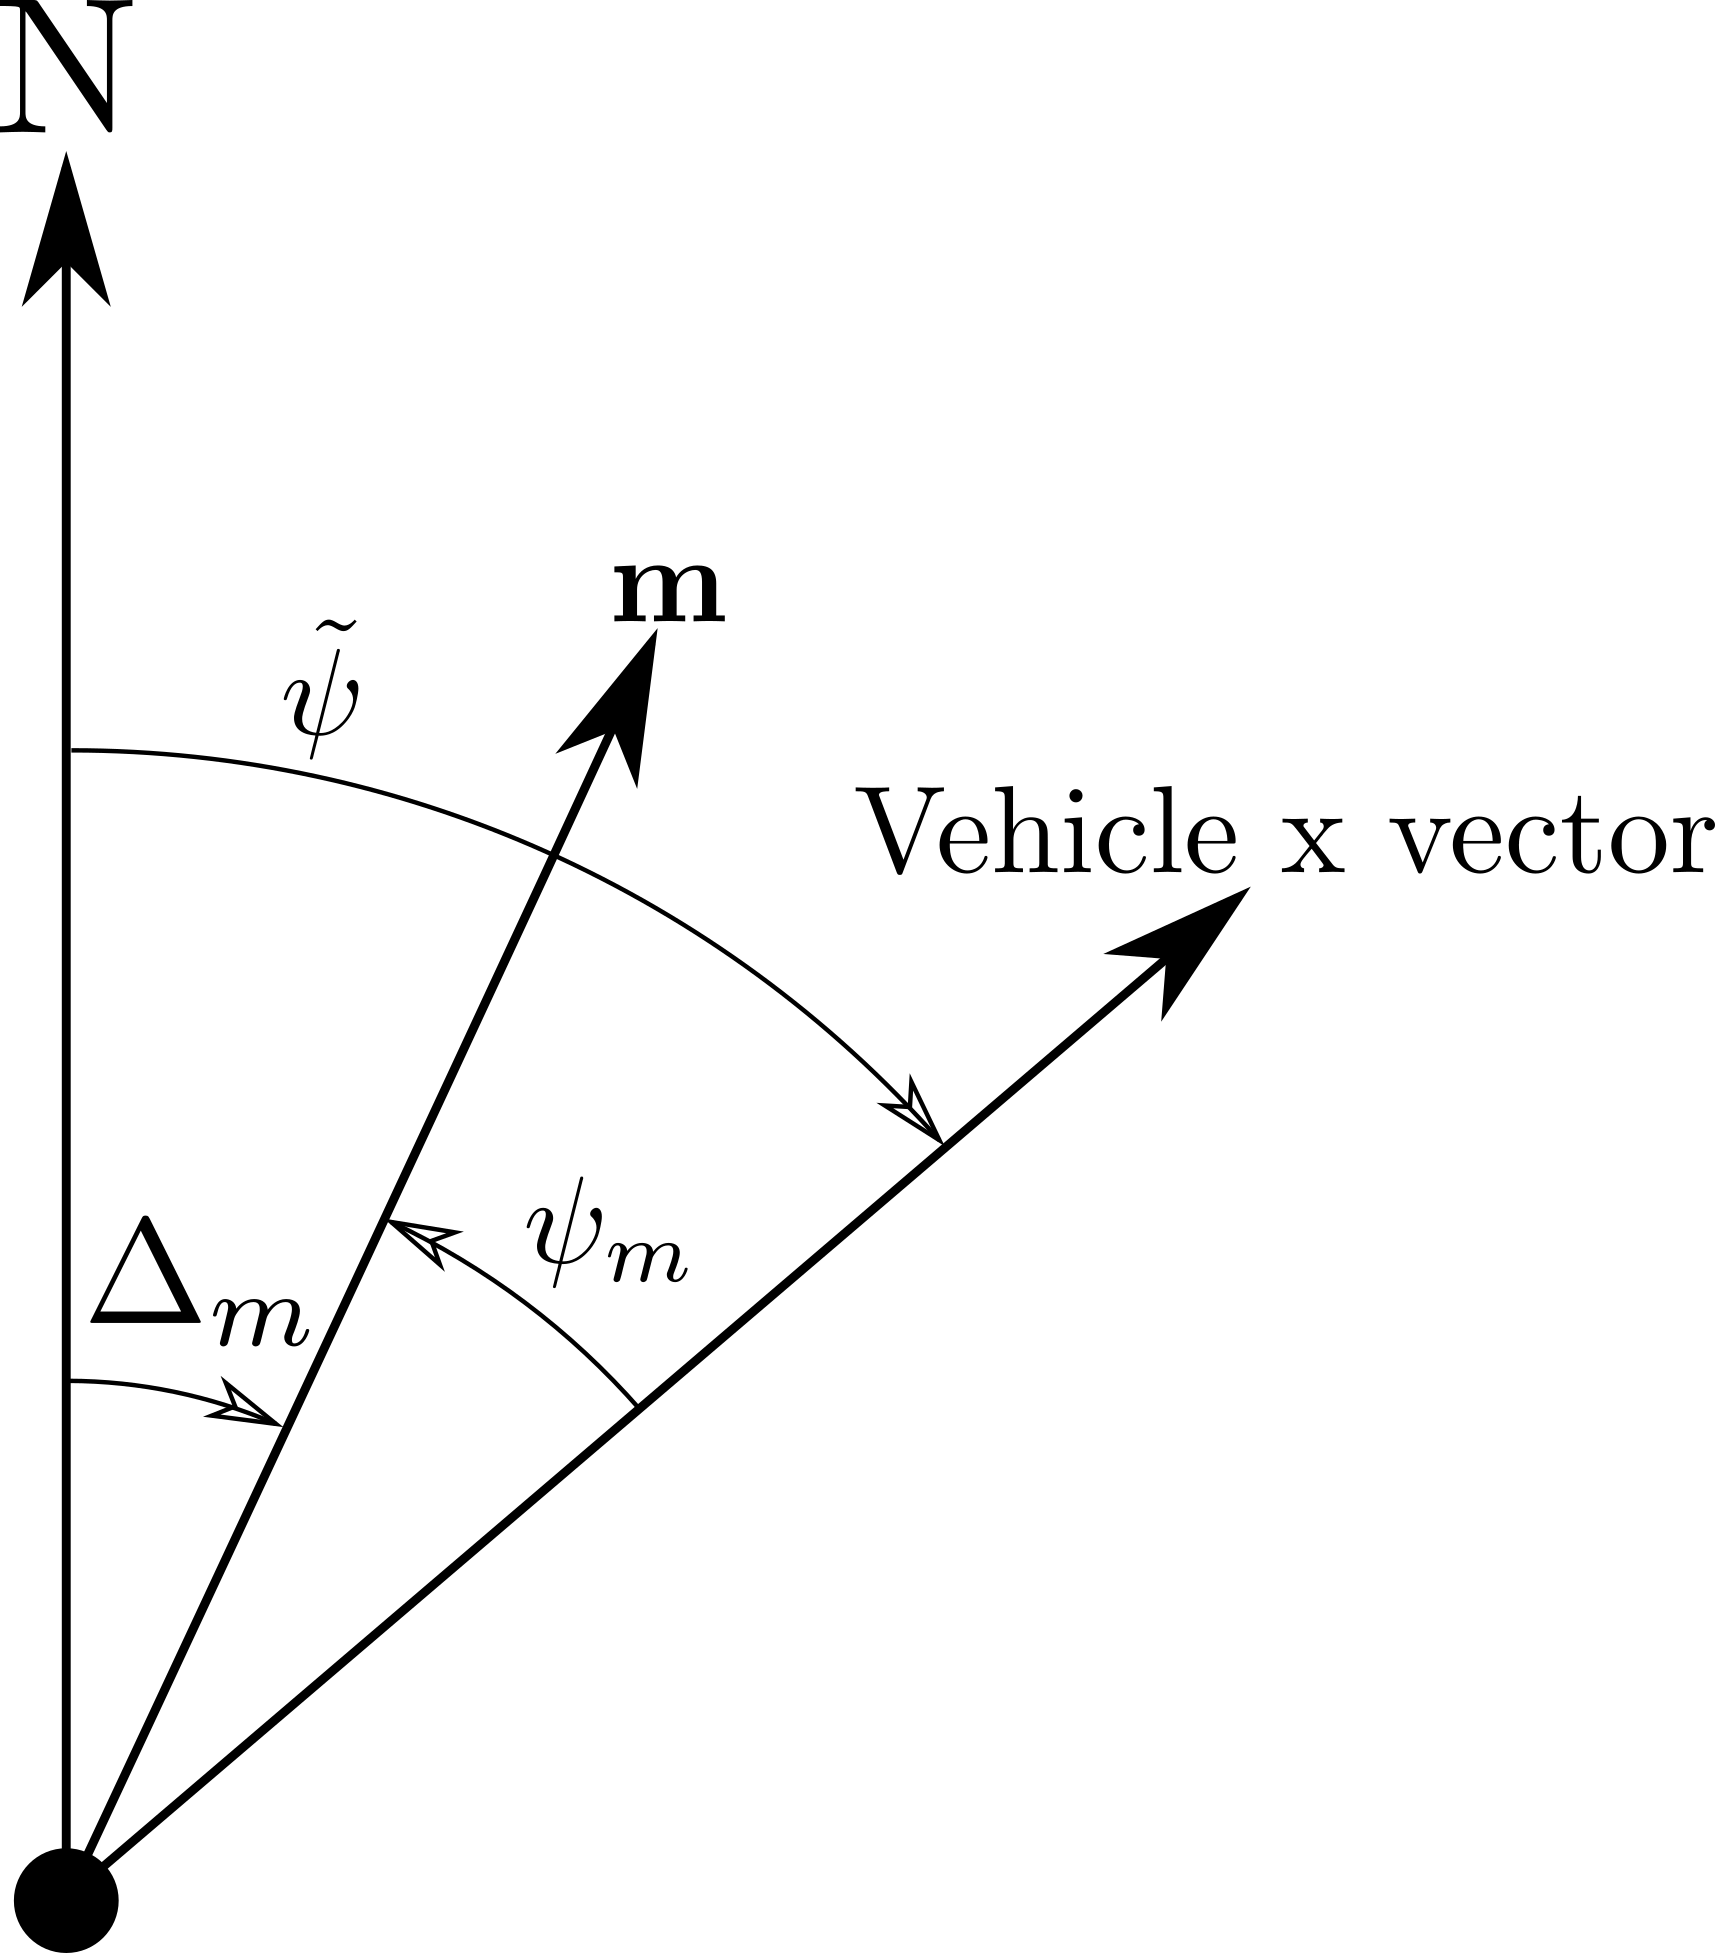
\includegraphics{figures/mekf_mag_geom}
%   \caption{XY-plane representation of heading measurement from magnetometer sensor reading.}
%   \label{fig:magnetometer}
% \end{figure}
% \newline

% %%%%%%%%%%%%%%%%%%%%%%%%%%%%% PROPAGATION %%%%%%%%%%%%%%%%%%%%%%%%%%%%%
% \subsubsection{State propagation}
% The state propagation dynamics are denoted by
% \begin{equation} \label{eq:estimator_dynamics}
%  \x[\hatdot] = \f(\x[\hat], \u) \;.
% \end{equation}
% However, because the not all of the dynamics are linear, the propagation step is best expressed in terms of the individual state components.

% The dynamics of a quaternion are often defined according to the first order time derivative in \eqref{eq:qhatdot} as
% \begin{equation*}
% \q[\hatdot] = \half \q[\hat] \otimes \begin{bmatrix} \angvel[\hat] \\ 0 \end{bmatrix} \;.
% \end{equation*}
% However, in practice, we will use the first order quaternion integrator given in \eqref{eq:q_int}.

% We assume the gyro bias is relatively constant, with some noise and slow, unpredictable drift, so we define the bias dynamics according to
% \begin{equation} \label{eq:gbias_dynamics}
%   \gbias[\hatdot] = \vect{0} \;.
% \end{equation}

% The estimated angle of attack is propagated according to a linearized dynamic model, adapted from the model used in \cite{Mahony11}, given by
% \begin{equation}
%   \hatdot{\alpha} = -\frac{c_0(v_a)}{v_a}\hat{\alpha} + \dot{\theta} + (\alpha_0(v_a))
% \end{equation}
% where
% \begin{equation} \label{eq:c0_Va}
% c_0(v_a) = \frac{k_\delta - k_T v_a^2}{m}
% \end{equation}
% and
% \begin{equation}
% \alpha_0(v_a) = \frac{g}{v_a} - \frac{k_L}{m}v_a \;.
% \end{equation}
% The function $c_0(v_a)$ represents the effects of the thrust force and $\alpha_0(v_a)$ acts as a set point needed to maintain level flight, based on airspeed and the lift force.
% In \cite{Mahony11}, $c_0$ and $\alpha_0$ are constants, but we have replaced them with simple functions of airspeed in order to maintain greater model accuracy across varying speeds. The derivation for this adaptation is given in Appendix \ref{append:alpha_derivation}.

% For our implementation we achieved fairly good estimation of $\alpha$ using the following values for our constants:
% %%
% % \todo[inline]{Update or remove these constants}
% %%
% \begin{align*}
%   k_\delta &= 40 \\
%   k_T &= -4.07 \\
%   k_L &= 0.245 \\
%   m &= 3.92\text{ kg} \;.
% \end{align*}
% These values are system dependent and can be obtained experimentally.

% Because the covariance matrix represents the spread of the error state, in order to compute the propagation Jacobians, we need to derive an error state measurement model, $\bar{\f}$, given by
% \begin{subequations} \label{eq:dxdot_error}
% \begin{align}
% \dx[\dot] &= \f[\bar](\dx,\noiseu,\x[\hat],\u) + \noise \;. \\
% 		&= \f(\x, \u + \noiseu) - \f(\x[\hat], \u) \\
%         &= \f(\x[\hat] + \dx, \u + \noiseu) - \f(\x[\hat], \u) \;.
% \end{align}
% \end{subequations}
% %%
% % \todo[inline]{Add derivations here}
% %%
% The first-order approximation of the error-state dynamics are
% %\begin{subequations}
% \begin{align}
%   \label{eq:error_dynamics_dth}
%   \dth[\dot] &\approx -\skewmat{\angvel[\tilde] - \gbias[\hat]}\dth - \dgbias - \noiseu_{\angvel} \\
%   \label{eq:error_dynamics_dgbias}
%   \dgbias[\dot] &= \noise_{\gbias} \\
%   \label{eq:error_dynamics_dalpha}
%   \dot{\dalpha} &= \frac{-(k_\delta - k_T v_a^2)}{mv_a}\dalpha - (\dgbias + \noiseu_{\angvel})\cdot\vect{e}_2 \;,
% \end{align}
% where $\vect{e}_2$ represents world frame $y$-vector, $\begin{bmatrix} 0 & 1 & 0 \end{bmatrix}^\transpose$. We refer the reader to \cite{RMEKF} for a derivation of \eqref{eq:error_dynamics_dth}, but derivations of \eqref{eq:error_dynamics_dgbias} and \eqref{eq:error_dynamics_dalpha} are given in Appendix \ref{append:error_dyn_derivation}.

% From $\bar{\f}$ we can derive the error state propagation Jacobians such that
% \begin{align}
%  \F &= \pard{\f[\bar](\dx,\noiseu,\x[\hat],\u)}{\dx} \;,
%  \label{eq:F}
% \end{align}
% \begin{align}
%  \G &= \pard{\f[\bar](\dx,\noiseu,\x[\hat],\u)}{\noiseu} \;,
%  \label{eq:G}
% \end{align}
% with $\noiseu$ being the input noise, and where $\Q_{\u}$ and $\Q_{\x}$ are the noise covariance matrices for the input and state, respectively.
% Defining $\angvel[\hat] = \angvel[\tilde] - \gbias[\hat]$, we can construct our Jacobians as
% \begin{equation}
%   \label{eq:F_mat}
%   \F = \begin{bmatrix} -\skewmat{\angvel[\hat]} & -\I_{3\By3} & \vect{0}_{3\By1} \\ \vect{0}_{3\By3} & \vect{0}_{3\By3} & \vect{0}_{3\By1} \\ \vect{0}_{1\By3} & -\vect{e}_2 & \frac{-(k_\delta - k_T v_a^2)}{mv_a} \end{bmatrix} \;,
% \end{equation}
% \begin{equation}
%   \label{eq:G_mat}
%   \G = \begin{bmatrix} -\I_{3\By3} & \vect{0}_{3\By1} \\ \vect{0}_{3\By3} & \vect{0}_{3\By1} \\ -\vect{e}_2 & 0 \end{bmatrix} \;.
% \end{equation}

% Finally, the error-state covariance, $\P$, is propagated according to
% \begin{equation} \label{eq:P_predict_step}
% \P[\dot] = \F \P + \P \F^\transpose + \G \Q_{\u} \G^\transpose + \Q_{\x} \;.
% \end{equation}

% %%%%%%%%%%%%%%%%%%%%%%%%%%%%%%%% UPDATE %%%%%%%%%%%%%%%%%%%%%%%%%%%%%%%%
% \subsection{Measurement update}
% The state estimates are updated each time a sensor measurement is received. We will first outline the measurement update step for a general measurement and then show the derivations specific to each sensor.
% \subsubsection{General update}
% Let $y$ represent some general sensor measurement where
% \begin{equation}
% y = \h(\x[\hat], \u) \;.
% \end{equation}
% Because the covariance matrix represents the spread of the error state, in order to compute the measurement Jacobians, we need to derive an error state measurement model, $\bar{\h}$, given by
% \begin{subequations}
% \begin{align}
% \bar{\h}(\dx, \noiseu, \x[\hat], \u)  &= \h(\x, \u + \noiseu) - \h(\x[\hat], \u) \\
%                                         &= \h(\x[\hat] + \dx, \u + \noiseu) - \h(\x[\hat], \u) \;.
% \end{align}
% \end{subequations}
% Then, using $\h[\bar]$, the measurement Jacobians can be defined as
% \begin{equation} \label{eq:H}
% \H = \pard{\h[\bar](\dx,\noiseu,\x[\hat],\u)}{\dx} \;,
% \end{equation}
% \begin{equation} \label{eq:J}
% \mat{J} = \pard{\h[\bar](\dx,\noiseu,\x[\hat],\u)}{\noiseu} \;.
% \end{equation}
% The residual, $\textbf{r}$, which represents the difference between the sensor measurement and the measurement model, is defined as
% \begin{equation} \label{eq:residual}
%   \textbf{r} = y - \h(\x[\hat], \u) \;,
% \end{equation}
% and the residual uncertainty is given by
% \begin{equation} \label{eq:S}
%   \mat{S} = \H\P\H^\transpose + \J\Q_{\u}\J^\transpose + \R \;.
% \end{equation}
% We can then define the Kalman gain as
% \begin{equation} \label{eq:kalman}
%   \K = \P\H^\transpose \mat{S}^{-1} \;.
% \end{equation}
% Using the Kalman gain, we can update our error state values. The propagation of $\dx$ is given by
% \begin{equation} \label{eq:dx_plus}
%   \dx^+ = \dx^- + \K\textbf{r} \;.
% \end{equation}
% Note, however, that $\dx^-$ represent $E[\dx]$ from the previous time step. Expanding this, we get
% \begin{subequations}
% \begin{align}
% E[\dx] &= E[\x - \x[\hat]] \\
% 	   &= E[\x] - E[\x[\hat]] \\
%        &= \x[\hat] - \x[\hat] \\
%        &= \vect{0} \;.
% \end{align}
% \end{subequations}
% Thus, for each time step, the error state is effectively reset to zero because we update our estimated state to be the expected value of the actual state. Accordingly, \eqref{eq:dx_plus} becomes
% \begin{equation} \label{eq:error_state_update}
%   \dx = \K\textbf{r} \;.
% \end{equation}
% % [ST] TODO: Clarify "vector" portion?
% If we then break the error state into its attitude and vector portions, $\dtht$ and $\Delta\vect{v}$, respectively,
% we can update our estimated state according to
% \begin{subequations} \label{eq:state_update}
% \begin{align}
%   \x[\hat]_{\vect{v}}^+ &= \x[\hat]_{\vect{v}} + \Delta\vect{v} \\
%   \x[\hat]_{\q}^+ &= \x[\hat]_{\q} \otimes \exp\left(\half\dtht\right) \;.
% \end{align}
% \end{subequations}
% The covariance matrix must also be updated according to
% \begin{equation}
%   \P^+ = (\I - \K\H)\P \;.
% \end{equation}
% However, to improve numerical stability, we will implement the covariance update
% using the Joseph's form Kalman update, given by
% %%
% % \todo[inline]{Cite Joseph's form}
% %%
% \begin{equation} \label{eq:P_update}
% \small
%   \P^+ = (\I - \K\H)\P(\I - \K\H)^\transpose + \K\left(\R + \J\Q_{\u}\J^\transpose \right)\K^\transpose \;.
% \end{equation}


% \subsubsection{Accelerometer model}
% We model the accelerometer measurement as
% \begin{equation}
%   \label{eq:accel_model}
%   y_{accel} = \dot{\vect{v}} + \angvel[\hat]\!\times\!\hat{\vect{v}} - \R(\hat{\q})\pmat{0 \\ 0 \\ g}.
% \end{equation}
% But to simplify our model, we assume $\dot{\vect{v}} \approx 0$. We can model the body frame velocities, $\vect{v}$, according to
% \begin{equation}
%   \label{eq:v_approx}
%   \begin{pmatrix} u \\ v \\ w \end{pmatrix} \approx v_a \begin{pmatrix} \cos\hat{\alpha} \\ 0 \\ \sin\hat{\alpha} \end{pmatrix},
% \end{equation}
% assuming no side-slip angle ($\beta = 0$).
% We can then rewrite \eqref{eq:accel_model} as
% \begin{equation} \label{eq:accel_model2}
%   y_{accel} = \h(\x[\hat], \u) = \skewmat{\angvel[\tilde] - \gbias} v_a \begin{pmatrix} \cos\hat{\alpha} \\ 0 \\ \sin\hat{\alpha} \end{pmatrix} - \R(\q[\hat])\vect{g} \;,
% \end{equation}
% where $\vect{g} = \begin{pmatrix} 0 & 0 & g \end{pmatrix}^\transpose$.

% The error state measurement model is given by
% \begin{subequations}
% \begin{align}\small
%   \bar{\h}_{accel}&(\dx, \noiseu, \x[\hat], \u)  = \h(\x, \u + \noiseu) - \h(\x[\hat], \u) \\
%                                         &= \h(\x[\hat] + \dx, \u + \noiseu) - \h(\x[\hat], \u) . \\
%                                         &= \Bigg[\skewmat{\angvel[\tilde] - \gbias[\hat] - \dgbias - \noiseu_{\angvel}} (v_a - \noiseu_{v_a}) \begin{pmatrix} \cos(\hat{\alpha} + \dalpha) \\ 0 \\ \sin(\hat{\alpha}  + \dalpha) \end{pmatrix} \\
% &\hspace{3em}- \R\bigg(\q[\hat]\otimes\exp\left(\half\dth\right)\bigg)\vect{g} \Bigg] \notag \\
% &\hspace{5em}- \Bigg[\skewmat{\angvel[\tilde] - \gbias[\hat]} v_a \begin{pmatrix} \cos\hat{\alpha} \\ 0 \\ \sin\hat{\alpha} \end{pmatrix} - \R(\q[\hat])\vect{g} \Bigg] \;. \notag
% \end{align}
% \end{subequations}
% From $\h[\bar]$ we can derive the accelerometer measurement Jacobians.
% %%
% % \comment{Maybe give an example of how to derive a Jacobian computationally.}
% %%
% For simplicity of implementation, we will compute the Jacobians $\H$ and $\J$ computationally, rather than analytically.
% % but $\mat{J}$ is given by
% % %%
% % \comment{Double check the math on J(1,2) -- Maybe even assume negligent Va noise (?)}
% % %%
% % \begin{equation}
% %   \mat{J} = \begin{bmatrix} \skewmat{\vect{v}} & & -\skewmat{\angvel[\tilde] - \gbias} \begin{pmatrix} \cos\hat{\alpha} \\ 0 \\ \sin\hat{\alpha} \end{pmatrix} \end{bmatrix} \;,
% % \end{equation}
% % where
% % \begin{equation} \label{eq:J_v}
% %   \vect{v} = v_a \begin{pmatrix} \cos\hat{\alpha} \\ 0 \\ \sin\hat{\alpha} \end{pmatrix} \;.
% % \end{equation}

% %%%%%%%%%%%%%%%%%%%%%%%%%%%%%%%% MAGNETOMETER %%%%%%%%%%%%%%%%%%%%%%%%%%%%%%%
% \subsubsection{Magnetometer model}
% Rather than using the magnetometer measurements directly, we extract heading data according to \eqref{eq:mag2heading} and treat it as a heading measurement.
% Thus, our measurement model is simply
% \begin{equation} \label{eq:mag_model}
%   y_{mag} = \tilde{\psi} = \hat{\psi},
% \end{equation}
% where $\hat{\psi}$ is extracted from $\q[\hat]$ according to \eqref{eq:quat_psi}.
% We will use the operator, $\Psi(\cdot)$, to denote the extraction of $\psi$ from the quaternion state, such that
% \begin{equation}
%   \hat{\psi} = \Psi(\q[\hat]) \;.
% \end{equation}
% The error state measurement model is given by
% \begin{equation} \label{eq:hbar_mag}
%   \bar{\h}_{mag}(\dx, \noiseu, \x[\hat], \u) = \Psi\left(\q[\hat]\otimes\exp\left(\half\dth\right)\right) - \Psi(\q[\hat]) \;.
% \end{equation}

% %%
% % \todo[inline]{Re-write H part. We don't use a computational Jacobian.}
% %%
% Again, rather than deriving $\H$ mathematically, we derive the Jacobian computationally. The input noise Jacobian, $\mat{J}$, however, is simply zero because the input is not used in the magnetometer model.

% %%%%%%%%%%%%%%%%%%%%%%%%%% MEKF ALGORITHM %%%%%%%%%%%%%%%%%%%%%%%%%%%%%
% \subsection{MEKF Algorithm}
% % [ST] expound a little here?
% The full algorithm for the MEKF is given in Algorithm \ref{alg:MEKF}.

% % [ST] This is directly from RMEKF paper... Is that ok?
% \begin{algorithm}[H]
% \caption{Multiplicative extended Kalman filter (MEKF)}\label{alg:MEKF}
% \begin{algorithmic}[1]
% \State Initialize: $\x[\hat] = \x_0$
% \State Initialize: $\P = \P_0$
% \For {Each new available input $\u$}
%   \State Propagate nominal state $\x[\hat]$ using \eqref{eq:estimator_dynamics}
%   \State Propagate error-state covariance $\P$ using \eqref{eq:P_predict_step}
%   \For {$i$ in sensors}
%     \If {Measurement is available from sensor $i$ }
%       \State Compute residual $\textbf{r}$ using \eqref{eq:residual}
%       \State Compute residual uncertainty $\mat{S}$ using \eqref{eq:S}
%       \State Compute Kalman gain $\K$ using \eqref{eq:kalman}
%       %update $E[\dx]$ using \eqref{eq:E_dxplus} \dow{$\H_i, \r_i$}
%       %\State Compute update $E[\dx]$ using \eqref{eq:E_dxplus}
%       \State Use $\K \textbf{r}$ to update $\x[\hat]$ using \eqref{eq:state_update} %to ensure $E[\dx] = \vect{0}$
%       \State Update error-state covariance $\P$ using \eqref{eq:P_update}
%     \EndIf
%   \EndFor
% \EndFor
% \end{algorithmic}
% \end{algorithm}

% %%%%%%%%%%%%%%%%%%%%%%%%%%%%%%%%%%%%%%%%%%%%%%%%%%%%%%%%%%%%%%%%%%%%%%%
% %%%%%%%%%%%%%%%%%%%%%%%%%%%%%%% RESULTS %%%%%%%%%%%%%%%%%%%%%%%%%%%%%%%
% %%%%%%%%%%%%%%%%%%%%%%%%%%%%%%%%%%%%%%%%%%%%%%%%%%%%%%%%%%%%%%%%%%%%%%%
% \subsection{Results}
% \label{sec:results}
% % \todo[inline]{Present hardware and/or simulation results here ]}
% Formal results for this research are pending, but experimentally, the filter is able to estimate the attitude within a few degrees along each axis.

% %%%%%%%%%%%%%%%%%%%%%%%%%%%%%%%%%%%%%%%%%%%%%%%%%%%%%%%%%%%%%%%%%%%%%%%
% %%%%%%%%%%%%%%%%%%%%%%%%%%%%% CONCLUSION %%%%%%%%%%%%%%%%%%%%%%%%%%%%%%
% %%%%%%%%%%%%%%%%%%%%%%%%%%%%%%%%%%%%%%%%%%%%%%%%%%%%%%%%%%%%%%%%%%%%%%%
% \subsection{Conclusion}
% \label{sec:conclusion}
% % \todo[inline]{Conclusion here}
% (Pending results for final conclusion). The paper presents an alternative approach to estimating fixed-wing attitude in GPS-denied environments. The MEKF is advantageous in that it eliminates the "gimbal lock" singularity and also allows the propagation and update steps to be performed on the SO(3) manifold. This particular implementation of the MEKF also benefits from specific use of fixed-wing dynamics to improve the results compared to a generic rigid-body pose estimator. The primary drawback of using the MEKF is that it still requires linearization and fails to provide the global stability guarantees that are offered by nonlinear filters such as a complimentary filter.

% Future steps for this work could include comparisons to other filters, including a complimentary filter; the use of auto-differentiation tools to speed up the calculation of jacobians; and to provide more formal results in hardware.


\section{Non-linear Complimentary Filter on SO(3)}

%There are many existing methods for estimating the attitude of a fixed-wing aircraft. Accordingly, this section will focus

The filter implementation described here is based primarily on the work done in \cite{Mahony11}, but with some small improvements. The main extension to the work done by Mahony et al. includes an improved velocity-dependent model for the angle-of-attack which is used in the calculation of the body frame velocities. We will give a brief description of the filter implementation, highlighting the improvements made in this work.

% Give overview of Mahony filter
%% TODO: Give overview of Mahony Filter 
% Rough draft: 
\subsection{Complimentary filter overview}
Using the inertial downward gravity vector as a reference, the complimentary filter attempts to estimate the vehicle's attitude such that the estimated gravity direction, $\vhat$, aligns well with the measured gravity direction, $\vbar$. 
The estimated gravity direction, $\vhat$, is a function of the estimated attitude quaternion state, $\q[\hat]$, according to
\begin{equation}
	\vhat =
  \begin{bmatrix}
    2(\hat{q}_1\hat{q}_3 - \hat{q}_0\hat{q}_2) \\
    2(\hat{q}_2\hat{q}_3 + \hat{q}_0\hat{q}_1) \\
    \hat{q}_0^2 - \hat{q}_1^2 - \hat{q}_2^2 + \hat{q}_3^2
  \end{bmatrix}
\end{equation}
where the quaternion is defined according to the Hamiltonian convention, with
\begin{equation}
	\q = \pmat{q_0 \\ q_1 \\ q_2 \\ q_3},
\end{equation}
and where $q_0$ is the scalar portion of the quaternion.

The measured gravity direction, $\vbar$, is derived from the accelerometer measurement, using gyro and airspeed measurements to compensate for the non-inertial acceleration caused by the vehicle's motion.
Let $\f$ represent the total force on the vehicle in the body frame, as measured by the accelerometers, and let $\accel$ represent the portion of the acceleration of the caused by the vehicle's motion. 
The force due to gravity would then be given by
\begin{equation}
	\g = -(\f - \accel) \;,
\end{equation}
and $\vbar$ is obtained by normalizing $\g$ according to
\begin{equation}
	\vbar = \frac{\g}{\norm{\g}} \;.
\end{equation}

The attitude error, $\e$, is computed according to
\begin{equation}
	\e = \vbar \times \vhat \;,
\end{equation}
and the filter innovation, $\dth$, is defined as
\begin{equation}
	\dth = k_p \e + k_i \int \e \;,
\end{equation} 
where the integral portion is also used to estimate the gyro bias according to
\begin{equation}
	\mathbf{b}_g = - k_i \int \e \;.
\end{equation}

The attitude estimate is then updated according to
\begin{equation}
	\dot{\q[\hat]} = \frac{1}{2}\q[\hat] \otimes \mathbf{p}\left(\angvel + \dth \right) \;,
\end{equation}
where $\otimes$ represents Hamiltonian quaternion multiplication, $\angvel$ is the measured angular velocities, and $\mathbf{p}(\cdot)$ represents the pure quaternion operator, defined as
\begin{equation}
	\mathbf{p}(\mathbf{a}) = \pmat{0 \\ a_1 \\ a_2 \\ a_3} \;.
\end{equation}

Our main contribution to this work is in improving the estimate of the acceleration due to the vehicle's motion, $\accel[\hat]$. In order to compensate for the motion of the vehicle, Mahony et al. uses a first-order model of the angle of attack and the airspeed to estimate the vehicle's body frame velocity vector according to
\begin{equation} \label{eq:vair_vec}
    \hat{\mathbf{V}}_a = \lvert v_a \rvert
    \begin{pmatrix}
    \cos\hat{\alpha} \\
    0 \\
    \sin\hat{\alpha}
    \end{pmatrix} \;,
\end{equation}
which can then be used to compute the non-inertial acceleration according to
\begin{equation}
	\accel[\hat] = \left( \angvel + \mathbf{b}_g \right) \times \hat{\mathbf{V}}_a
\end{equation}

The first order angle of attack model holds reasonably well for a given airspeed, but must be tuned specifically for that airspeed and doesn't track the true value as well when the vehicle is moving much faster or slower. We made some slight modifications to the angle of attack model to allow the estimator to better track variations in the airspeed without compromising the simplicity of the filter.
These modifications are explained in the section below.

% Highlight alpha dynamics changes
\subsection{Velocity-dependent angle of attack model} \label{sec:alpha_derivation}
From Equation (2.5-19) in \cite{StevensLewis03} the dynamic equation for the angle of attack, $\alpha$, is
\begin{align}
m \dot{\alpha} v_a \cos\beta = -F_T &\sin(\alpha + \alpha_T) - L + mg_3 + mv_a(Q\cos\beta - P_s\sin\beta) \nonumber \;
\end{align}
By solving for $\dot{\alpha}$ and assuming both the sideslip angle, $\beta$, and the thrust vector angle offset, $\alpha_T$, are zero, we can simplify the equation to become
\begin{equation}
\dot{\alpha} = \frac{-F_T\sin\alpha - L}{mv_a} + \frac{g_3}{v_a} + Q \;.
\end{equation}
Expanding $g_3$ according to Equation (2.5-17) in \cite{StevensLewis03} gives
\begin{align}
\dot{\alpha} &= \frac{-F_T\sin\alpha - L}{mv_a} + \frac{g(\sin\alpha\sin\theta + \cos\alpha\cos\phi\cos\theta)}{v_a} + Q \nonumber \;.
\end{align}
where $v_a$ represents airspeed, $F_T$ represents the thrust force, $L$ represents the lift force, $Q$ is the rate of rotation about the body frame y-axis, $g$ is gravity, and $m$ is the airframe mass.

To simplify the equations, we will assume that the angles $\alpha, \theta$, and $\phi$ are small and use linear approximations of the sine and cosine functions.
This provides a simplified form of the dynamics given by
\begin{align}
\dot{\alpha} &= \frac{-F_T\alpha - L}{mv_a} + \frac{g\cos(\theta - \alpha)}{v_a} + Q \\
			 &= \frac{-F_T\alpha - L}{mv_a} + \frac{g}{v_a} + Q \;.
\end{align}
We can expand both $F_T$ and $L$ by using the approximations
\begin{equation}
F_T \approx k_{motor}\delta_t^2 - k_T v_a^2 \;
\end{equation}
and
\begin{equation}
L \approx k_L v_a^2
\end{equation}
from \cite{BeardMcLain12},
where $k_{motor}$, $k_T$, and $k_L$ are constants and $\delta_t$ is the throttle control effort.
The resulting dynamic equation is
\begin{equation}
\dot{\alpha} = \frac{-(k_{motor}\delta_t^2 - k_T v_a^2)\alpha - k_L v_a^2}{mv_a} + \frac{g}{v_a} + Q \;.
\end{equation}
Rearranging the terms gives us
\begin{equation} \label{eq:alphadot_rederivation}
\dot{\alpha} = \frac{-(k_{motor}\delta_t^2 - k_T v_a^2)}{mv_a}\alpha + Q - \frac{k_L}{m} v_a + \frac{g}{v_a} \;.
\end{equation}
Comparing to the linearized dynamic equation used in \cite{Mahony11}, written as
\begin{equation} \label{eq:alphadot_mahony}
\dot{\alpha} = -\frac{c_0}{v_a}\alpha + \dot{\theta} + \alpha_0 \;,
\end{equation}
the form is very similar, differing only in that the dynamic equation in \eqref{eq:alphadot_rederivation} replaces the constants $c_0$ and $\alpha_0$ with functions of $v_a$.

Accordingly, defining
\begin{equation} \label{eq:c0_Va}
c_0(v_a) = \frac{k_\delta - k_T v_a^2}{m}
\end{equation}
and
\begin{equation}
\alpha_0(v_a) = \frac{g}{v_a} - \frac{k_L}{m}v_a \;,
\end{equation}
we can rewrite \eqref{eq:alphadot_rederivation} in the form of \eqref{eq:alphadot_mahony} as
\begin{equation} \label{eq:alphadot_final}
\dot{\alpha} = -\frac{c_0(v_a)}{v_a}\alpha + \dot{\theta} + \alpha_0(v_a) \;.
\end{equation}
Note that in \eqref{eq:c0_Va} we assume that we don't have knowledge of the value of $\delta_t$ and accordingly replaced $k_{motor}\delta_t^2$ with a constant $k_\delta$.

In the complementary filter, the angle of attack is used to estimate the body frame airspeed vector according to \eqref{eq:vair_vec}.
Accordingly, a more accurate estimate of the angle of attack allows the filter to produce a better velocity estimate, which improves the attitude estimate as well. 

For flights where the airspeed is held near constant, there is little performance advantage of using one dynamic derivation over the other, but the dynamic equation given in \eqref{eq:alphadot_final} does track the angle of attack better over varying airspeeds, especially during takeoff and landing.
%
% \subsection{Body-frame Velocity Improvements}
% In~\cite{Mahony11}, the body frame airspeed vector is computed according to
% \begin{equation} \label{eq:vair_mahony}
%     v_a = \lvert v_a \rvert
%     \begin{pmatrix}
%     \cos\alpha \\
%     0\\
%     \sin\alpha
%     \end{pmatrix}\;,
% \end{equation}
% but this formulation does not take into account the current roll of the vehicle. Mahony et al. uses this as an approximation, but experimentally, accounting for roll made a noticeable difference in performance. The airspeed vector approximation in \eqref{eq:vair_mahony} represents the airspeed vector given in the vehicle-2 frame \stcomment{include citation or reference for V2 frame?}, so if we want the airspeed vector in the body frame, we must apply a rotation given by
% \begin{equation} \label{eq:vair_rot}
%     v_a^b = \Rot{\text{v2}}{b} v_a^{\text{v2}}\;,
% \end{equation}
% where $\Rot{\text{v2}}{b}$ is defined as the rotation from the vehicle-2 frame to the body frame, according to
% \begin{equation}
%     \Rot{\text{v2}}{b} =
%     \begin{pmatrix}
%         1 & 0 & 0 \\
%         0 & \cos\phi & \sin\phi \\
%         0 & -\sin\phi & \cos\phi
%     \end{pmatrix}\;.
% \end{equation}
% Combining \eqref{eq:vair_mahony} and \eqref{eq:vair_rot}, we get
% \begin{equation} \label{eq:vair_vec}
%     v_a = \lvert v_a \rvert
%     \begin{pmatrix}
%     \cos\alpha \\
%     \sin\alpha\sin\phi\\
%     \sin\alpha\cos\phi
%     \end{pmatrix}\;.
% \end{equation}

\section{Results}
We obtained experimental results by running the filter on a BAT-4 fixed-wing UAV. We commanded the UAV to loiter a moving target on the ground and used IMU, and airspeed data to estimate the attitude of the vehicle. We use an on-board GPS-INS unit as our best estimate of the true attitude.

The results shown in Figures~\ref{fig:roll_plot}~and~\ref{fig:pitch_plot} include a two-minute window of data from the flight test. The altitude of the vehicle remained nearly constant, but the roll angle of the vehicle ranged from about -10 to 10 degrees, which is fairly representative of the type of trajectories required to complete the target handoff. The results are summarized in Table~\ref{tab:attitude_results}.

\begin{figure}[hbt]
	\centering
	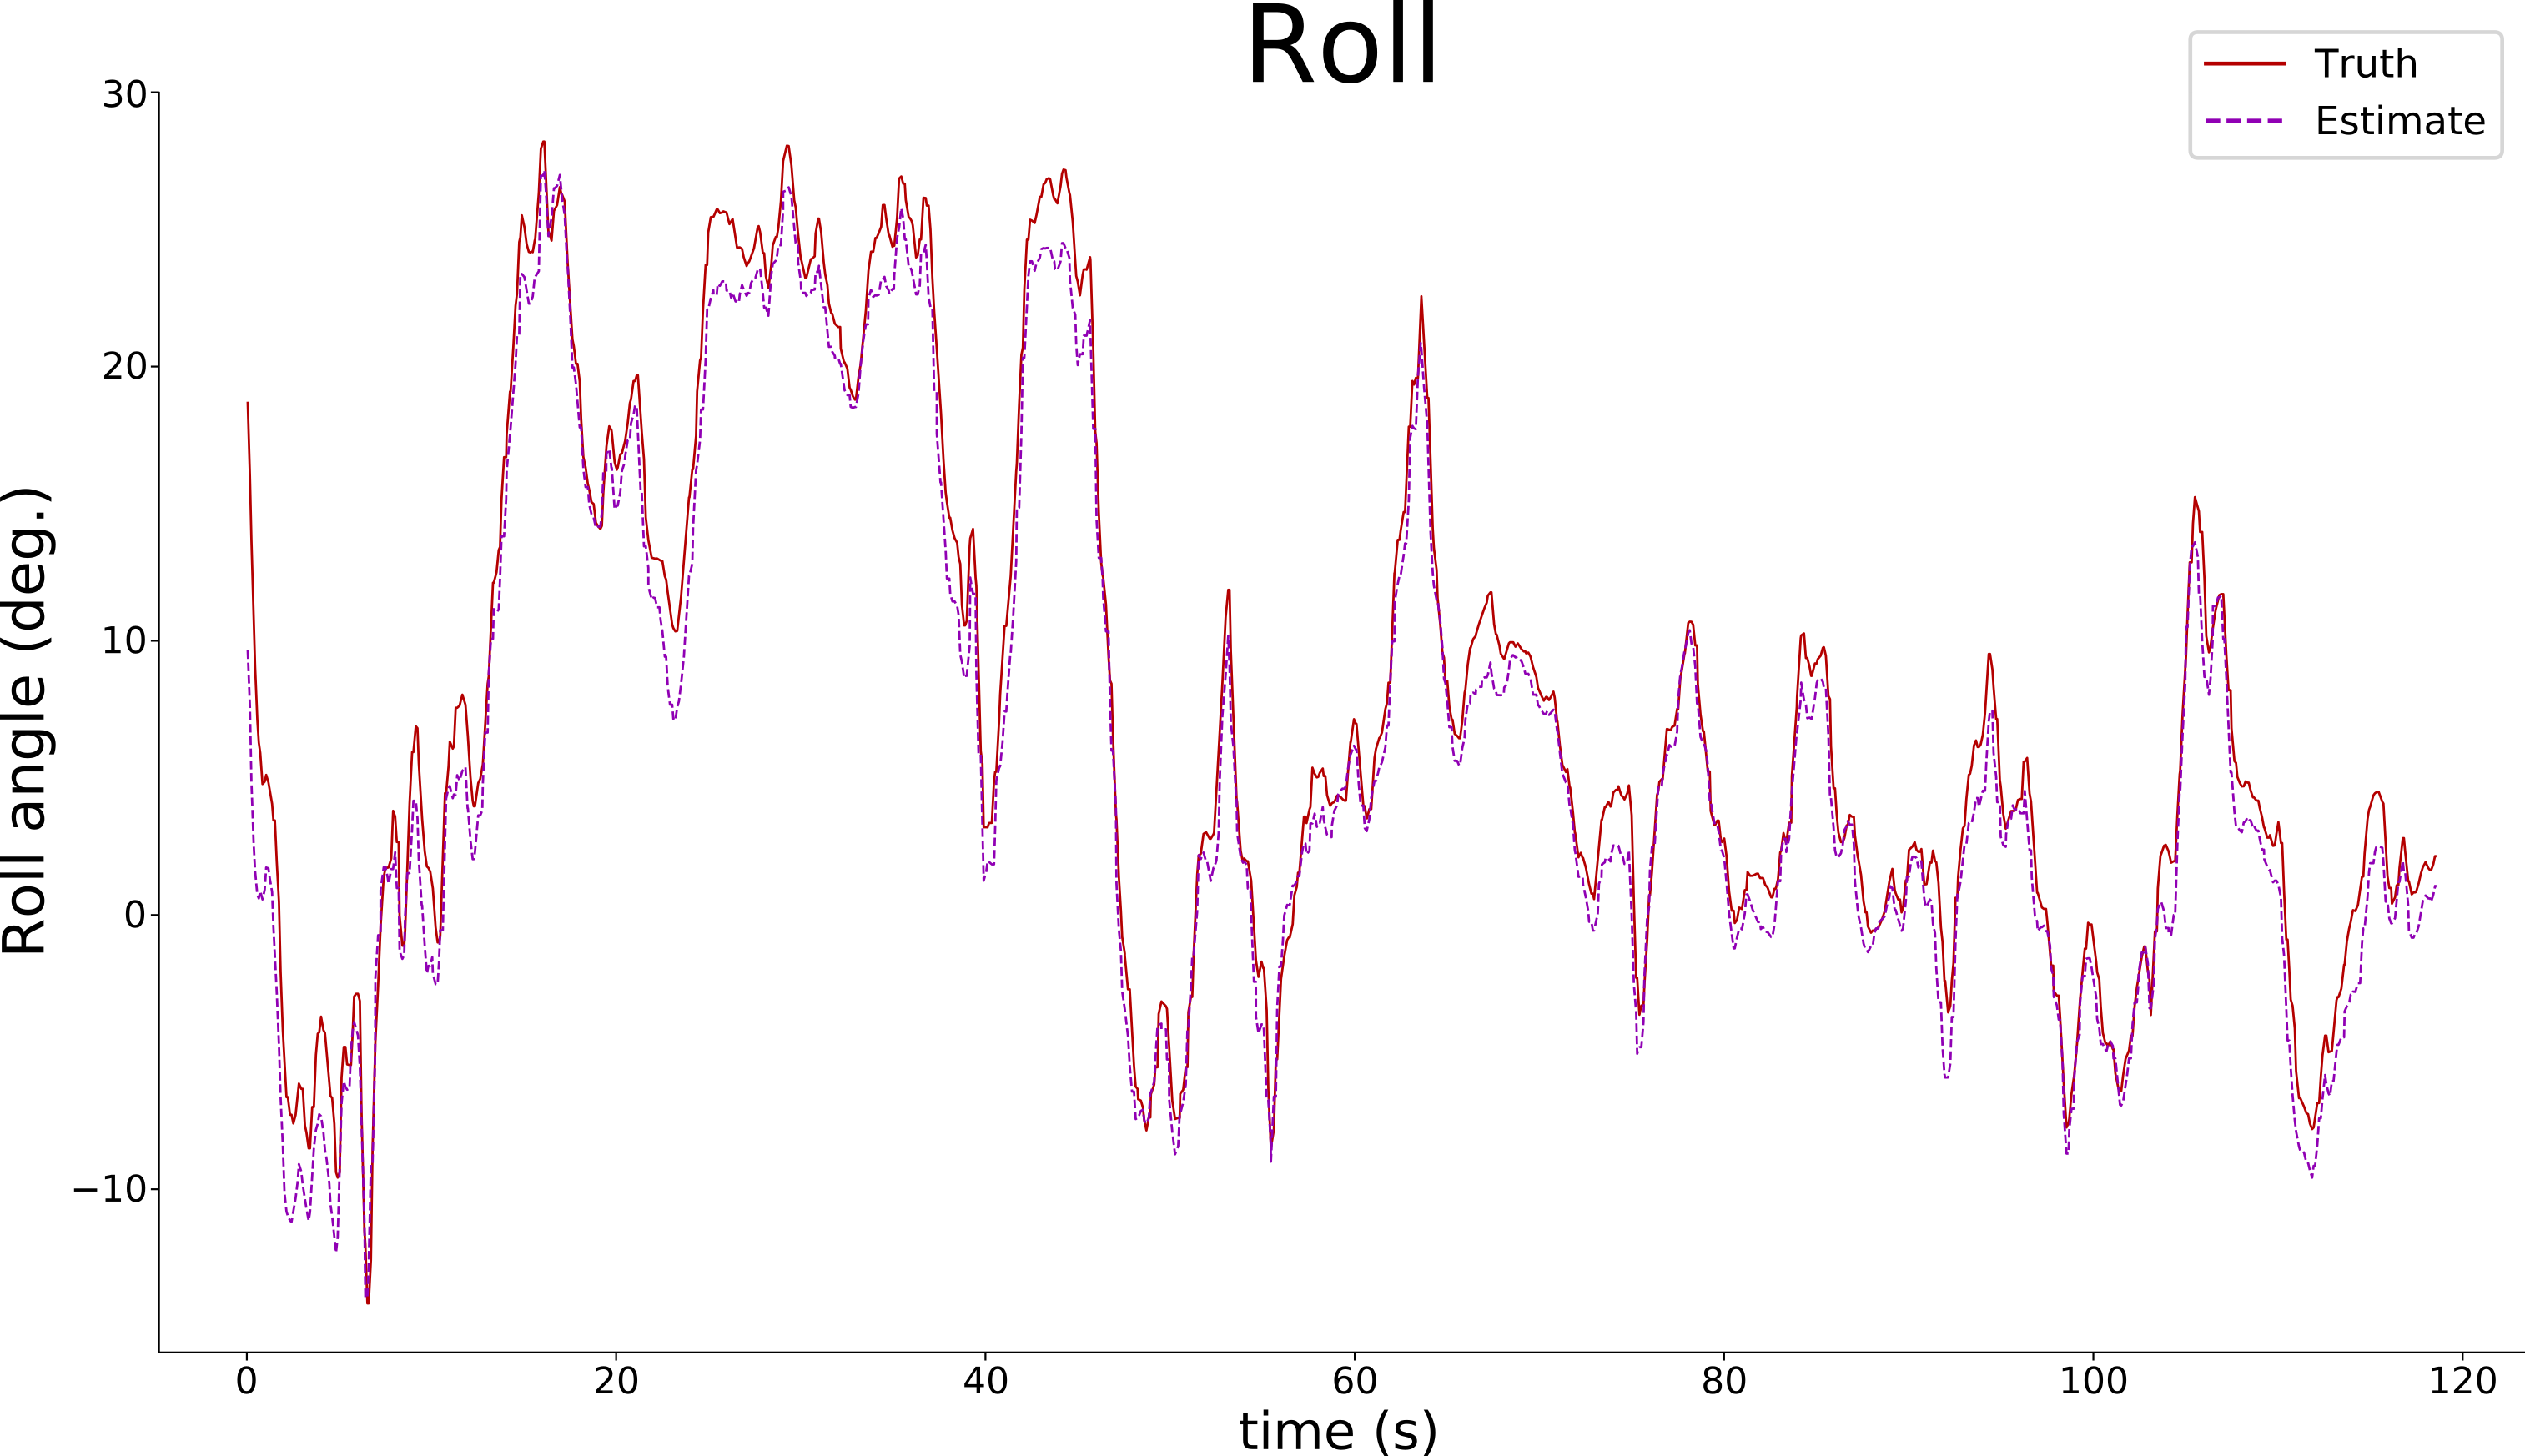
\includegraphics[width=\columnwidth]{figures/hardware_roll_plot}
	\caption{Plot of roll estimate during a hardware flight test.}
	\label{fig:roll_plot}
\end{figure}

\begin{figure}[hbt]
	\centering
	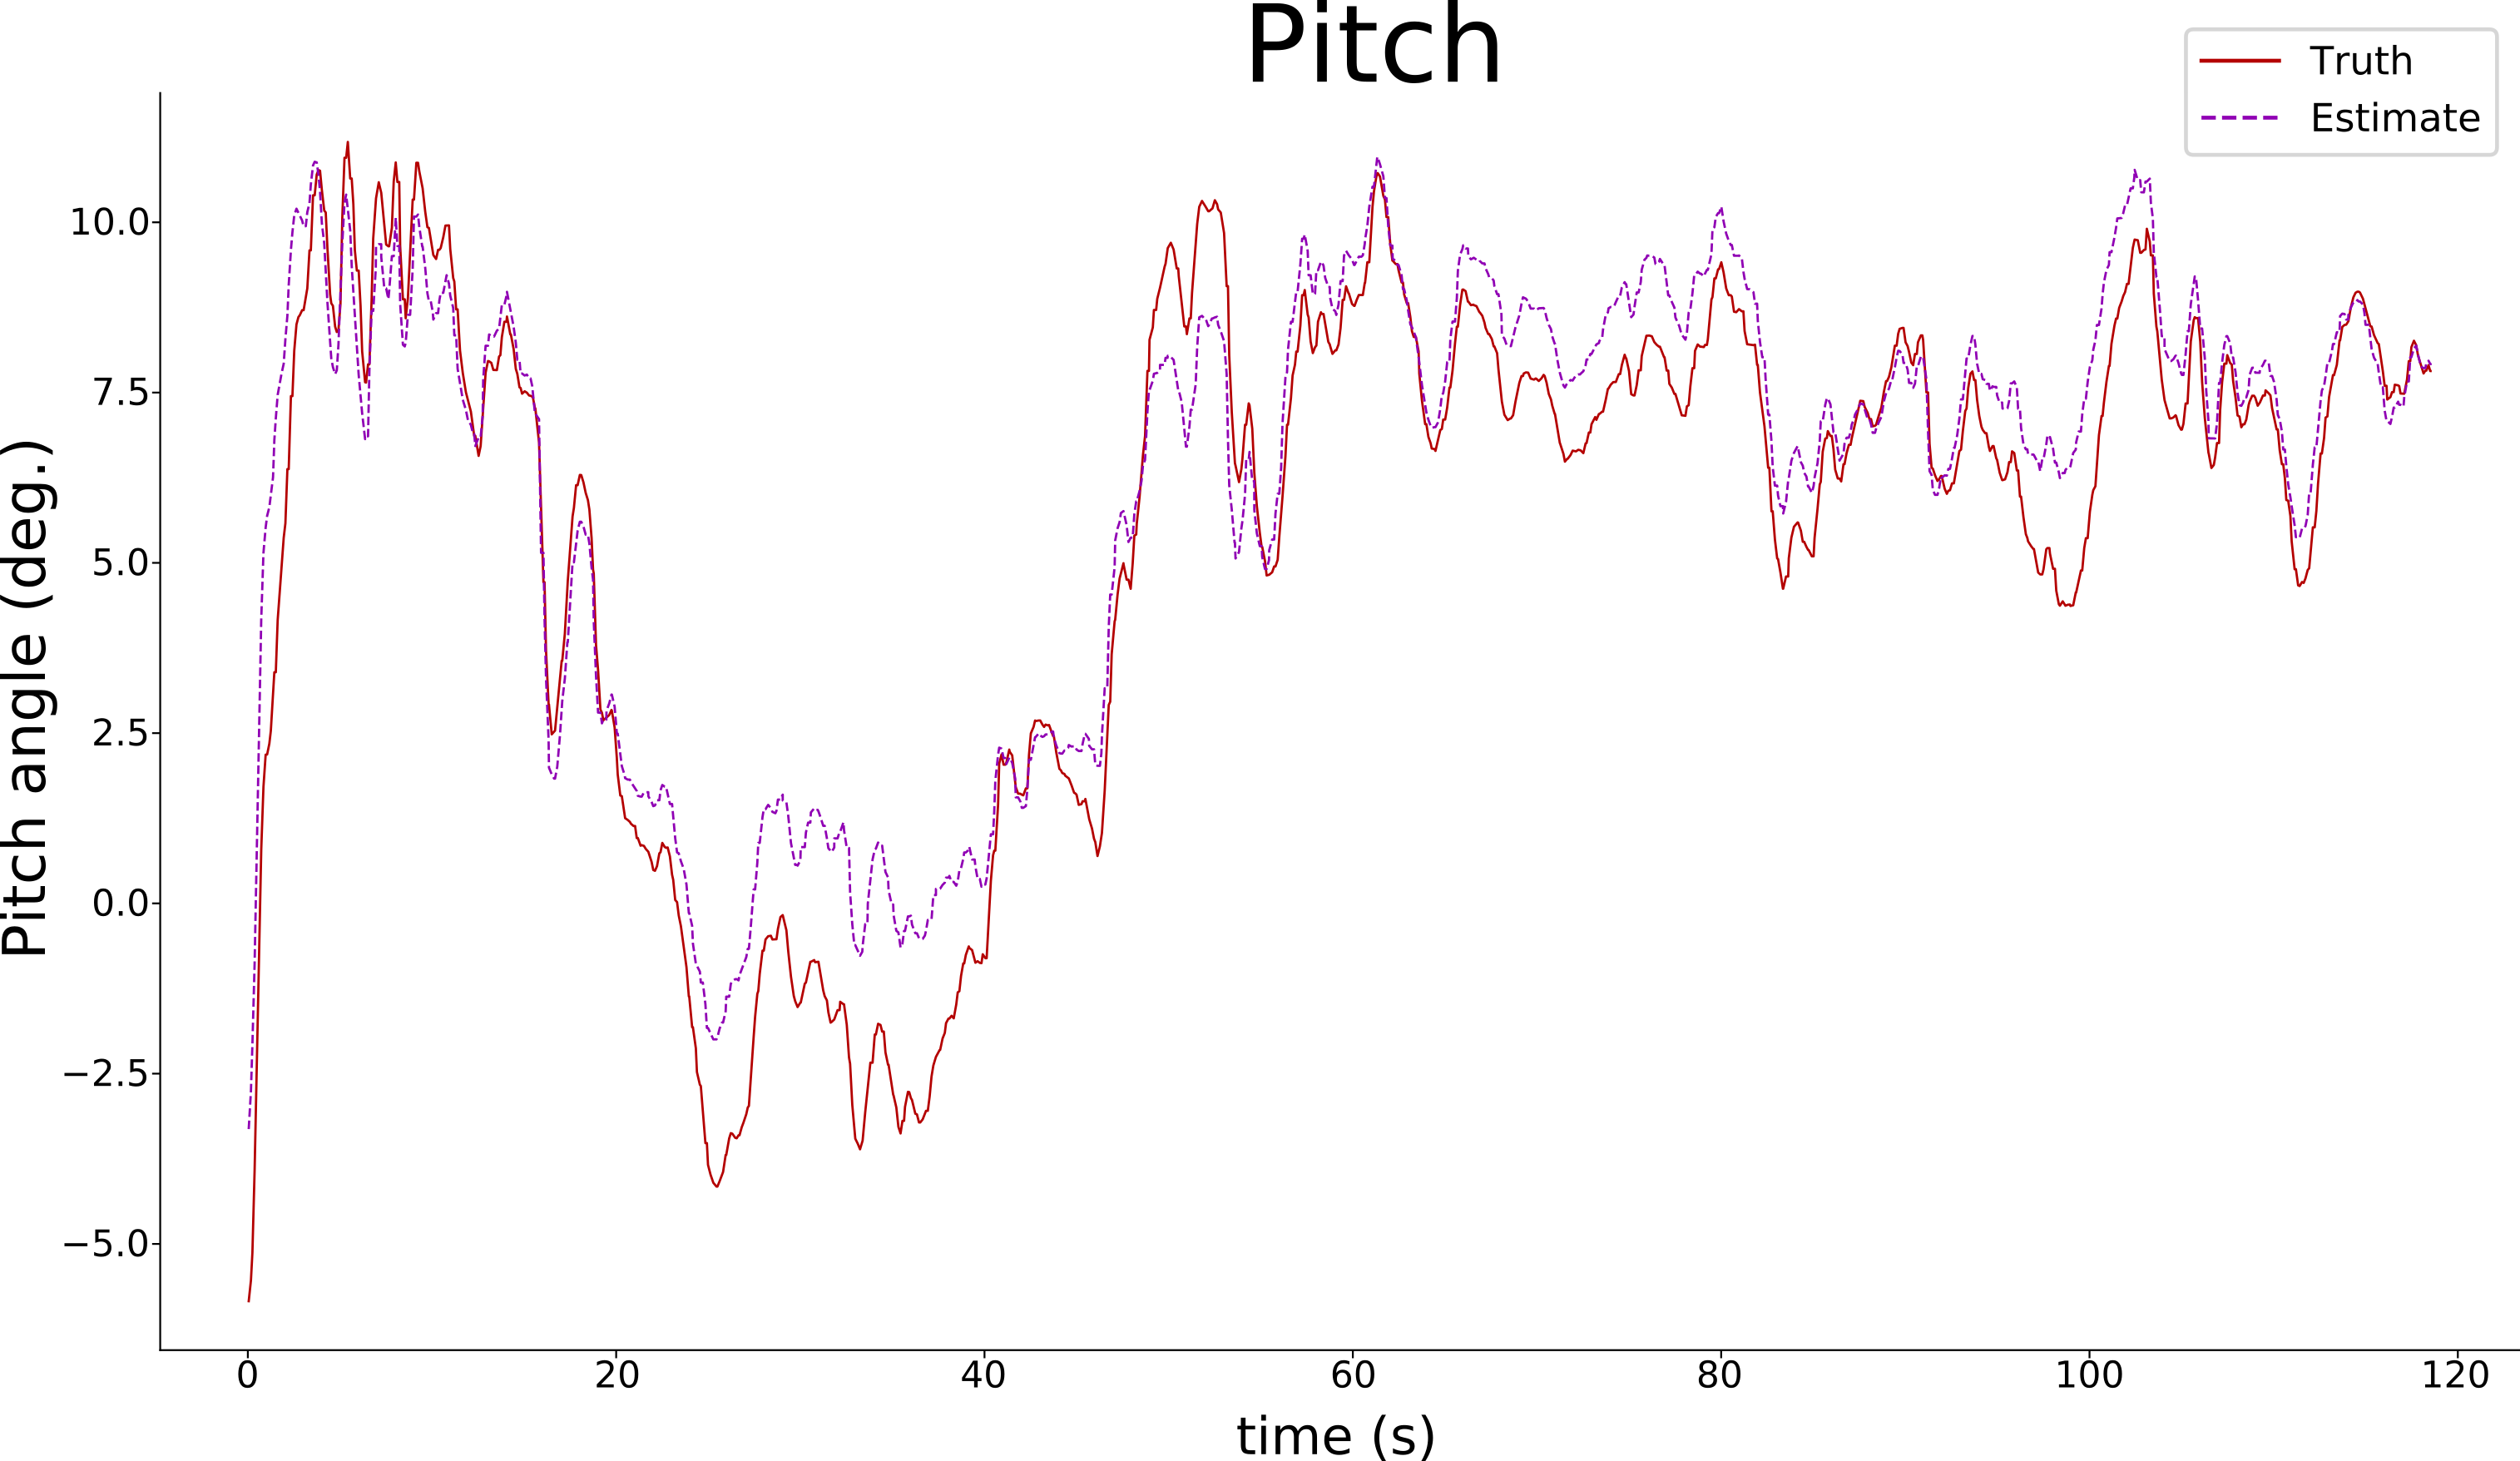
\includegraphics[width=\columnwidth]{figures/hardware_pitch_plot}
	\caption{Plot of pitch estimate during a hardware flight test.}
	\label{fig:pitch_plot}
\end{figure}

\begin{table}[hbt]
  \caption{Self-pose attitude estimation results}
	\label{tab:attitude_results}
	\resizebox{\columnwidth}{!}{%
	\begin{tabular}{c|l|l|}
	\cline{2-3}
	\multicolumn{1}{l|}{}                                                  & \multicolumn{1}{c|}{Roll} & \multicolumn{1}{c|}{Pitch} \\ \hline
	\multicolumn{1}{|c|}{Mean Squared Error (deg)} & 3.067                                             & 1.476                                              \\ \hline
	\multicolumn{1}{|c|}{Average Error (deg)}      & 1.277                                            & -0.655                                              \\ \hline
	\end{tabular}
	}
\end{table}

% Results and comparisons!

% !TEX root=../master.tex
\chapter{GPS-Denied Relative-Pose Estimation}
\label{ch:relative_pose} 

%% TODO: Add related works here
\section{Background and related works}
With each vehicle estimating its own self-pose and body frame velocity, the next step is to estimate the line of sight (LOS) vector between the two vehicles, represented by $\p_{\TwrtH}^\hb$ in \eqref{eq:target_rel_pos}. 
In order to estimate the relative pose between the two vehicles, we assume that the handoff vehicle is receiving measurements of the range between the two vehicles, given by $\xyrange$ where $\xyrange = \norm{\losxy}$.
Because we are measuring the magnitude of the line-of-sight vector, the remaining unknown aspects of the relative pose are the bearing of the LOS vector in the handoff vehicle's navigation frame and the relative heading between the two vehicles. 
We focus primarily on estimating the bearing of the LOS vector, which we represent as $\bearing$. 
We assume that each vehicle is using a calibrated magnetometer that produces a noisy, yet reasonable estimate of global heading, allowing the handoff vehicle to compute the relative heading between the two vehicles, $\relpsifull$.
In \cite{BaiBeard16}, He Bai et al. offer a solution to a similar problem, where the position between the two vehicles is measured and the heading between the two vehicles is estimated using a bank of Kalman Filters. 
We follow a similar approach by using a particle filter to estimate the bearing of the LOS vector, but with a reduced memory and computation footprint.

Agostino Martinelli et al. also offer an observability analysis of estimating the relative pose with a range measurement, showing that the relative pose is observable given that both vehicles have non-zero velocity \cite{MartinelliSiegward05}. 
While the analysis in \cite{MartinelliSiegward05} was performed with 2-dimensional ground robots, we decouple the 3-dimensional problem into relative height and relative position in the $xy$-plane, effectively reducing the bearing estimation to a 2D problem, allowing us to benefit from the observability result. 

\section{State definition}
The goal of the filter is to estimate $\losxy$ measurements of the range between the two vehicles and measurements of each vehicle's altitude.
Because we receive measurements of range directly, we reparameterize $\losxy$ by using polar coordinates for the $xy$-plane. 
This polar-coordinate reparameterization is represented by $\los$, according to
\begin{equation}
    \los = \begin{pmatrix}
    \xyrange \\ \bearing \\ \relzfull
    \end{pmatrix} \;,
\end{equation}
where $\bearing$ is the bearing angle of the LOS vector in the $xy$-plane and $\relzfull$ is the difference in altitude between the handoff and tracking UAVs, given by $z_t - z_h$.

In addition to estimating the LOS vector, we also include the relative heading as a state in the filter to improve upon the noisy measurements from the magnetometers.
Accordingly, the state for the filter becomes
\begin{equation} \label{eq:pf_state}
    \x = \begin{pmatrix} \xyrange \\ \bearing \\ \relzfull \\ \relpsifull \end{pmatrix}
\end{equation} \;.

\section{State Dynamics}
Before discussing the actual filter implementation, it is instructive to first investigate the dynamics of the state, $\x$.
Although the filter uses a polar-coordinate definition for the LOS vector, we begin the derivation of the dynamics using a Cartesian representation for simplicity.

Let $\losxy$ represent the Cartesian LOS vector from the handoff vehicle to the tracking vehicle in the handoff vehicle-1 frame, given by
\begin{align}
    \losxy &= \Rot{i}{\hv}\p_{\TwrtH}^{i} \;,
\end{align}
where $\p_{\TwrtH}^i$ is a NED vector representing the position of the tracking vehicle relative to the handoff vehicle in the inertial frame.

Taking the time derivative, we get
\begin{align}
    \losxy[\dot] &= \Rotdot{i}{\hv}\p_{\TwrtH}^{i} +
                  \Rot{i}{\hv}\dot{\p}_{\TwrtH}^{i} \\
    \label{eq:vhhv}
    &= \Rotdot{i}{\hv}\p_{\TwrtH}^{i} +
       \Rot{\tv}{\hv}\Rot{\tb}{\tv}\vel_{\TwrtI}^{\tb} -
       \Rot{\hb}{\hv}\vel_{\HwrtI}^{\hb} \\
    &= -\skewmat{\angvel_{\HVwrtI}^\hv}\Rot{i}{\hv}\p_{\TwrtH}^{i} +
       \Rot{\tv}{\hv}\Rot{\tb}{\tv}\vel_{\TwrtI}^{\tb} -
       \Rot{\hb}{\hv}\vel_{\HwrtI}^{\hb} \\
    &= -\skewmat{\angvel_{\HVwrtI}^\hv}\p_{\TwrtH}^\hv +
       \Rot{\tv}{\hv}\Rot{\tb}{\tv}\vel_{\TwrtI}^{\tb} -
       \Rot{\hb}{\hv}\vel_{\HwrtI}^{\hb} \\
    \label{eq:losdot}
    &= -\skewmat{\angvel_{\HVwrtI}^\hv}\losxy + \vel_{\TwrtH}^\hv \;,
\end{align}
where $\skewmat{\cdot}$ is the skew-symmetric matrix operator such
\begin{equation}
  \skewmat{\vect{a}} \triangleq \begin{bmatrix}
                                0 & -a_z & a_y \\
                                a_z & 0 & -a_x \\
                                -a_y & a_x & 0
                                \end{bmatrix}.
\end{equation}
Also, because the handoff vehicle-1 frame only differs from the inertial frame by a $z$ rotation, $\angvel_{\HVwrtI}^\hv$ can be interpreted as the rotation about the $z$ axis of the vehicle-1 frame, given by
\begin{align}
    \label{eq:omega_z}
    \angvel_{\HVwrtI}^\hv &= \e_3\e_3^\transpose\Rot{\hb}{\hv}\angvel_{\HBwrtI}^\hb \\
    &= \angvel_{\text{h}z}^\hv \;.
\end{align}

The dynamic equation in \eqref{eq:losdot} essentially has two parts.
The first half of the sum represents the rotational part, which is the relative motion induced by the handoff vehicle's yawing motion.
The second half of the sum represents the translational part, caused by the relative linear velocity between the two vehicles.
For simplicity, we will consider the effect that each of the components have on the polar-coordinate representation separately, then combine them for a final result.

If the handoff vehicle had no rotational motion (e.g. $\angvel_{\text{h}z}^\hv = \mathbf{0}$, the time derivative of the LOS vector would depend entirely on $\vel_{\TwrtH}^\hv$.
The velocity vector can be thought of as having two components---one that is parallel to the LOS vector, representing the radial motion of the tracking vehicle towards and away from the handoff vehicle, and one that is orthogonal to the LOS vector, representing the tangential motion about the current radius at which the tracking vehicle resides (see Figure~\ref{fig:rel_pose_vectors}).

\begin{figure}[hbt]
    \centering
    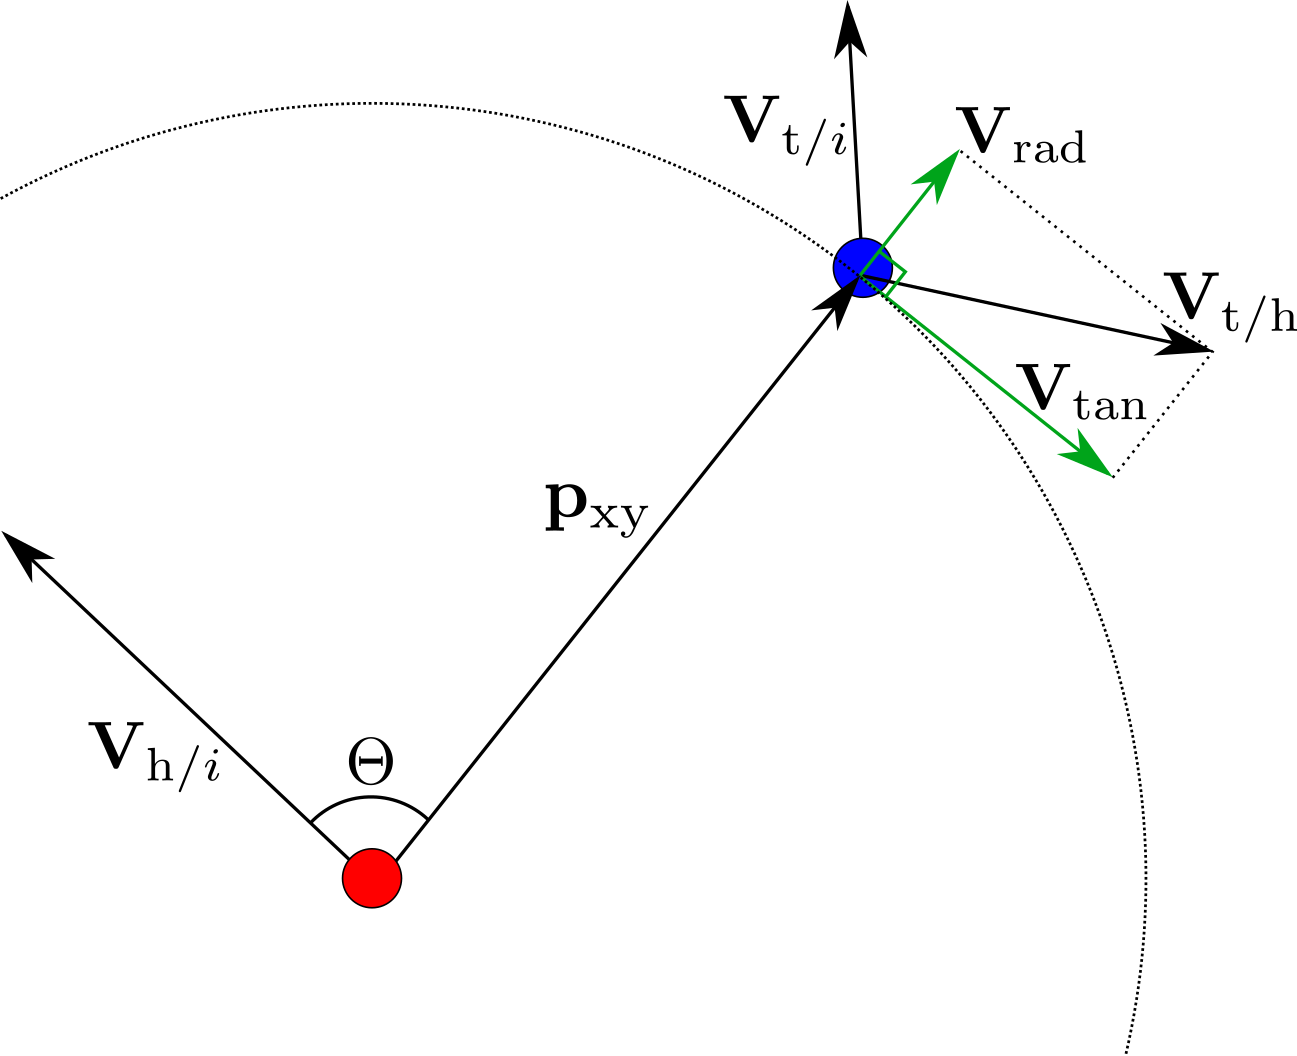
\includegraphics[width=0.5\columnwidth]{figures/rel_pose_vectors}
    \caption{Depiction of relative pose vectors.}
    \label{fig:rel_pose_vectors}
\end{figure}

Using these components, it is simple to derive the polar coordinate dynamics.
The change in range, $\xyrange[\dot]$, depends directly on the radial component according to
\begin{align}
    \xyrange[\dot] &= \norm{\vel_\text{rad}} \\
        &= \frac{\vel_{\TwrtH}^\hv \cdot \pxy}{\norm{\pxy}} \label{eq:rhodot_projection} \\
        &= \vel_{\TwrtH}^\hv \cdot \begin{pmatrix} \cos\bearing \\ \sin\bearing \\ 0 \end{pmatrix} \;,
\end{align}
where $\pxy$ represents the LOS projected onto the $xy$-plane.

The change in bearing can be derived from the tangential component according to
\begin{align}
    \bearing[\dot] &= \frac{\norm{\vel_\text{tan}}}{\xyrange} \\
        &= \frac{1}{\xyrange} \vel_{\TwrtH}^\hv \cdot \begin{pmatrix} -\sin\bearing \\ \cos\bearing \\ 0 \end{pmatrix} \;.
\end{align}
The $z$ component of $\los$ is simply dependent upon the $z$ component of $\vel_{\TwrtH}^\hv$ such that
\begin{equation}
    \relzfull[\dot] = \e_3 \cdot \vel_{\TwrtH}^\hv \;.
\end{equation}

The rotational part of \eqref{eq:losdot} only effects the $\bearing$ dynamics, so the full dynamics of $\los$ become
\begin{align}
    \los[\dot] &= \begin{pmatrix}
        \begin{bmatrix} \cos\bearing & \sin\bearing & 0 \end{bmatrix} \vel_{\TwrtH}^\hv   \\
        \frac{1}{\xyrange} \begin{bmatrix} -\sin\bearing & \cos\bearing & 0 \end{bmatrix} \vel_{\TwrtH}^\hv  - \angvel_{\text{h}z}^\hv \\
        \e_3 \cdot \vel_{\TwrtH}^\hv
        \end{pmatrix} \\
    &= \begin{pmatrix}
    \cos\bearing & \sin\bearing & 0 \\
    -\frac{1}{\xyrange}\sin\bearing & \frac{1}{\xyrange}\cos\bearing & 0 \\
    0 & 0 & 1
    \end{pmatrix} \vel_{\TwrtH}^\hv - \begin{pmatrix} 0 \\ \angvel_{\text{h}z}^\hv \\ 0 \end{pmatrix} \;.
\end{align}

Finally, the dynamics for $\relpsifull$ are simply the difference between the two vehicles' rotation about the inertial $z$ axis, given by
\begin{equation}
    \relpsifull[\dot] = \angvel_{\text{t}z}^\tv - \angvel_{\text{h}z}^\hv \;.
\end{equation}

Accordingly, the time derivative of the filter state, $\x$, becomes
\begin{align} \label{eq:pf_xdot}
\xdot &= \begin{pmatrix}
        \begin{bmatrix} \cos\bearing & \sin\bearing & 0 \end{bmatrix} \vel_{\TwrtH}^\hv   \\
        \frac{1}{\xyrange} \begin{bmatrix} -\sin\bearing & \cos\bearing & 0 \end{bmatrix} \vel_{\TwrtH}^\hv  - \angvel_{\text{h}z}^\hv \\
        \e_3 \cdot \vel_{\TwrtH}^\hv \\
        \angvel_{\text{t}z}^\tv - \angvel_{\text{h}z}^\hv
        \end{pmatrix} \;.
\end{align}

\section{Filter choice}

% - Problem lends itself to particle filter approach
With measurements of the relative heading, relative altitude, and range between the two vehicles, the main goal of the relative pose estimator is to determine the correct value for $\bearing$, the bearing angle of the line of sight (LOS) vector between the two vehicles in the handoff vehicle-1 frame.

This angle is not directly observable with a single time step because we only receive the magnitude of the LOS vector.
Between two measurements, however, we can use the change in range to narrow the possible values of $\bearing$ down to two options.
As seen in \eqref{eq:rhodot_projection}, $\xyrange[\dot]$ can be expressed as the magnitude of the relative velocity projected onto the LOS vector in the $xy$-plane, according to
\begin{align}
    \xyrange[\dot] &= \frac{\pxy \cdot \vrelfull}{\norm{\pxy}}\\
    &= \frac{\norm{\pxy}\norm{\vrelfull}\cos\beta}{\norm{\pxy}}\\
    &= \norm{\vrelfull}\cos\beta
    \;,
\end{align}
where $\beta$ is the angle between the relative velocity vector and the LOS vector, as seen in Figure~\ref{fig:rhodot_vectors}.

\begin{figure}[hbt]
    \centering
    \includegraphics[width=0.5\columnwidth]{figures/rhodot_vectors}
    \caption{Depiction of two possible $\bearing$ values based on $\xyrange[\dot]$}
    \label{fig:rhodot_vectors}
\end{figure}

Solving for $\beta$, we get
\begin{equation}
    \beta = \pm \acos\left(\frac{\xyrange[\dot]}{\norm{\vrelfull}}\right) \;,
\end{equation}
which means that there are two solutions representing valid values for $\bearing$.
Due to this ambiguity of solutions based on subsequent measurements of the range, filters that attempt to propagate the estimated state along a continuous trajectory, such as an EKF, are not well suited to this problem.
Accordingly, we decided to use a particle filter to approximate this split distribution of appropriate $\bearing$ values.
Over multiple time steps, one of the two bearing distributions will move in a direction that coincides with the dynamics while the other will not, allowing us to determine the correct value probabilistically.

\section{Particle filter implementation}
The particle filter consists of $N$ particles, each with a state and dynamics given by Equations~\eqref{eq:pf_state} and \eqref{eq:pf_xdot} respectively.

The inputs to the system are
\begin{equation}
    \u = \pmat{\angvel_h \\ \angvel_t \\ \vhb \\ \vtb \\ \phi_h \\ \theta_h \\ \phi_t \\ \theta_t} \;,
\end{equation}
where $\angvel_h$ and $\angvel_t$ represent angular velocities from the IMU, $\vhb$ and $\vtb$ are body-frame airspeed vectors from the self-pose filter computed according to \eqref{eq:vair_vec}, and $\phi$ and $\theta$ angles are the estimated roll and pitch angles from the self-pose filter, respectively.

At each time step the state of each particle is propagated according to the dynamics in Equation~\eqref{eq:pf_xdot} with
\begin{align}
    \vrelfull &=\Rot{\tv}{\hv}\Rot{\tb}{\tv}\vel_{\TwrtI}^{\tb} -
       \Rot{\hb}{\hv}\vel_{\HwrtI}^{\hb} \\
       &= \Rot{\relpsi}{}\Rot{\theta_t}{}\Rot{\phi_t}{}\vel_{\TwrtI}^{\tb} -
       \Rot{\theta_h}{}\Rot{\phi_h}{}\vel_{\HwrtI}^{\hb}\;,
\end{align}
and
\begin{align}
    \angvel_{jz}^{j\text{v1}} &=
    \e_3\e_3^\transpose\Rot{j\text{b}}{j\text{v1}}\angvel_{j\text{b}/i}^{j\text{b}} \\
    &= \e_3\e_3^\transpose\Rot{j\theta}{}\Rot{j\phi}{}\angvel_{j\text{b}/i}^{j\text{b}}\;,
\end{align}
where
\begin{align}
        \label{eq:R_psi}
    \Rot{\psi}{} &= \pmat{
        \cos\psi & -\sin\psi & 0 \\
        \sin\psi & \cos\psi & 0 \\
        0 & 0 & 1
    }\;, \\
        \label{eq:R_theta}
    \Rot{\theta}{} &= \pmat{
        \cos\theta & 0 & \sin\theta \\
        0 & 1 & 0 \\
        -\sin\theta & 0 & \cos\theta
    }\;, \\
        \label{eq:R_phi}
    \Rot{\phi}{} &= \pmat{
        1 & 0 & 0 \\
        0 & \cos\phi & -\sin\phi \\
        0 & \sin\phi & \cos\phi
    }\;,
\end{align}
and
\begin{equation}
    \e_3 = \pmat{0 \\ 0\\ 1}\;.
\end{equation}

% - Define measurements and measurement model
The measurement for the filter is composed of range, relative altitude, and relative heading and is defined as
\begin{equation}
    \y = \pmat{\range \\  \relz \\ \relpsi}\;.
\end{equation}
Note that the $[\;]_\text{rel}$ notation is used here in place of $[\;]_{\TwrtH}^{\hv}$ for notational simplicity.

Using the current estimated state of each particle, $\hat{\x}^i_k$, at time step $k$, we construct an estimated measurement, $\y[\hat]$, such that
\begin{equation}
    \y[\hat]^i_k = \pmat{\sqrt{{\xyrange[\hat]}^2 + {\relz[\hat]}^2} \\ \relz[\hat] \\ \relpsi[\hat]}\;.
\end{equation}

Let $\mathbb{Y}\sim \mathcal{N}(\y, \Q)$ represent a multivariate Gaussian distribution centered about $\y$ with covariance $\Q$ and let $f_{\mathbb{Y}}$ be the log PDF of $\mathbb{Y}$.
The weight for each particle is obtained using the softmax function according to
\begin{equation} \label{eq:softmax}
    w^i_k = \frac{\exp\left(f_\mathbb{Y}(\y[\hat]^i_k)\right)}{\sum\limits_{j=1}^{N}\exp\left(f_\mathbb{Y}(\y[\hat]^j_k)\right)}\;,
\end{equation}
where $w^i_k$ represents the weight of the $i$-th particle at time step $k$.
In practice, we use the ``log-sum-exp trick'' for computational stability by subtracting off the maximum log probability, according to
\begin{equation} \label{eq:logsumexp}
    w^i_k = \frac{\exp\left(f_\mathbb{Y}(\y[\hat]^i_k) - \max\limits_l f_\mathbb{Y}(\y[\hat]^l_k) \right)}
    {\sum\limits_{j=1}^{N}\exp\left(f_\mathbb{Y}(\y[\hat]^j_k) - \max\limits_l f_\mathbb{Y}(\y[\hat]^l_k) \right)}\;.
\end{equation}
Equations~\eqref{eq:softmax}~and~\eqref{eq:logsumexp} are mathematically equivalent, but subtracting off the maximum before exponentiating the log probabilities reduces the chance of underflow for low-probability values.

The particles are then resampled with probability proportional to their weights.
However, to reduce particle deprivation and minimize the chance of throwing away good particles, we employ two techniques.
The first is low-variance resampling, which is described in detail in \cite{ThrunBurgardFox06}.
Because the resampling step is a stochastic process, it is possible to lose good particles simply by not resampling them.
Low-variance resampling helps to deal with this challenge by using a random seed to sample from the particles in a more systematic fashion, reducing the probability that particles with higher weights will be lost.

The second technique employed is selective resampling based on the number of effective particles.
This method is described in \cite{GrisettiStachnissBurgard09} and involves resampling only when the number of effective particles drops below a set threshold, such as $\frac{2N}{3}$.
The number of effective particles is estimated by
\begin{equation}
    N_\text{eff}={\frac{1}{\sum\limits_{i=1}^{N} {(w^{i})}^{2}}}\;,
\end{equation}
and is inversely proportional to the variance of the weights.
If the particles very closely match the true distribution, then the particles will have similar weights and low variance.
This would cause $N_\text{eff}$ to be high, which would allow the system to propagate the distribution without the need to resample.
Over time, if the particles became more diffused and the variance of the weights increases, then the number of effective particles would drop below the threshold and new particles would be resampled in an effort to improve the current approximation of the distribution.
By resampling only when $N_\text{eff}$ is below the threshold, the chance of eliminating good particles is reduced.

In order to perform selective resampling, it is important to update the weights of the particles at each successive time step between resampling.
This can be done according to
\begin{equation}
    w^i_{k+1} = \eta w^i_k f_\mathbb{Y}(\y[\hat]^i_{k+1})\;,
\end{equation}
where $\eta$ is a normalization constant.
After the particles are resampled, all weights are reset to $\frac{1}{N}$.

\section{Results} \label{sec:rel_pose_results}
The relative pose particle filter was tested in simulation using simulated IMU, airspeed, altitude, magnetometer, and range measurements, each with added Gaussian noise.
In general, the relative pose estimate converged quickly and provided a sufficiently accurate estimate for the handoff UAV to locate the target and insert into a similar orbit.
As expected, the particle filter displayed a bimodal distribution before converging onto the proper bearing angle as shown in Figure~\ref{fig:particle_filter}.

\begin{figure}[hbt]
  \centering
  \includegraphics[width=\columnwidth]{figures/particle_filter}
  \caption{\textit{Top left}: particles are initialized uniformly across all bearing angles; \textit{Top right}: particles begin to split into a bimodal distribution; \textit{Bottom left}: particles are grouped in two distinct clusters, but with more particle density around the correct bearing; \textit{Bottom right}: the particles consolidate and center around the true value}
  \label{fig:particle_filter}
\end{figure}

Figure~\ref{fig:theta_convergence} shows the estimate of the bearing diverging slightly, then converging sharply as the particles finally consolidate completely around the correct value.
After the particles consolidate, they remain centered around the true value and the estimate of $\Theta$ tracks well.

\begin{figure}[hbt]
  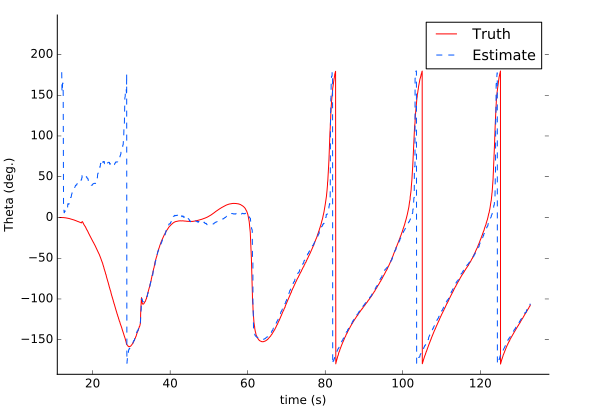
\includegraphics[width=\columnwidth]{figures/Theta_convergence}
  \caption{Plot of $\Theta$ estimate; diverges slightly as particles split into bimodal distribution, then converges sharply as particle consolidate around the true value.}
  \label{fig:theta_convergence}
\end{figure}

\begin{figure}[hbt]
  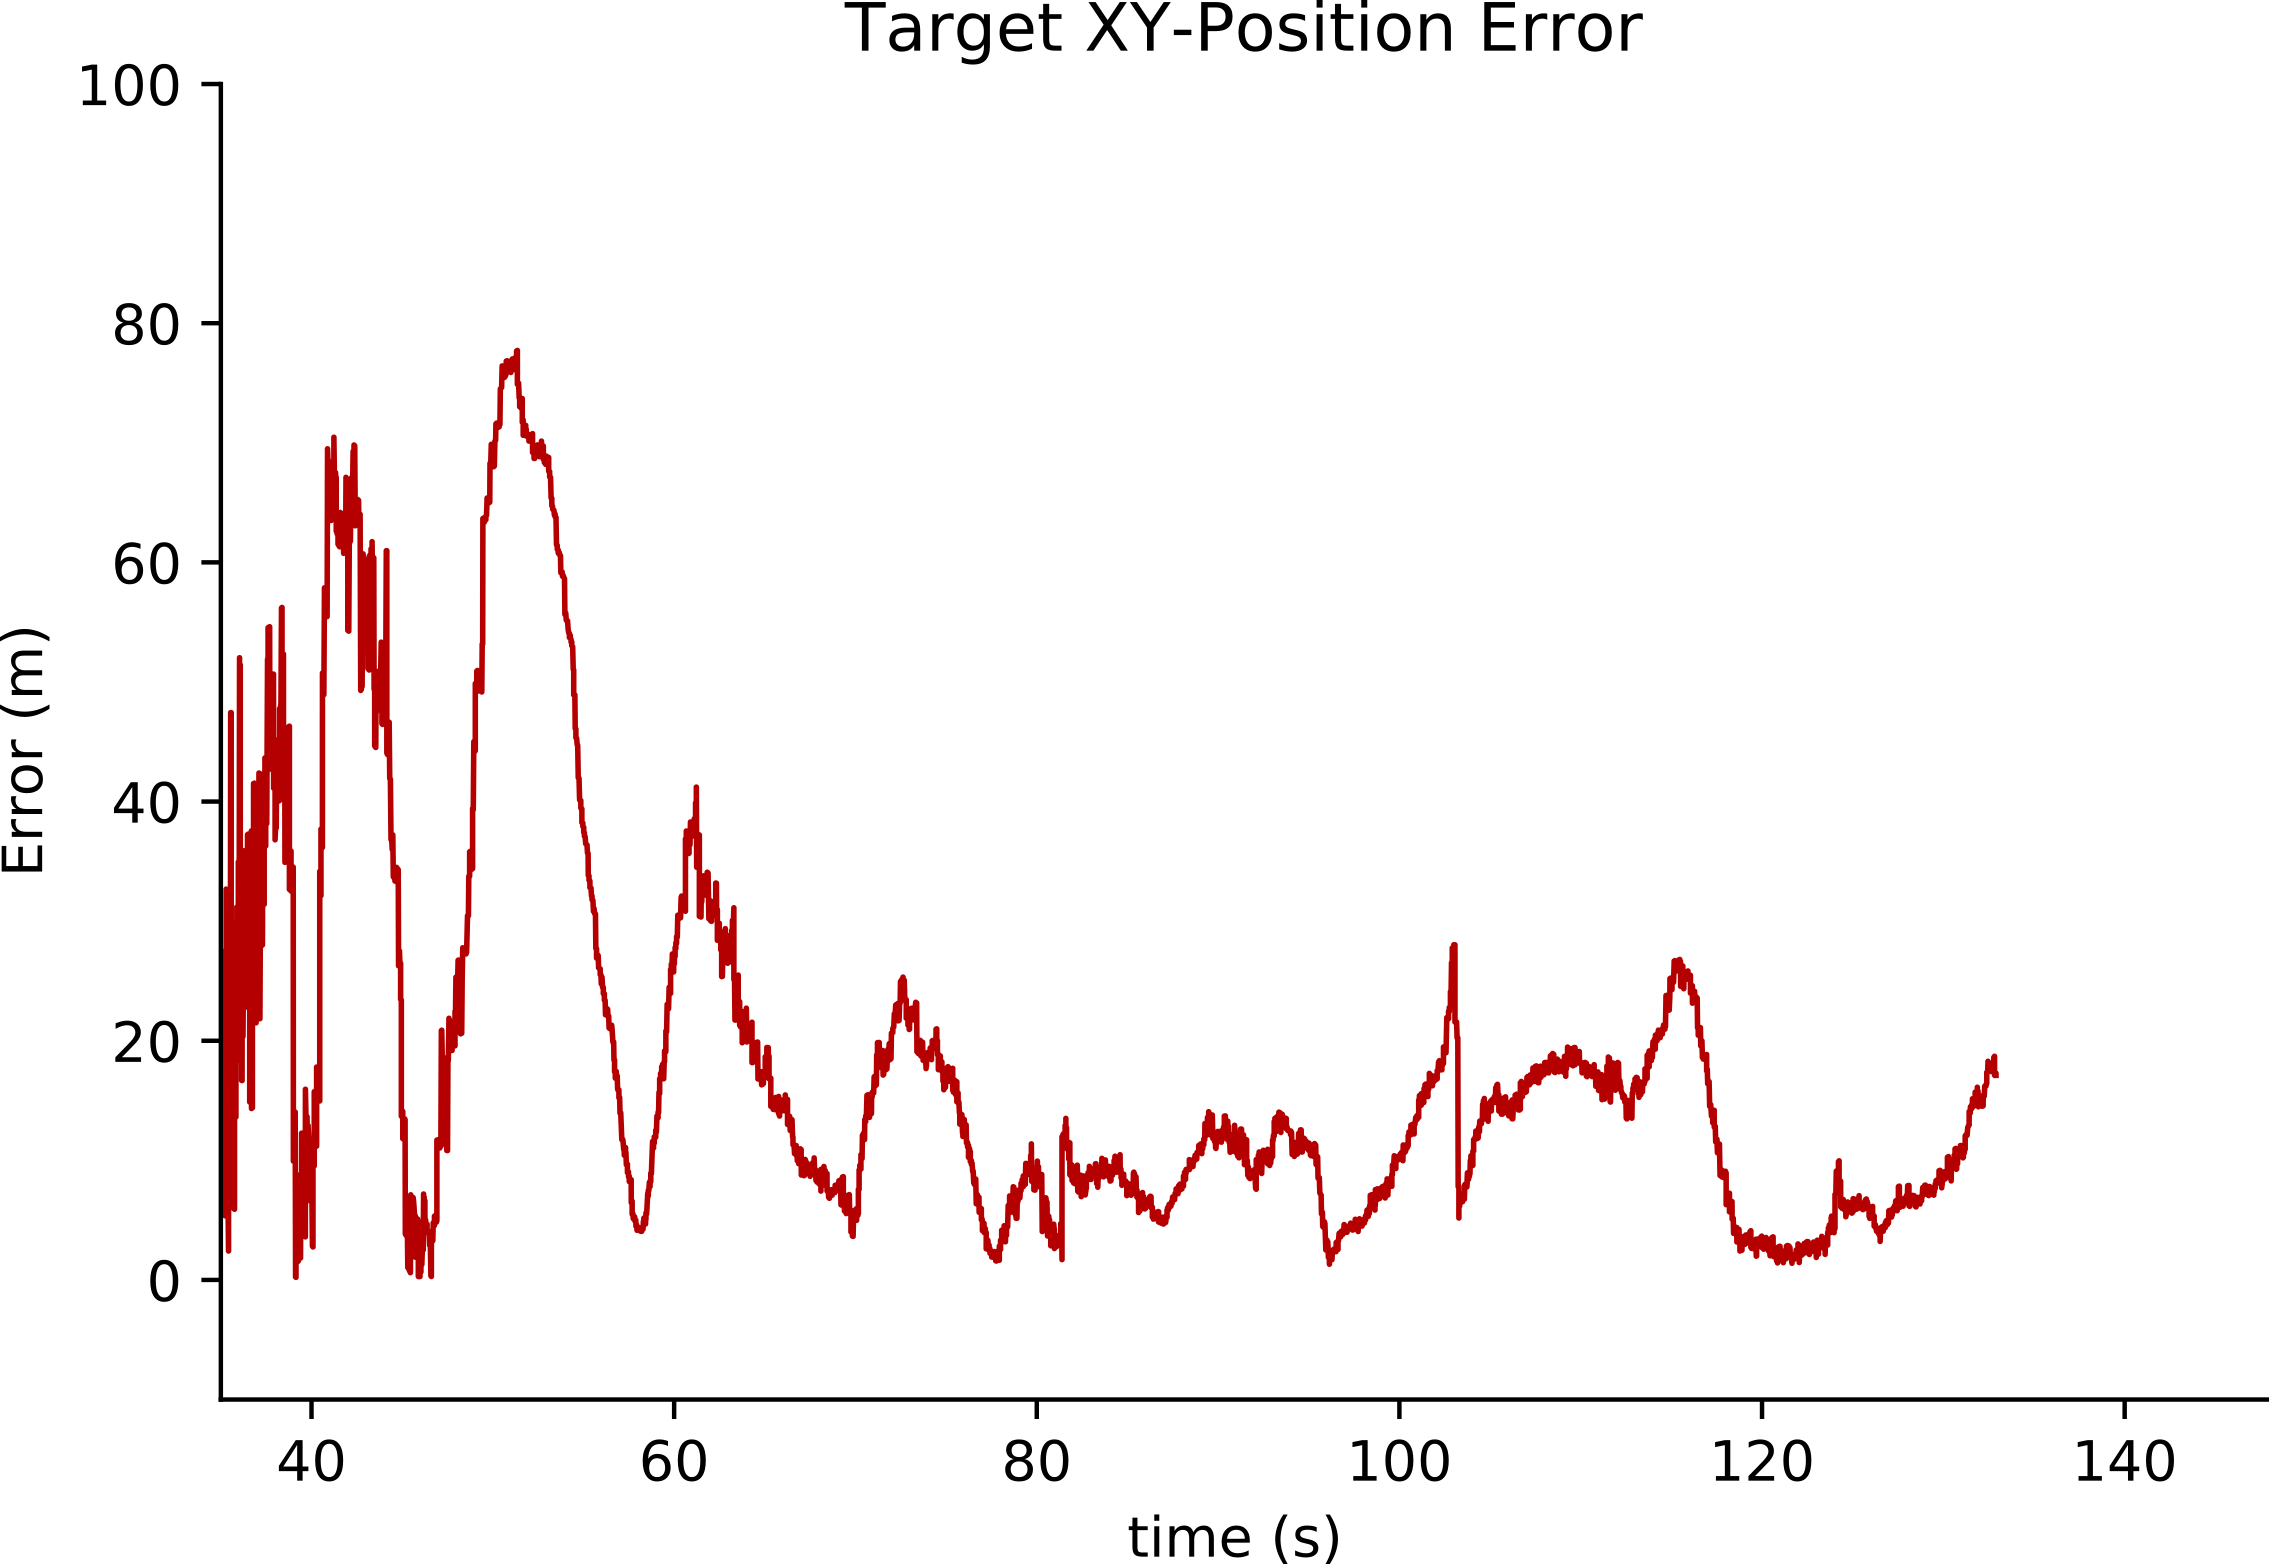
\includegraphics[width=\columnwidth]{figures/target_error}
  \caption{Plot of estimated target $xy$-position error.}
  \label{fig:target_los_error}
\end{figure}

We observed that because the estimated line of sight is parameterized using angle and magnitude and because the range between the two vehicles is often large, small errors in the bearing angle estimate can lead to large errors in the $xy$-plane.
Accordingly, the relative pose estimate is not ideal for obtaining a fine-tuned estimate of the target's position.
However, it does serve it's intended purpose well, providing a reasonable and quickly converging estimate of the relative pose, which allows us to get a good estimate of the target's position to be used in the orbit control.
As seen in Figure~\ref{fig:target_los_error}, after the relative pose estimate begins to converge, the target LOS error can still be as high as 80 meters, but over time, it remains near or below 20 meters.
This level of accuracy is sufficient to locate the target and retain it in the field of view, allowing the handoff UAV to utilize visual information to perform the handoff with greater confidence.


% !TEX root=../master.tex
\chapter{GPS Denied Orbit Control}
\label{ch:orbit_control}
% - interesting because of the GPS denied aspect

Once the handoff vehicle has obtained a reasonable estimate of the relative transform between itself and the tracking UAV, it is equipped to insert itself into a similar orbit about the target.
Because there is no GPS-data available, the orbit control must only use estimates of the target's position and velocity relative to the vehicle.
Initially, the handoff UAV will use the relative pose information to compute the LOS between itself and the target according to Equation~\eqref{eq:target_rel_pos}, but by the time the target handoff is complete, it will need to orbit the target based entirely on visual data.

Another challenge of GPS-denied orbiting is that the vehicle cannot use global waypoints or orbit centers to loiter about the target, but must instead give heading rate or roll commands.
The implementation here assumes the ability to command roll directly, but the derivation for commanding heading rate would be similar.
This section describes the control used to compute appropriate roll commands from the target's relative position and velocity.
We also discuss how we orbit the target using only visual information after the handoff is complete.

\section{Orbit Control}

\subsection{Target relative state}
As previously noted, without GPS, the state of the target must be represented relative to the UAV. We will represent the state of the target as
\begin{equation}
    \x_\tg = \pmat[1.5]{\ptghv \\ \veltghv}\;,
\end{equation}
where the target position represents the line of sight vector frome the UAV to the target and the target velocity represents the motion of the target relative to the UAV.

In the context of the orbit control, it is more intuitive to think of the target as being stationary, with the handoff vehicle moving with some velocity relative to the target.
Accordingly, in the control derivation, we refer to the relative velocity as $\velhtg$, which is just the negative of the target's velocity relative to the UAV, according to
\begin{equation}
    \velhtg = -\veltghv\;.
\end{equation}

Because the target is in motion, a constant radius orbit about the target would take the form of a spiral in the world xy-frame.
Rather than attempting to follow a spiral trajectory in the world frame, we can simplify the problem by controlling the UAV to follow a constant radius orbit in the target relative frame.
The end result is analagous to controlling a constant orbit in the presence of wind.

In order to maintain a constant orbit in the relative frame, the UAV must maintain a $90^\degree$ angle between the relative velocity vector and the line of sight vector to the target.
This angle will be denoted by $\gamma$.
The angle between the x-axis of the vehicle and the line of sight vector to the target will be given by $\az$, which correpsonds with the azimuth of the gimbal.
Figure~\ref{fig:target_relative_vectors} gives a visual representation of these vectors and angles.
\begin{figure}[hbt]
    \centering
    \includegraphics[width=0.5\columnwidth]{figures/target_vel_vectors}
    \caption{Depiction of target relative position, velocity, and related angles.}
    \label{fig:target_relative_vectors}
\end{figure}

\subsection{Control implementation}

The goal of the orbit control is to cause the UAV to fly directly towards the target when it is very far away ($\gamma = 0$) then to gradually drive $\gamma$ to $\frac{\pi}{2}$ when the distance between the target and the UAV approaches the desired orbit radius.

The value of $\gamma$ is computed according to
\begin{equation}
    \gamma = \atantwo\left(\norm{\vel_{\HwrtTG}\cross\ptghv}, \hspace{1em}\vel_{\HwrtTG}\cdot\ptghv\right)\;.
\end{equation}
% While the dot product or cross product alone is sufficient to get the magnitude of the angle between the two vectors, using $\atantwo$ on the quotient of the cross and dot products allows us to determine the proper direction of the angle.

Using the equations for angular velocity in an orbit and the coordinated turn condition for fixed-wing aircraft, we can derive an expression for the desired roll command according to
\begin{align}
    \dot{\gamma} &= \frac{\norm{\vel_{\HwrtTG}}}{R} \\
    &= \frac{g}{\norm{\vel_{\HwrtTG}}}\tan\phi\\
    \label{eq:phi_ff}
    \phiff &= \atan\left(\frac{\norm{\vel_{\HwrtTG}}^2}{gR}\right)\;.
\end{align}

We use the expression in \eqref{eq:phi_ff} as the feed forward term to keep the UAV in a proper orbit.
We also add PD control on $\gamma$ to help the UAV converge onto the proper orbit.
The full roll control becomes
\begin{align}
  \phi_{c} &= \phiff+k_{p}e_{\gamma}+k_{d}\dot{e}_{\gamma}\\
  e_{\gamma} &= \gamma-\gamma_{d}\;.
\end{align}

We want the aircraft to converge to the desired orbit with the appropriate direction (clockwise or counter-clockwise) and radius as quickly as possible. Accordingly, the desired value for $\gamma$ should allow the UAV to fly directly toward or away from the target to quickly approach the desired radius, and then to smoothly transition to the tangential motion of an orbit in the proper direction. To accomplish this, we added an arctangent term to make a smooth transition between the desired range-dependent far-field and near-field behaviors. The expression for the desired $\gamma$ becomes
\begin{equation}
    \gamma_{d} = \lambda\left[\atan\left(-\beta\left(R-R_{d}\right)\right)+\frac{\pi}{2}\right]\;,
\end{equation}
where $\lambda$ represents the direction of the orbit ($+1$ for clockwise and $-1$ for counter-clockwise) and $\beta$ is a constant to control the rate at which $\gamma_d$ should transition from the perpendicular motion to the tangential motion as it approaches the proper orbit.
%% ST: Maybe add something here about choosing beta based on system constraints

\section{Vision-based Orbiting}
 Visual information provides a more reliable measurement of the target's relative position than the relative LOS that is initially used to orbit the target, but it also requires that the UAV maintain the target in the field of view and keep a consistent track in order to receive information.

\subsection{Target position estimation}
Initially the handoff UAV must rely on the information from the relative pose particle filter to estimate the target's position according to
\begin{equation} \label{eq:target_pos_rel}
    \ptghv = \p_{\TwrtH}^\hv + \Rot{\tv}{\hv}\Rot{\tb}{\tv}\p_{\TGwrtT}^\tb\;,
\end{equation}
where $\p_{\TwrtH}^\hv$ and $\Rot{\tv}{\hv}$ are estimates from the particle filter, $\Rot{\tb}{\tv}$ comes from the tracker's complimentary attitude filter, and $\p_{\TGwrtT}^\tb$ is measured by the tracker. Because the value of $\ptghv$ is the product of several estimated and measured values, each with their own noise and uncertainty, it will be relatively noisy. It does contain enough information to help the UAV navigate in the right direction and get the target into the field of view of the camera.
Once the handoff UAV is sufficiently confident that it has found the correct target, it can begin utilize visual information to orbit the target, becoming independent of measurements from the tracking UAV in preparation for tracking UAV's departure.

As long as the handoff UAV can maintain the target in the field of view and keep track of the target visually, the visual information provides a reliable measurment of the relative position of the target.
In order to estimate the target's position, the UAV must transform the line of sight into the proper frame with the proper scale. The handoff UAV's target tracking algorithm will produce the target's position in normalized image plane pixel coordinates of the handoff UAV's camera.

Let
\begin{equation}
    \pimgvec_{\TGwrtH} = \pmat{\pimgvar_x \\ \pimgvar_y \\ 1}
\end{equation}
represent the normalized image coordinates of the target received from the tracker. Normalized image coordinates are normalized by the focal length of the camera in pixels, so that they are independent of the camera intrinsics.
Converting $\pimgvec_{\TGwrtH}$ to a unit vector, we get
\begin{equation}
    \ptg[\check]^c = \frac{\pimgvec_{\TGwrtH}}{\norm{\pimgvec_{\TGwrtH}}}\;.
\end{equation}
We rotate the normalized LOS into the handoff vehicle 1 frame according to
\begin{equation}
    \ptghv[\check] = \Rot{\hb}{\hv}\Rot{g}{\hb}\Rot{c}{g}\ptg[\check]^c\;,
\end{equation}
where $\Rot{c}{g}$ is a fixed rotation given by
\begin{equation}
    \Rot{c}{g} = \pmat{
      0 & 0 & 1 \\ 1 & 0 & 0 \\ 0 & 1 & 0
      }\;,
\end{equation}
$\Rot{g}{\hb}$ can be constructed from the gimbal azimuth ($\az$) and elevation ($\el$) as
\begin{equation}
    \Rot{g}{\hb} = \pmat{\cos\el\cos\az & -\sin\az & \sin\el\cos\az \\
                         \cos\el\sin\az &  \cos\az & \sin\el\sin\az \\
                         -\sin\el       &  0       & \cos\el}\;,
\end{equation}
and
\begin{equation}
  \Rot{\hb}{\hv} = \Rot{\theta}{}\Rot{\phi}{}\;,
\end{equation}
with $\Rot{\theta}{}$ and $\Rot{\phi}{}$ defined by equations \eqref{eq:R_theta} and \eqref{eq:R_phi}.

Using a flat-earth assumption, we can recover the appropriate scale of the LOS using the altitude of the vehicle, according to
\begin{align}
    k &= \frac{h}{\e_3^\transpose\ptghv[\check]} \\
    \label{eq:ptg_vis_scaled}
    \ptghv &= k\hspace{0.1em}\ptghv[\check]\;.
\end{align}
This visually-derived estimate of the target's position can then be used to improve or replace the estimate given by Equation~\eqref{eq:target_pos_rel}.

\subsection{Target velocity estimation}
A good estimate of the target's position allows the UAV to track and orbit the target more effectively, but it is possible that the UAV will momentarily lose track of the target. Especially when the UAV is orbiting the target using only visual information, it is important for the UAV to have an estimate of the target's motion so that the UAV can maximize the likelihood that it will continue moving the right direction and keep the target in the field of view of the camera.

There are three main ways that we can estimate the target's velocity. We can use velocity information from the visual tracker, we can extract velocity information by differencing LOS estimates, and we can use the orbit control to infer information about the target's velocity.

\paragraph{Visual velocity}
The first method for estimating the target's velocity is to use information from the visual tracker. The R-RANSAC target tracking algorithm uses a Kalman filter to estimate and propagate the motion of the target based on successive visual measurements. The algorithm provides the estimated velocity of the target from the Kalman filter given in the normalized image plane, which we will represent as
\begin{equation}
    \vimgvec_{\TGwrtH} = \pmat{\vimgvar_x \\ \vimgvar_y \\ 0}\;.
\end{equation}
Note that the $z$-component is zero because the velocity is measured in the image plane and has no depth along the camera $z$-axis.

In order to keep the proper proportions between the velocity and position vectors, the velocity is scaled and rotated by the same amounts as the LOS, according to
\begin{equation} \label{eq:vtg_vis_hv}
    \veltghv[\bar] = k \left( \Rot{\hb}{\hv}\Rot{g}{\hb}\Rot{c}{g} \frac{\vimgvec_{\TGwrtH}}{\norm{\pimgvec_{\TGwrtH}}}\right)\;,
\end{equation}
where $k$ is the same scaling value used Equation~\eqref{eq:ptg_vis_scaled}.

Because the velocity measured by R-RANSAC is a projection onto the image plane, there are an infinite number of vectors that would create the same projection. The velocity computed in Equation~\eqref{eq:vtg_vis_hv} is simply the solution that is parallel to the image plane. If we instead assume that the velocity is parallel to a flat ground plane, we can get a more accurate estimate of the velocity by unprojecting $\veltghv[\bar]$ to find the vector that is parallel to the ground plane, but which still projects to the same vector in the image plane.


\begin{figure}[hbt]
  \centering
  \includegraphics[width=0.6\columnwidth]{figures/target_velocity}
  \caption{Depiction of vectors used for computing the target's velocity using information from the visual tracker.}
  \label{fig:camera_vel_vectors}
\end{figure}

Let $\m$ represent the vector from the camera origin to the velocity vector, as shown in Figure~\ref{fig:camera_vel_vectors}, given by
\begin{equation}
    \m = \ptghv+\veltghv[\bar]\;.
\end{equation}
All valid velocities will lie along $\m$ such that
\begin{equation} \label{eq:vtg_vis_projections}
    \veltghv = \lambda \m - \ptghv\;,
\end{equation}
but we want the velocity vector that both satisfies Equation~\eqref{eq:vtg_vis_projections} and has zero $z$-component.
Accordingly, we can solve for $\lambda$ according to
\begin{align}
    \pmat{v_x \\ v_y \\ 0} &= \lambda \m - \ptghv \\
    \lambda &= \frac{\e_3^\transpose \ptghv}{\e_3^\transpose \m}\;,
\end{align}
allowing us to compute the most accurate visual measurement of the velocity as
\begin{align} \label{eq:vtg_vis_measurement}
    \veltghv[\tilde] &= \lambda \m - \ptghv \\
      &= \left(\frac{\e_3^\transpose \ptghv}{\e_3^\transpose \m} \right)\m - \ptghv\;.
\end{align}


\paragraph{Line-of-sight differencing}
The second method of estimating the target's velocity is to use the derivative of the target's relative position. The time derivative of the target's position is given by
\begin{equation}
    \ptghv[\dot] = -\skewmat{\angvel_{\HVwrtI}}\ptghv + \vel_{\TGwrtI}^\hv - \vel_{\HwrtI}^\hv\;.
\end{equation}
We can estimate the time derivative according to
\begin{equation} \label{eq:vtg_delta_pos}
    \frac{\Delta\ptghv}{\Delta t} \approx -\skewmat{\angvel_{\HVwrtI}}\ptghv + \vel_{\TGwrtI}^\hv - \vel_{\HwrtI}^\hv\;,
\end{equation}
and use this to extract information about $\vel_{\TGwrtI}^\hv$.

\paragraph{Orbit control output}
The third method for obtaining an estimate of the target's velocity is to use the output of the orbit controller. The orbit control is made up of a feed-forward term and an adaptive term. The feed-forward term includes the current estimate of the target's velocity, but it will initally be in accurate because we don't know how the target is moving. The adaptive term will make up the difference, allowing the combined control output to effectively orbit a moving target. Assuming that the roll command is accounting for the motion of the target correctly, we can use the roll command to extract information about how the target is moving.

The ideal roll command needed to maintain a constant radius orbit about a the target is expressed as
\begin{equation}
    \phi = \atan\left(\frac{\norm{\vel_{\HwrtTG}}^2}{gR}\right)\;.
\end{equation}
Accordingly, we can extract the magnitude of the relative velocity from the roll according to
\begin{equation} \label{eq:vrel_phi}
    \norm{\vel_{\HwrtTG}}^2 = gR\tan(\phi)\;.
\end{equation}
Expanding the norm, we get
\begin{align} \label{eq:vrel_norm}
  \norm{\vel_{\HwrtTG}}^2 &= (\vel_{\HwrtI} - \vel_{\TGwrtI})^\transpose (\vel_{\HwrtI} - \vel_{\TGwrtI}) \\
     &= \vel_{\HwrtI}^\transpose\vel_{\HwrtI}
        - 2\vel_{\HwrtI}^\transpose\vel_{\TGwrtI}
        + \vel_{\TGwrtI}^\transpose\vel_{\TGwrtI} \;.
\end{align}
Because this value is a scalar, we cannot directly reconstruct the target velocity, but instead must estimate it over time.

Assuming that the target motion is planar, \eqref{eq:vrel_norm} can be expressed in terms of the magnitude and direction of the
target velocity according to
\begin{align} \label{eq:target_vrel_theta}
    \norm{\vel_{\HwrtTG}}^2 &= \norm{\vel_{\HwrtI}}^2
       - 2\norm{\vel_{\HwrtI}}\norm{\vel_{\TGwrtI}}\cos\theta
       +\norm{\vel_{\TGwrtI}}^2 \nonumber\\
       &= v_a^2 - 2v_a V_{\tg} \cos\theta + V_{\tg}^2\;,
\end{align}
where $v_a$ is the airspeed of the handoff vehicle and $V_{\tg}$ is the magnitude of the target.
Solving Equation~\eqref{eq:target_vrel_theta} for $V_{\tg}$ and $\theta$ will provide a set of valid solutions, but when considered over time, there is a solution that best satisfies all the constraints.

Rather than solving for an analytical closed-form solution, we pose the target velocity estimation as an optimization problem. This allows us to incorporate each of the three sources of information and to weight them according to their reliability and usefulness. We also decompose the target velocity estimate into the magnitude, $\hat{V}$, and the relative heading, $\hat{\theta}$. Splitting up the velocity in this way allows us greater control over how we tune the performance of the optimization.

Let the cost function, $J(\hat{V}_{k},\hat{\theta})$, be defined by
\begin{equation}
    J_k(\hat{V}_{k},\hat{\theta}_k) = \sum\limits_{i=0}^{n-1} \gamma^i \left(w_v e_{v_{k-i}}^2 + w_p \norm{\e_{p_{k-i}}}^2 + w_\phi e_{\phi_{k-i}}^2\right) \;,
\end{equation}
where $e_{v}$, $e_{p}$, and $e_{\phi}$ represent the components of the cost derived from the visual information, the difference in position estimates, and the roll command respectively, each with their own weight, $w$. We also apply a temporal discount factor, $\gamma$, that allows us to place more weight on more recent measurements.

Let the visual error be defined as
\begin{align}
    e_{v_{k}}^2 &= e_{\norm{v}_k}^2 + e_{\theta_k}^2 \\
        &= \left( \hat{V}_k - \norm{\veltghv[\tilde]} \right)^2 + \left( \hat{\theta}_k - \atantwo(\tilde{V}_y, \tilde{V}_x) \right)^2\;,
\end{align}
where $\veltghv[\tilde]$ is the visual measurement of the velocity from Equation~\eqref{eq:vtg_vis_hv}. Because we directly measure the target's velocity visually, we can also break the error into the magnitude and angle components to simplify the gradients and allow for greater control over the individual parameters.

The gradients of $e_{v_{k}}^2$ with respect to $\hat{V}_k$ and $\hat{\theta}_k$ are given by
\begin{equation}
    \pardd[e_{v_{k}}^2]{\hat{V}_k} = 2e_{\norm{v}_k}
\end{equation}
and
\begin{equation}
    \pardd[e_{v_{k}}^2]{\hat{\theta}_k} = 2e_{\theta_k}\;.
\end{equation}

We define the error from the difference in position estimates, $e_{p_{k}}$, using Equation~\eqref{eq:vtg_delta_pos} as
\begin{equation}
    \e_{p_{k}} = \left(-\skewmat{\angvel_{k}}\p_{k-1} + \hat{V}_k\pmat{\cos\hat{\theta}_k \\ \sin\hat{\theta}_k \\ 0} - \vel_{h_k} \right) - \frac{\p_k - \p_{k-1}}{\Delta t}\;,
\end{equation}
with gradients
\begin{equation}
    \pardd[\norm{\e_{p_{k}}}^2]{\hat{V}_k} = 2\e_{p_{k}}^\transpose \pmat{\cos\hat{\theta}_k \\ \sin\hat{\theta}_k \\ 0}
\end{equation}
and
\begin{equation}
    \pardd[\norm{\e_{p_{k}}}^2]{\hat{\theta}_k} = 2\hat{V}_k\e_{p_{k}}^\transpose \pmat{-\sin\hat{\theta}_k \\ \cos\hat{\theta}_k \\ 0}\;.
\end{equation}

The error derived from the roll command is obtained by combining \eqref{eq:vrel_phi} and \eqref{eq:target_vrel_theta}, according to
\begin{equation}
    e_{\phi_{k}} = \left(v_a^2 - 2v_a \hat{V}_{k} \cos(\hat{\theta}_k) + \hat{V}_{k}^2\right) - gR\tan(\phi) \;.
\end{equation}
The gradients with respect to $e_{\phi_{k}}^2$ are given by
\begin{equation}
    \pardd[e_{\phi_{k}}^2]{\hat{V}_{k}} = 4e_{\phi_{k}}\left(\hat{V}_{k} - v_a\cos\hat{\theta}_k \right)
\end{equation}
and
\begin{equation}
    \pardd[e_{\phi_{k}}^2]{\hat{\theta}_{k}} = 4e_{\phi_{k}}\left(v_a\hat{V}_{k}\sin\hat{\theta}_k \right)\;.
\end{equation}

The full gradients, then, are given by
\begin{align}
  \pardd[J_k(\hat{V}_{k},\hat{\theta}_{k})]{\hat{V}_{k}} &= \sum\limits_{i=0}^{n-1} \gamma^i \Bigg[
        w_v\pardd[e_{v_{k-i}}^2]{\hat{V}_{k-i}} + w_p\pardd[\norm{\e_{p_{k-i}}}^2]{\hat{V}_{k-i}} + w_\phi\pardd[e_{\phi_{k-i}}^2]{\hat{V}_{k-i}} \Bigg]
\end{align}
        % \\
        % &= \sum\limits_{i=0}^{n-1} \gamma^i \Bigg[
        %    2e_{\norm{v}_{k-i}}
        %    + 2\e_{p_{k-i}}^\transpose \pmat{\cos\hat{\theta}_{k-i} \\ \sin\hat{\theta}_{k-i} \\ 0} \nonumber\\
        %    &\hspace{4em}+ 4e_{\phi_{k-i}}\left(\hat{V}_{k-i} - v_a\cos\hat{\theta}_{k-i} \right)\Bigg]
% \end{align}
and
\begin{align}
  \pardd[J_k(\hat{V}_{k},\hat{\theta}_{k})]{\hat{\theta}_{k}} &= \sum\limits_{i=0}^{n-1} \gamma^i \Bigg[
        w_v\pardd[e_{v_{k-i}}^2]{\hat{\theta}_{k-i}} + w_p\pardd[\norm{\e_{p_{k-i}}}^2]{\hat{\theta}_{k-i}} + w_\phi\pardd[e_{\phi_{k-i}}^2]{\hat{\theta}_{k-i}} \Bigg]
\end{align}
        % \\
        % &= \sum\limits_{i=0}^{n-1} \gamma^i \Bigg[
        %    w_v 2e_{\theta_{k-i}} \nonumber\\
        %    &\hspace{4.5em}+ w_p 2\hat{V}_{k-i}\e_{p_{k-i}}^\transpose \pmat{-\sin\hat{\theta}_{k-i} \\ \cos\hat{\theta}_{k-i} \\ 0} \nonumber\\
        %    &\hspace{5.5em}+ w_\phi 4e_{\phi_{k-i}}\left(v_a\hat{V}_{k-i}\sin\hat{\theta}_{k-i} \right)\Bigg]\;.
% \end{align}

Note that becuase the cost function is composed of errors from the past $n$ timesteps, the gradients include past estimates of the velocity. In order to optimize the current estimates based on multiple time steps, we want the gradient to be a function of only the current estimates, $\hat{V}_{k}$ and $\hat{\theta}_k$.
To express past estimates in terms of the current magnitude and angle, we can make the substitution
\begin{equation}
    \hat{\theta}_{k-i} = \hat{\theta}_k + \Delta \theta_i \;,
\end{equation}
where
\begin{equation}
    \Delta \theta_i = \Delta t\sum\limits_{j=1}^i \omega_{k-j} \;,
\end{equation}
and $\omega$ is the angular velocity about the $z$-axis. The target speed does not have this same issue because we assume that the speed is nearly constant through time, so
\begin{equation}
    \hat{V}_{k-i} = \hat{V}_k\;.
\end{equation}

At each optimization iteration, the estimated values, $\hat{V}$ and $\hat{\theta}$ are updated according to
\begin{align}
    \hat{V}^+_{k} = \hat{V}_{k} - l_V \pardd[J_k(\hat{V}_{{k}},\hat{\theta}_{k})]{\hat{V}_{{k}}}\;, \\
    \hat{\theta}^+_{k} = \hat{\theta}_{k} - l_\theta \pardd[J_k(\hat{V}_{{k}},\hat{\theta}_{k})]{\hat{\theta}_{k}}\;,
\end{align}
where $l_V$ and $l_\theta$ are tunable learning rates for the velocity magnitude and angle respectively.
At each time step, we perform multiple optimization iterations, updating the estimates and gradients with each iteration.


\section{Results}
We implemented this control scheme in the full handoff simulation with noise on all sensors and using estimated values for the target LOS as the input to the control. The orbit control quickly converged onto the desired orbit and allowed the handoff vehicle to keep the target in the field of view to begin tracking and perform the handoff. Initially the handoff UAV must rely on the outputs of the relative- and self-pose filters to estimate the target's position and despite the noise in both estimators, the orbit control accomplishes the desired task of effectively following a moving target without GPS. Figures~\ref{fig:orbit_position}~and~\ref{fig:orbit_rel_position} show the position of the target and handoff vehicle in the $xy$-plane and Figure~\ref{fig:orbit_error} shows the orbit radius error over time.

\begin{figure}[hbt]
  \centering
  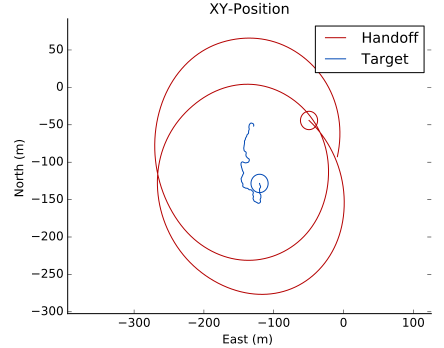
\includegraphics[width=0.7\columnwidth]{figures/orbit_position}
  \caption{Plot of the handoff UAV orbiting the target.}
  \label{fig:orbit_position}
\end{figure}

\begin{figure}[hbt]
  \centering
  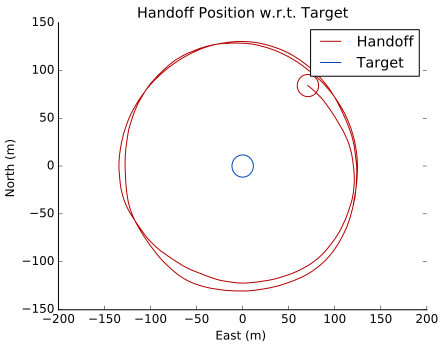
\includegraphics[width=0.7\columnwidth]{figures/orbit_rel_position}
  \caption{Plot of the handoff orbit relative to the target.}
  \label{fig:orbit_rel_position}
\end{figure}

\begin{figure}[hbt]
  \centering
  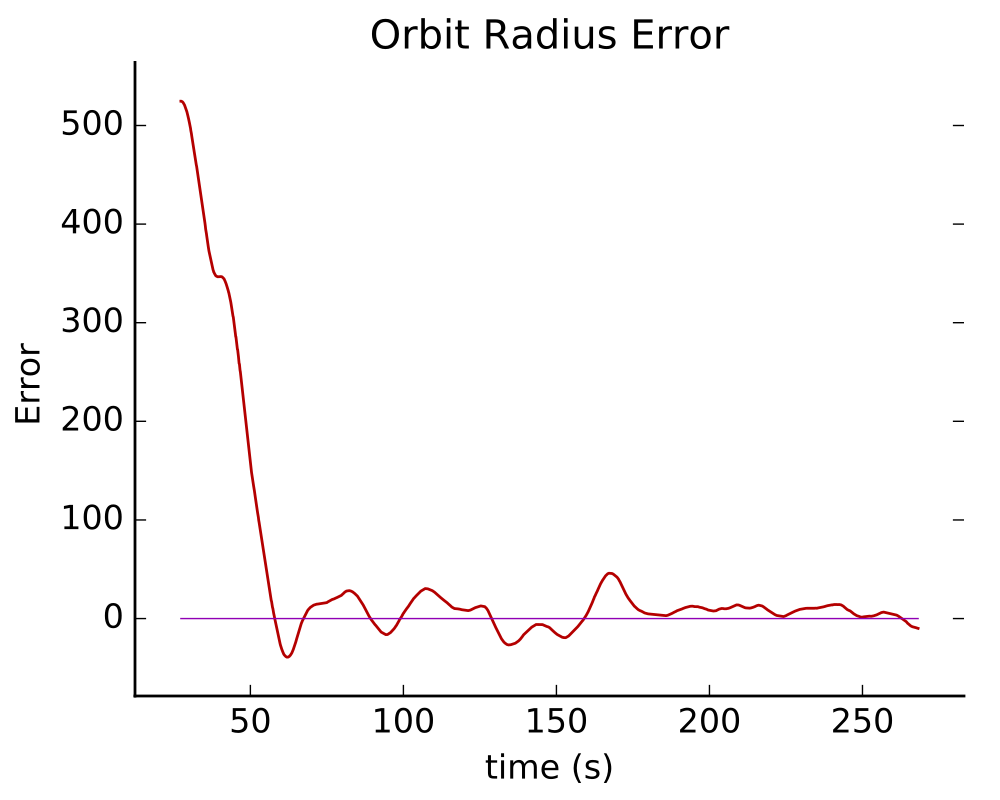
\includegraphics[width=0.7\columnwidth]{figures/orbit_error}
  \caption{Handoff orbit radius error over time.}
  \label{fig:orbit_error}
\end{figure}

% !TEX root=../master.tex
\chapter{Multiple Target Tracking}
\label{ch:target_tracking}

% - new for fixed wing / gimbal

Both the tracking UAV and the Handoff UAV track the ground targets using the R-RANSAC-based visual multiple target tracking (VMTT), originally presented in \cite{NiedfeldtBeard13} and \cite{Ingersoll15}. Although there have been many subsequent publications extending and improving the original algorithm
%% ST: Which references are best to include?
(\cite{DeFranco15}, \cite{IngersollNiedfeldtBeard__},
\cite{IngersollNiedfeldtBeard15}, \cite{NiedfeldtIngersollBeard17}),
this is the first work where the algorithm is used extensively on a fixed-wing aircraft. 
Fixed-wing aircraft operate under different conditions and constraints than multi-rotor aircraft. They must maintain forward velocity with non-holonomic motion constraints, and they often fly at higher altitudes and faster speeds. 
These differences require some unique integration and adaptation of the original algorithm into our particular system. 
This chapter will provide a brief overview of the visual frontend and the R-RANSAC algorithm, along with an explanation of both our implementation and results of using R-RANSAC on a fixed-wing vehicle.

\section{Visual Frontend}
\begin{figure}[hbt]
  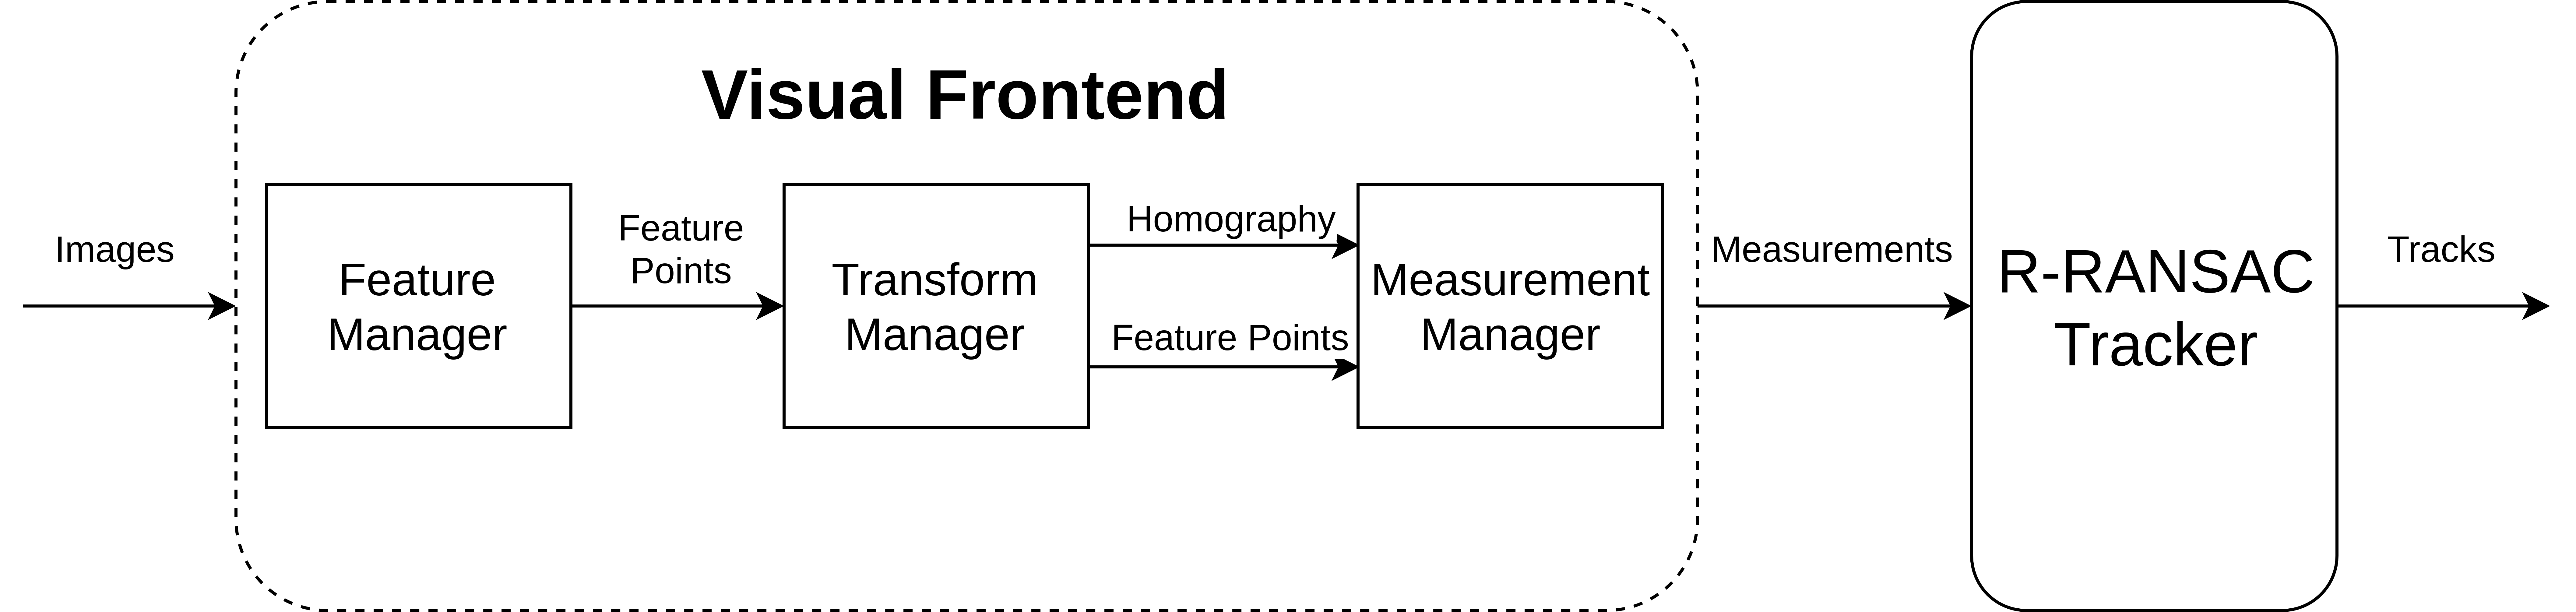
\includegraphics[width=\columnwidth]{figures/vmtt_diagram}
  \caption{Block diagram of visual frontend and R-RANSAC information flow.}
  \label{fig:vmtt_block}
\end{figure}
The visual frontend pipeline is made up of three main blocks--the feature manager, the transform manager, and the measurement manager as seen in Figure~\ref{fig:vmtt_block}. The feature manager receives the current frame as input and finds good features in the image. The features are passed to the transform manager, which estimates the homography between the previous and current frames. The measurement manager uses the image, the features, and the homography to produce meaningful measurements as candidates for new models to track. These measurements are used as input to the R-RANSAC algorithm.

\section{R-RANSAC Tracker}
\subsection{RANSAC Algorithm}
Recursive RANSAC is based upon the original RANSAC (random sample consensus) algorithm, which was first intruduced in \cite{FischlerBolles81}. 
RANSAC is commonly used to fit data to a given model and reject outliers to that model. 
The algorithm uses an iterative process to determine the best model parameters to describe the largest subset of the data possible. 
On each iteration, a subset of the data is randomly sampled containing the minimum number of data points required to represent the model. 
Using the selected points, the appropriate model parameters are computed, and the remaining points are classified as inliers or outliers to the proposed model based on some predetermined error threshold. All points that lie withing the error threshold are referred to as the consensus set. 
If the consensus set has a sufficient number of points, the model parameters are recomputed using all of the points in the consensus set. 
The points outside the consensus set are considered outliers and have no influence on the resulting model. This process is repeated a fixed number of times and the model with the largest consensus set is considered to be the best model and is used as the final solution. 
% Potentially add a linear example 

By way of example, consider that we wanted to use RANSAC to perform linear regression on a set of points. The model would be a straight line and the model parameters could be the slope and y-intercept of the line. The minimum number of points required to define a line is two, so in each iteration of the algorithm, the random sample would consist of two points. Using these two points, we would form a line and determine which points lie within some distance threshold of that line. If the consensus set was sufficiently large, we would consider the line to be a good model for the data and recompute the best fit line using only the points within the consensus set. This process would be repeated for the desired number of iterations, saving the model with the largest consensus set as the best model for the data. Using RANSAC to estimate model parameters in this way has the added advantage of being able to identify and completely reject outliers or exessively noisy datapoints, allowing the model to be more accurate and more representative of the true data.

In the R-RANSAC algorithm, the models are motion models through time. We typically use constant acceleration or constant jerk linear motion models to describe the motion of objects. R-RANSAC uses RANSAC to find and initialize good models, which are then "recursively" propagated through time using a linear filter. RANSAC is then applied to all measurements which do not belong to a model that is currently being tracked to determine if there are good models among the remaining outliers. This allows the R-RANSAC tracker to simultaneously manage an arbitrary number of tracks at any given time.

\section{Adaptations for Fixed-wing vehicles}
\subsection{Two-axis gimbal}
One of the main differences between tracking from a fixed-wing vehicle as opposed to a multirotor, is that the vehicle must remain in constant motion. Accordingly, a gimbal is necessary to maximize the aircraft's ability to maintain a line of sight to the target. We chose to use a two-axis gimbal for this project to allow control of both the azimuth and elevation angles of the camera. The appropriate azimuth and elevation angles are computed according to
\begin{equation}
  \az = \atantwo(\los_y, \los_x)\;,
\end{equation}
and
\begin{equation}
  \el = -\asin(\los_z)\;,
\end{equation}
where $\los$ is the normalized line of sight vector from the UAV to the target in the vehicle body frame.
%% ST: ADD MORE HERE?

\subsection{Parameter Tuning}
Some of the other challenges of implementing the R-RANSAC tracker on a fixed-wing vehicle include higher operating altitudes, faster velocities, and continuously varying viewpoints of the target.
These conditions can make it more difficult for the vehicle to pick up on good, consistent features of the target and can also lead to high variation in the apparent motion of the target.
The apparent motion of the target in the camera frame is minimized when the line of sight to the target and the target's velocity are nearly aligned.
In a constant orbit about a ground target with nearly constant velocity, this alignment happens twice per revolution.
R-RANSAC assumes that targets of interest are moving and therefore uses motion in the image plane to track targets, which makes it more difficult for the tracker to continue tracking the target when the apparent motion is low.

To overcome these challenges, we tuned the algorithm parameters to help the tracker be better suited to having fewer good features and periodically low apparent motion. Table~\ref{tab:vmtt_params} summarizes our parameter choices for the tracking algorithm.

% Please add the following required packages to your document preamble:
% \usepackage[table,xcdraw]{xcolor}
% If you use beamer only pass "xcolor=table" option, i.e. \documentclass[xcolor=table]{beamer}
% Please add the following required packages to your document preamble:
% \usepackage{graphicx}
% \usepackage[table,xcdraw]{xcolor}
% If you use beamer only pass "xcolor=table" option, i.e. \documentclass[xcolor=table]{beamer}
\begin{table}[hbt]
\caption{R-RANSAC Tracking Parameters}
\label{tab:vmtt_params}
\centering
\resizebox{\columnwidth}{!}{%
\begin{tabular}{|>{\centering\arraybackslash}m{0.15\columnwidth}|>{\centering\arraybackslash}m{0.27\columnwidth}|>{\centering\arraybackslash}m{0.09\columnwidth}|>{\centering\arraybackslash}m{0.09\columnwidth}|>{\centering\arraybackslash}m{0.3\columnwidth}|}
\hline
\textbf{Param}                      & \textbf{Description}                                                          & \textbf{Default} & \textbf{Ours} & \textbf{Reasoning}                                                                          \\ \hline
frame stride               & Number of frames between measurements                                                  & 2       & 3         & More frames between measurements equates to more motion.                           \\ \hline
minimum feature velocity   & minimum allowable feature velocity                                                     & 0.002   & 0.0005    & Allows the tracker to detect slower tracks                                         \\ \hline
Nw                         & Window/history size                                                                    & 10      & 25        & A longer window allows the tracker to better determine which tracks are persistent \\ \hline
M                          & Maximum number of models                                                               & 30      & 10        & Allows for fewer good models; less likely to pick up on noise                      \\ \hline
tauR                       & Inlier region threshold                                                                & 0.07    & 0.045     & Better suited for smaller targets                                                  \\ \hline
tau\_CMD                   & consecutive missed detections (CMD) threshold                                          & 4       & 10        & Allows for more missed detections                                                  \\ \hline
tau\_Vmax                  & maximum model speed                                                                    & 0.043   & 0.025     & Allows for slower moving targets                                                   \\ \hline
tau\_T                     & Tracks must have a lifetime counter above this threshold to be considered good tracks. & 4       & 25        & Requires tracks to persist for longer before being considered a good model         \\ \hline
\end{tabular}%
}
\end{table}

\section{Results}
Using the R-RANSAC tracker and a two-axis gimbal setup, we were able to achieve reasonable tracking results for moving ground targets. We tested the tracking algorithm on a fixed-wing aircraft flying approximately 300 meters above a moving vehicle on the ground. With proper tuning, we were able to get the UAV to track the vehicle despite significant jitter in camera feed. Figure~\ref{fig:afrl_tracking} shows a snapshot of tracking the moving ground target.

\begin{figure}[hbt]
  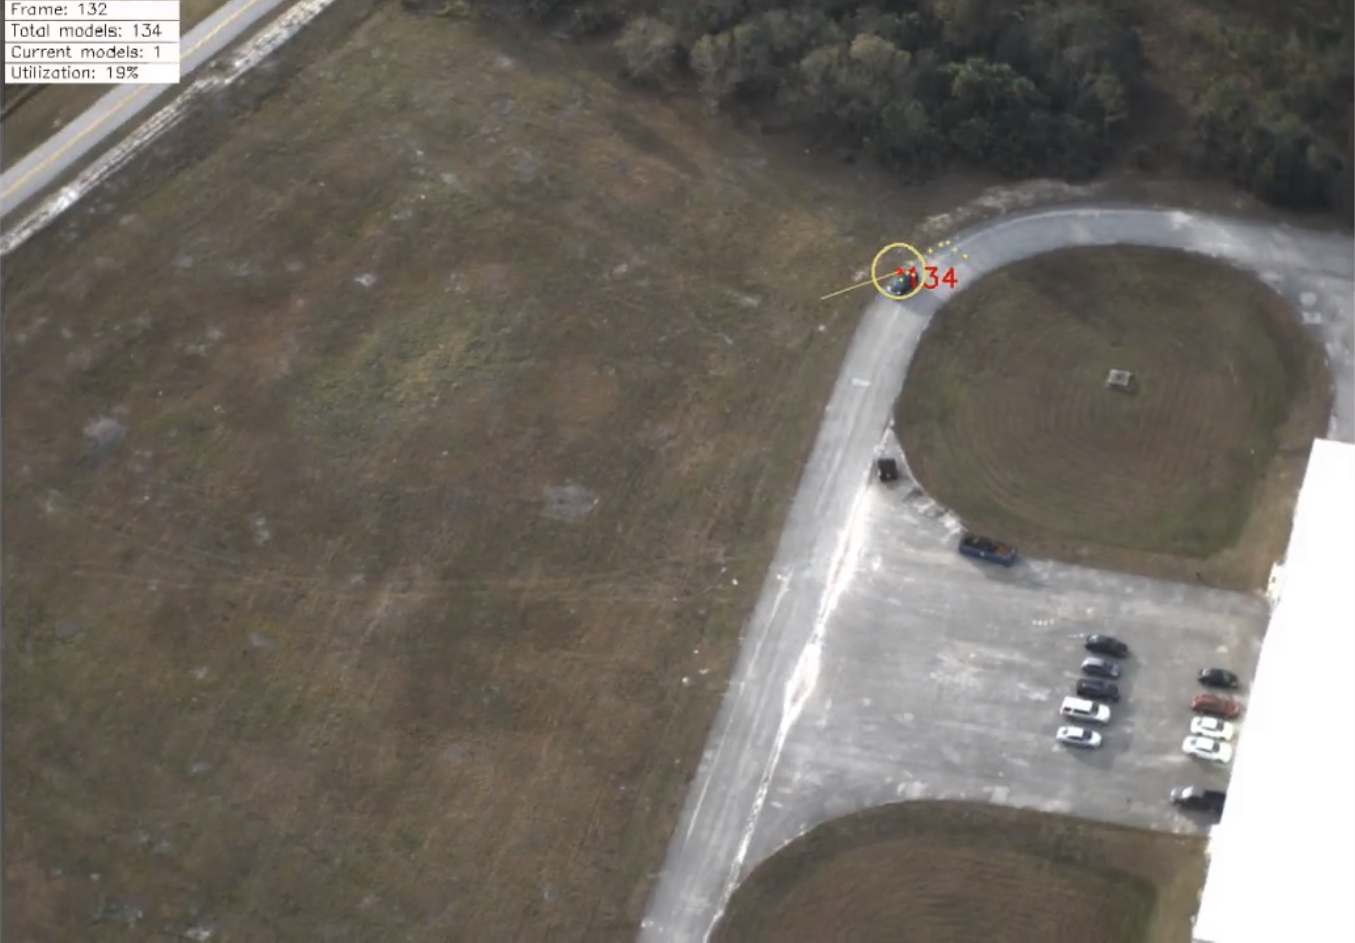
\includegraphics[width=\columnwidth]{figures/afrl_tracking}
  \caption{Snapshot of tracking a moving ground target from a fixed-wing aircraft}
  \label{fig:afrl_tracking}
\end{figure}

% !TEX root=../master.tex
\chapter{Handoff Logic}
\label{ch:handoff_logic}

Once the handoff vehicle is tracking moving objects visually, it must decide which object correlates with the target being tracked by the tracking UAV.
Given a series of observations over time, the handoff UAV should continue tracking the object that is most likely to correspond with the correct target. In order to estimate the correlation between two tracks, the handoff UAV must first align the tracks. For tracks that have a low residual after alignment, the UAV can compare the resulting transformation with the estimated relative pose to see if the two estimates coincide. If a track boths aligns well with the information from the tracking UAV and also coincides with the relative pose estimate, it is considered a good match. This section discusses the method used for track alignment and also the logic used to determine if the a track is a sufficiently good match to complete the handoff.

%  select tracks with low residual after alignment as candidates, and compare the aligment results with the relative pose estimate to see if the two estimates coincide.
% When the handoff UAV finds a track that aligns well with the track from the tracking UAV and also coincides with the relative pose estimate, the handoff UAV can make an informed decision about which object to track persistently. This section discusses the track aligment and the logic used to decide when to officially complete the handoff.

\section{Track Alignment}
Let $\x_k$ represent the tracking UAV's measurement of targets position at the $k$ -th time step and let $\y_{k}$ represent the handoff UAV's measurement of the target at the $k$-th time step. Each measurement is given in the respetive UAV's vehicle-1 frame. We will also define $X$ and $Y$ to be $3 \times n$ matrices, composed of measurements received at the past $n$ timesteps. If we assume that all points in $X$ and $Y$ are in the ground plane, zeroing out the $z$-component, the two sets of measurements will have have a rotational and a translational offset from one another.

We can account for the translation between the two by simply shifting the centroid of each set of measurements to the origin, such that
\begin{equation}
    \bar{X} = X - \frac{1}{n}\sum\limits_{i=1}^{n} \x_i\;,
\end{equation}
and where $\bar{Y}$ is obtained by a similar operation.

Without noise, the relationship between $\bar{X}$ and $\bar{Y}$ would be given by
\begin{equation}
    \bar{Y} = \Rot{\tv}{\hv}\bar{X}\;.
\end{equation}
In the prescence of noise, this equation will not perfectly hold, but we can still estimate the appropriate value for $\Rot{\tv}{\hv}$ by finding the rotation, $R$, such that error is minimized, according to
\begin{equation} \label{eq:Rhat_procrustes}
    \Rothat{\tv}{\hv} = \arg\min\limits_{R}\hspace{0.5em} \norm{R\bar{X} - \bar{Y}}_F\;,
\end{equation}
where $\norm{\cdot}_F$ represents the Frobenius norm.

The solution to Equation~\eqref{eq:Rhat_procrustes} can be found in closed form using singular value decomposition (SVD), according to the result from the orthogonal Procrustes problem \cite{Schonemann1966}.
In our case, we constrain the problem to only include rotation matrices ($\det(R) = 1$), which corresponds with the Kabsch algorithm \cite{Kabsch78}.

First, we compute the cross covariance between $\bar{X}$ and $\bar{Y}$, given by
\begin{equation}
    M = \bar{Y}\bar{X}^\transpose\;.
\end{equation}
Using SVD, $M$ can be decomposed as
\begin{equation}
    M = U\Sigma V^\transpose\;.
\end{equation}
The optimal rotation is given by
\begin{equation} \label{eq:Rhat_svd}
    \Rothat{\tv}{\hv} = U\Sigma' V^\transpose\;,
\end{equation}
where $\Sigma'$ is given by
\begin{equation}
    \Sigma' = \pmat{1 & 0 & 0 \\
                    0 & d & 0 \\
                    0 & 0 & 1}\;,
\end{equation}
where $d$ is the sign $(\pm 1)$ of $\det(UV^\transpose)$. This ensures that the determinant of $\Rothat{\tv}{\hv}$ will be 1. Note that in the original algorithm, $d$ would appear in the bottom row of $\Sigma'$, but because we assume that all points lie in the $xy$-plane, we allow the third row to remain identity and instead place $d$ in the second row.

After computing the optimal value for $\Rothat{\tv}{\hv}$, we can use the remaining residual from Equation~\eqref{eq:Rhat_procrustes} as a measure of how well the two tracks were able to be aligned. We can choose a threshold for the residual, $T_r$, and say that any track which produce a residual less than the threshold is a potential match with the target.

The result of Equation~\eqref{eq:Rhat_svd} will give us the rotation which minimizes the Frobenius norm of the error between the two sets of points, but it is possible that two similarly shaped tracks could produce a low residual, but not be true matches. In order increase our confidence that an object truly does correspond with the target, we can also compare the result of the procrustes analysis with the relative pose estimate between the two vehicles.

For any object which has a residual below the threshold, we also compare the computed rotation, $\Rothat{\tv}{\hv}$, with the rotation estimated by the relative pose estimator, which we will denote as $\Rot[\tilde]{\tv}{\hv}$. We can extract the error between the two rotations according to
\begin{equation}
    e_\theta = \cos^{-1} \left(\e_1^\transpose\Rothat{}{}\Rot[\tilde]{}{\transpose}\e_1\right)\;,
\end{equation}
where $\e_1$ is given by $\pmat{1 & 0 & 0}^\transpose$.

We can derive an estimate of the relative translation between the two UAVs using the sets of points, $\X$ and $\Y$, which can be compared with the relative line of sight estimate to further verify that the tracks truly match. We estimate the relative line of sight according to
\begin{align}
    \p[\hat]_{\TwrtH}^\hv &= \p_{\TwrtTG}^\hv - \p_{\HwrtTG}^\hv \\
        &= \p_{\TGwrtH}^\hv - \Rot{\tv}{\hv}\p_{\TGwrtT}^\tv
\end{align}
where $\Rot{\tv}{\hv}$ is the estimated rotation between the two tracks and $\p_{\TGwrtT}^\tv$ and $\p_{\TGwrtH}^\hv$ represent the most recent measurements in $\X$ and $\Y$ respectively. The translational error is given by
\begin{equation}
    e_t =  \norm{ \p[\hat]_{\TwrtH}^\hv -  \p[\tilde]_{\TwrtH}^\hv }
\end{equation}
where $\p[\tilde]_{\TwrtH}^\hv$ represents the relative line of sight estimate from the relative pose particle filter.

If both the angle and translation errors between the procrustes result and the relative pose estimate are below their respective thresholds, $T_\theta$ and $T_\t$, then we consider the two tracks a match.

When we complete the handoff, the handoff UAV will switch from using the relative pose esimate for estimating the target's position to using the visual LOS. To avoid a discontinuous jump in the LOS input to the orbit control, we introduce a blending parameter, $\gamma_b$, that evolves according to
\begin{equation}
    \gamma_b^+ = \alpha m + (1 - \alpha) \gamma_b\;,
\end{equation}
where $\alpha$ is a tunable parameter that determines the blending transition rate and $m$ is a binary value depending on whether or not the tracks match, given by
\begin{equation}
    m = \begin{cases} 1, & \norm{\Rot[\hat]{\tv}{\hv}\bar{X} - \bar{Y}}_F < T_r, \mbox{ } e_\theta < T_\theta, \mbox{ and } e_t < T_t\\
    0, & \mbox{otherwise}
  \end{cases}\;.
\end{equation}

The blending parameter, $\gamma_b$, can also help to ensure that the handoff only occurs after the errors remain below the desired thresholds for multiple consecutive timesteps. We say that the handoff is officially complete when $\gamma_b$ rises above a threshold, $T_\gamma$, which we set as $0.95$.

% !TEX root=../master.tex
\chapter{Results}
\label{ch:results}


\section{Simulation Setup}
In order to test the full system, we simulated the handoff scenario using Gazebo 7 and ROS. While a hardware demonstration is preferrable, we were able to show a fully working system with simulated noise in software, suggesting that with minor tweaks and tuning, the methods described here would result in a successful hardware implementation.

The aircraft dynamics were simulated according to the framework presented in~\cite{BeardMcLain12}, with parameters for a small fixed-wind UAV. The ground targets are represented by pedestrians that wander randomly within a 140m by 270m area. In order to provide visual features, a satellite image of a rural area is used as the ground plane for the simulated world.

\begin{figure}[hbt]
  \centering
  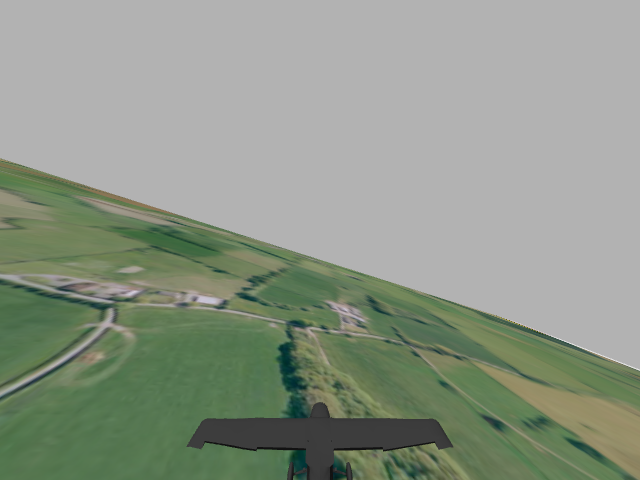
\includegraphics[width=1.0\columnwidth]{figures/sim_chase}
  \caption{Snapshot of the handoff vehicle orbiting about the target above a simulated rural ground plane.}
  \label{fig:sim_chase}
\end{figure}

Each UAV is equipped with IMU and magnetometer sensor plugins and the range sensor used in the relative pose estimator from Chapter~\ref{ch:relative_pose} is simulated by computing the norm of the distance between the two UAVs, with zero-mean Gaussian noise.
Each vehicle also has a camera with a two-axis gimbal.

Becuase the visual from the camera is not directly linked to the targets, it makes it difficult to establish a test to determine with aboslute certainty if the handoff vehicle associates the correct track with the true target.
To overcome this issue, we simulated the camera and tracking information by projecting the positions of the targets into the camera frame of the UAV with noise added to the LOS and camera frame pixel positions.

For simplicity, both UAVs are deployed simultaneously, but the tracking UAV uses absolute position to navigate directly to the target, while the handoff UAV begins estimating the relative pose between aircraft to determine the target's location.
The handoff UAV is able to successfully determine the relative pose between the aircraft and insert into a similar orbit.
As the targets enter the handoff vehicle's field of view, the handoff UAV begins tracking each target and, over time, gains sufficient confidence to complete the handoff.
The handoff vehicle continues to track and orbit the target using only visual information.

\section{Results}
We ran the simulation 500 times and measured the time it took for the handofff vehicle to complete the handoff and whether or not it selected the correct target among 5 different randomly moving targets. We considered it a failure if the UAV couldn't determine the correct target within 15 minutes. The UAV was able to accurately determine the correct target 97.2\% of the time time with an average handoff time of 314 seconds.

We also conducted monte carlo simulations to test the limitations of our approach and to evaluate some of the tradeoffs of certain parameters. The main tradeoff we identified was the time it took the handoff vehicle to make a decision vs. the accuracy of that decision. The handoff logic thresholds and the track comparison window size seemed to be the primary determining factors for this tradeoff. As the requirements for handoff become more difficult to meet, namely lower thresholds and larger window sizes, the accuracy of the handoff increases, but it also takes increasingly long to make a decision. To characterize this tradeoff between the speed of the decision and the accuracy, we varied both the window size and the residual threshold. We ran 100 iterations of each parameter configuration and average the results. Figure~\ref{fig:sim_time_vs_accuracy}-\ref{fig:sim_threshold_vs_time} show the trends observed for various window size and threshold parameters.

\begin{figure}[hbt]
  \centering
  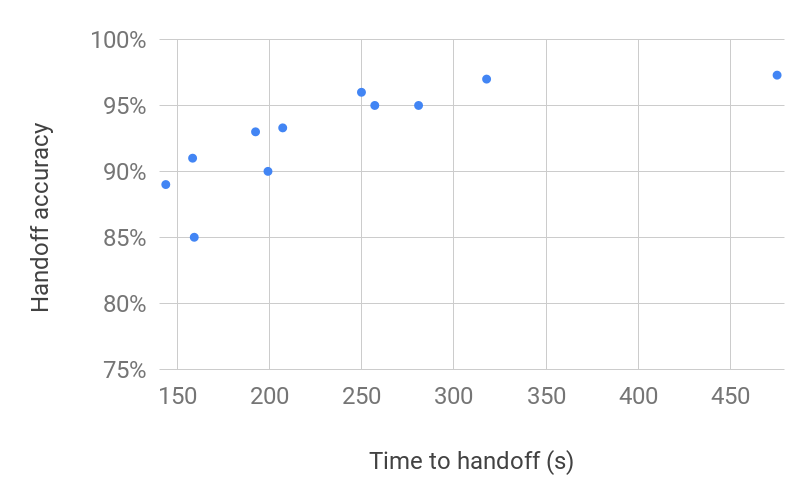
\includegraphics[width=0.7\columnwidth]{figures/sim_time_vs_accuracy}
  \caption{Positive relationship between the time to handoff and handoff accuracy for various window size and threshold values. }
  \label{fig:sim_time_vs_accuracy}
\end{figure}

If the window size was too small or the threshold too high, then the accuracy suffered. The handoff vehicle would make a decision sooner, but it was less likely  to make the correct decision. As the window size increased and the threshold lowered, the conditions for handoff were more stringent and accordingly, accuracy went up. As the accuracy exceeded 97\%, the time it took the handoff vehicle to make a decision increased significantly. Using a window size of 100 and residual threshold of 15 meters seemed to provide a reasonable balance, giving 97.2\% accuracy and a handoff time of 314 seconds, as described above.
\begin{figure}[hbt]
  \centering
  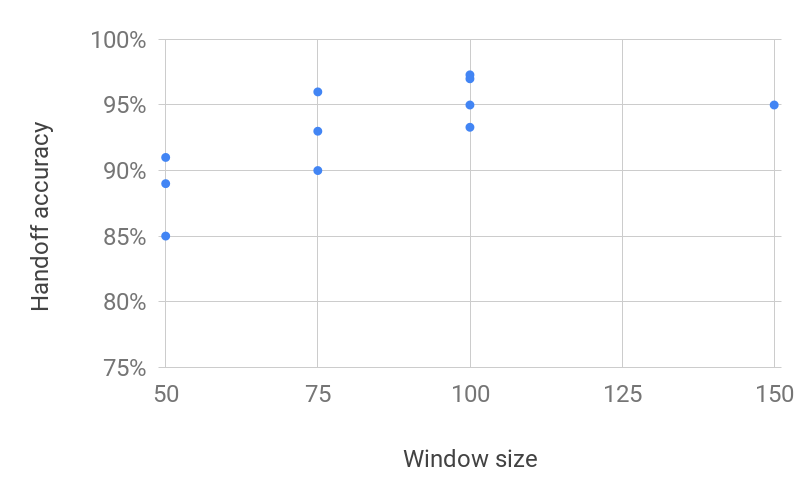
\includegraphics[width=0.7\columnwidth]{figures/sim_window_vs_accuracy}
  \caption{Positive relationship between the handoff logic window size and handoff accuracy for various threshold values.}
  \label{fig:sim_window_vs_accuracy}
\end{figure}

\begin{figure}[hbt]
  \centering
  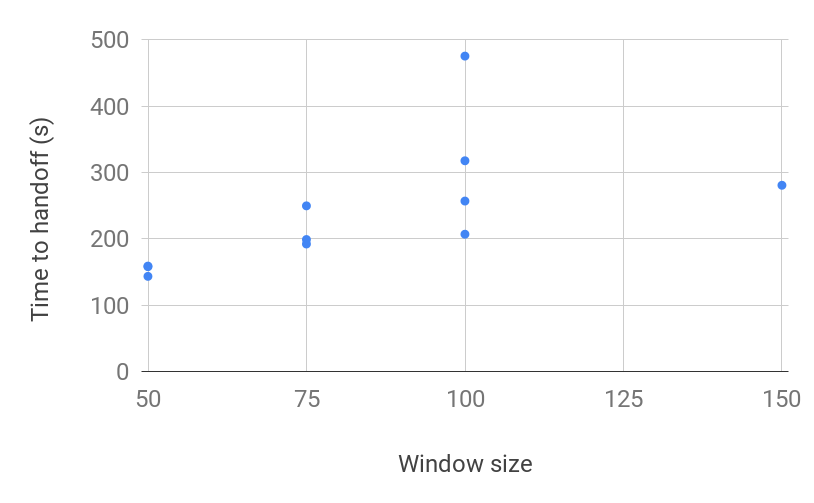
\includegraphics[width=0.7\columnwidth]{figures/sim_window_vs_time}
  \caption{Positive relationship between the handoff logic window size and the time to handoff for various threshold values.}
  \label{fig:sim_window_vs_time}
\end{figure}

\begin{figure}[hbt]
  \centering
  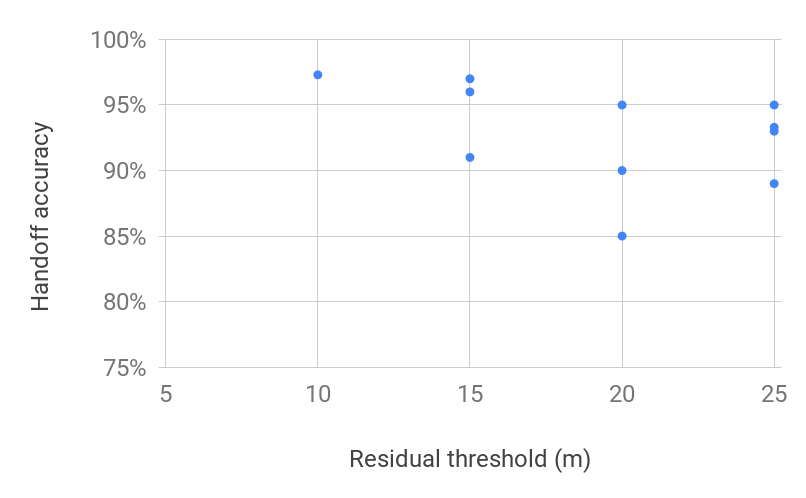
\includegraphics[width=0.7\columnwidth]{figures/sim_threshold_vs_accuracy}
  \caption{Negative relationship between the residual threshold and handoff accuracy for various window size values.}
  \label{fig:sim_threshold_vs_accuracy}
\end{figure}

\begin{figure}[hbt]
  \centering
  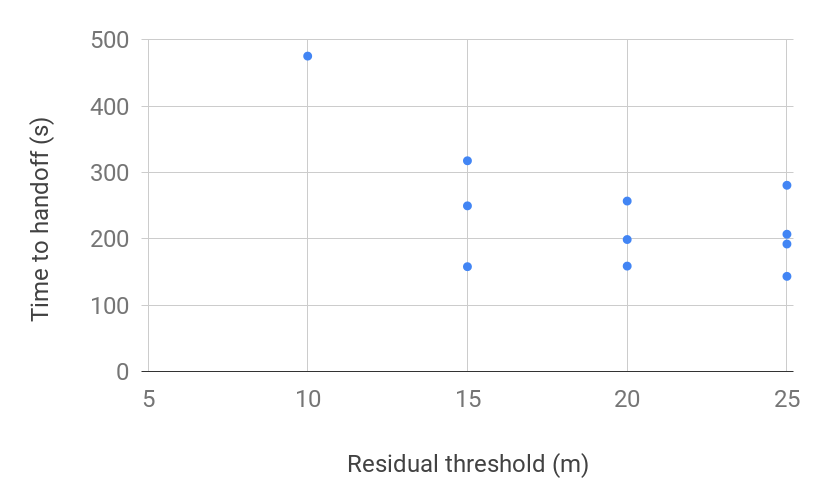
\includegraphics[width=0.7\columnwidth]{figures/sim_threshold_vs_time}
  \caption{Negative relationship between residual threshold and time to handoff for various window size values.}
  \label{fig:sim_threshold_vs_time}
\end{figure}



%We also increased the sensor noise parameters for the simulated range and magnetometer measurements to see how increased noise would affect the performance of the full system. Interestingly, we observed that as we increased the standard deviation of the noise, the performance of the system increased slightly up to a point, then degraded as the noise was increased further, as seen in Figure\stcomment{add plot}. It seems as though a slight increase in the noise

%a slight increase in the noise for both sensors actually improved the performance of the handoff logic, but

% !TEX root=../master.tex
\chapter{Conclusion}
\label{ch:conclusion}


%%%%%%%%%%%%% begin Bibliography %%%%%%%%%%%%%%%%%
\cleardoublepage
\bibliographystyle{IEEEtran}
\bibliography{library} % Use your own BibTex file here

% Include appendix sections here: (or comment these lines out to have no appendices)
\appendix
% % !TEX root=../master.tex
% \appendix{DERIVATIONS} % Do we want this?
\section{Angle of attack dynamics} \label{append:alpha_derivation}
From Equation (2.5-19) in \cite{StevensLewis03} we see that the dynamic equation for $\alpha$ is
\begin{align}
m \dot{\alpha} v_a \cos\beta = -F_T &\sin(\alpha + \alpha_T) - L + mg_3 \\
								&+ mv_a(Q\cos\beta - P_s\sin\beta) \nonumber \;
\end{align}
By solving for $\dot{\alpha}$ and assuming both $\beta$ and $\alpha_T$ are zero, we can simplify the equation to become
\begin{equation}
\dot{\alpha} = \frac{-F_T\sin\alpha - L}{mv_a} + \frac{g_3}{v_a} + Q \;.
\end{equation}
Expanding $g_3$ according to Equation (2.5-17) in \cite{StevensLewis03} gives
\begin{align}
\dot{\alpha} &= \frac{-F_T\sin\alpha - L}{mv_a} \\
&\hspace{2em}+ \frac{g(\sin\alpha\sin\theta + \cos\alpha\cos\phi\cos\theta)}{v_a} + Q \nonumber \;.
\end{align}
where $v_a$ represents airspeed, $F_T$ represents the thrust force, $L$ represents the lift force, $Q$ is the rate of rotation about the body frame y-axis, $g$ is gravity, and $m$ is the airframe mass.

In order to simplify the equations, we will assume that the angles $\alpha, \theta$, and $\phi$ are small and use linear approximations of the sinusoid functions. This provides a linear form of the dynamics given by
\begin{align}
\dot{\alpha} &= \frac{-F_T\alpha - L}{mv_a} + \frac{g\cos(\theta - \alpha)}{v_a} + Q \\
			 &= \frac{-F_T\alpha - L}{mv_a} + \frac{g}{v_a} + Q \;.
\end{align}
We can expand both $F_T$ and $L$ by using the approximations
\begin{equation}
F_T \approx k_{motor}\delta_t^2 - k_T v_a^2 \;
\end{equation}
and
\begin{equation}
L \approx k_L v_a^2
\end{equation}
from \cite{BeardMcLain12},
where $k_{motor}$, $k_T$, and $k_L$ are constants and $\delta_t$ is the throttle control effort.
The resulting dynamic equation is
\begin{equation}
\dot{\alpha} = \frac{-(k_{motor}\delta_t^2 - k_T v_a^2)\alpha - k_L v_a^2}{mv_a} + \frac{g}{v_a} + Q \;.
\end{equation}
Rearranging the terms gives us
\begin{equation} \label{eq:alphadot_rederivation}
\dot{\alpha} = \frac{-(k_{motor}\delta_t^2 - k_T v_a^2)}{mv_a}\alpha + Q - k_L v_a + \frac{g}{v_a} \;.
\end{equation}
Comparing to the linearized dynamic equation used in \cite{Mahony11}, written as
\begin{equation} \label{eq:alphadot_mahony}
\dot{\alpha} = -\frac{c_0}{v_a}\alpha + \dot{\theta} + \alpha_0 \;,
\end{equation}
the form is very similar, differing only in that the dynamic equation in \eqref{eq:alphadot_rederivation} replaces the constants $c_0$ and $\alpha_0$ with functions of $v_a$.

Accordingly, defining
\begin{equation} \label{eq:c0_Va_append}
c_0(v_a) = \frac{k_\delta - k_T v_a^2}{m}
\end{equation}
and
\begin{equation}
\alpha_0(v_a) = \frac{g}{v_a} - \frac{k_L}{m}v_a \;,
\end{equation}
we can rewrite \eqref{eq:alphadot_rederivation} in the form of \eqref{eq:alphadot_mahony} as
\begin{equation} \label{eq:alphadot_final}
\dot{\alpha} = -\frac{c_0(v_a)}{v_a}\alpha + \dot{\theta} + \alpha_0(v_a) \;.
\end{equation}
Note that in \eqref{eq:c0_Va_append} we assume that we don't have knowledge of the value of $\delta_t$ and accordingly replaced $k_{motor}\delta_t^2$ with a constant $k_\delta$.

For flights where the airspeed is held near constant, there is little performance advantage of using one dynamic derivation over the other, but the dynamic equation given in \eqref{eq:alphadot_final} does track the angle of attack better over varying airspeeds.

\subsection{Error State Dynamics}
\label{append:error_dyn_derivation}
Because we define the gyro bias dynamics in \eqref{eq:gbias_dynamics} to be zero, the error state dynamics will simply be represented by the state estimate noise, $\noise_{\gbias}$, giving us
\begin{equation*}
  \dgbias[\dot] = \noise_{\gbias} \;.
\end{equation*}

For the angle of attack, we will follow Equation \eqref{eq:dxdot_error} to arrive at the error state dynamics. Expanding all terms required to compute $\bar{\f}$, we get
\begin{align}
  \dot{\dalpha} &= -\frac{c_0(v_a)}{v_a}\alpha + \dot{\theta} + \alpha_0(v_a) \\
    &= \bigg(\frac{-(k_\delta - k_T (v_a + \noiseu_{v_a})^2)}{m(v_a + \noiseu_{v_a})}(\hat{\alpha} + \dalpha) \nonumber \\
    &\hspace{2em}+ (\angvel[\tilde] - \gbias[\hat] - \dgbias - \noiseu_{\angvel})\cdot\vect{e}_2 \nonumber \\
    &\hspace{2em}- k_L (v_a + \noiseu_{v_a}) + \frac{g}{(v_a + \noiseu_{v_a})}\bigg) \\
    &\hspace{1em}- \bigg(\frac{-(k_\delta - k_T v_a^2)}{mv_a}\hat{\alpha} + (\angvel[\tilde] - \gbias[\hat])\cdot\vect{e}_2 \nonumber \\
    &\hspace{2em}- k_L v_a + \frac{g}{v_a }\bigg) \nonumber \;.
\end{align}
Assuming $\noiseu_{v_a} \ll v_a$, we can simplify the equation to
\begin{align}
  \dot{\dalpha} &= \bigg(\frac{-(k_\delta - k_T v_a^2)}{mv_a}(\hat{\alpha} + \dalpha) \\
    &\hspace{2em}+ (\angvel[\tilde] - \gbias[\hat] - \dgbias - \noiseu_{\angvel})\cdot\vect{e}_2 \\
    &\hspace{2em}- k_L v_a + \frac{g}{v_a}\bigg) \\
    &\hspace{1em}- \bigg(\frac{-(k_\delta - k_T v_a^2)}{mv_a}\hat{\alpha} + (\angvel[\tilde] - \gbias[\hat])\cdot\vect{e}_2 \\
    &\hspace{2em}- k_L v_a + \frac{g}{v_a }\bigg) \\
    &= \frac{-(k_\delta - k_T v_a^2)}{mv_a}\dalpha - (\dgbias + \noiseu_{\angvel})\cdot\vect{e}_2 \;,
\end{align}
giving us the dynamic equation for the angle of attack error state.

% !TEX root=../master.tex

\chapter{Learning-based Object Re-identification}

\section{Background and Motivation}
One of the challenging aspects of performing a moving target handoff is ensuring, with enough confidence, that the handoff UAV has successfully identified the correct target before allowing the tracking UAV to leave.
In our current implementation, we only use classical feature tracking methods to determine the motion of the target and compare it with objects observed by the handoff vehicle.
Although we use vision-based features to track the target, we do not directly use visual information about the target as a descriptor to be used in comparing with other moving objects.
In the past few there have been increasingly impressive results in visual object classification and identification using deep neural networks (DNNs).
We conducted a preliminary study to see if we could utilize a deep neural network to encode and compare visual information about the target visually to objects observed by the handoff UAV. This appendix discusses the network architecture and training methods used, as well as some preliminary, but promising results.

\section{Implementation}
In order to demonstrate feasibility, we limited the scope of our study to focus specifically on person re-identification. There are many proposed methods for person re-identification. Many use only visual information \cite{} while some use recurrent networks to encode temporal information as well \cite{}.
We decided to base our architecture and methodology on the work done by Wang et al. in \cite{Wang2018} to create and train a network with a DenseNet architecture \cite{DenseNet}. The model is trained to take cropped bounding box images of people and embed them into clusters within a 128-dimensional vector space. The goal is to train the network in such a way that the cluster associated with each person is distinct and well-distanced (in an L2 norm sense) from embedded clusters of other people. This allows us to compare or identify people simply by measuring their L2 distance in the embedded vector space. Although we focused specifically on people for this study, we believe the extension to other classes of objects would be fairly straightforward, given sufficient data.

We trained the network using the Market-1501 dataset \cite{Market1501}, which consists of multiple cameras, allowing for multiple varied shots of the same people. Originally, we used the triplet loss function given in \cite{Wang2018}. The loss function is computed over a batch of $P$ people with $K$ unique images each. All images are embedded using the neural network and then their L2 distances are compared. For each image, the closest negative (non-matching embedding) and the furthest positive (matching embedding) are found and used to compute the total loss function, given by
\begin{equation}
    \ell = \sum_{p=1}^P \sum_{k=1}^K
            \ln \Bigg(1 + \exp\bigg(\big(
                m + (\text{closest positive})
                  - (\text{furthest negative})
            \big)\bigg)\Bigg)\;,
\end{equation}
where
\begin{equation}
    \text{closest positive} = \max_{a=1,\dots,K}D\left( \phi(x_p^k), \phi(x_p^a)\right);,
\end{equation}
\begin{equation}
    \text{furthest negative} = \min_{\substack{q=1,\dots,P \\ b=1,\dots,K \\ q\neq p}}
                                D\left( \phi(x_p^k), \phi(x_q^b)\right)\;,
\end{equation}
and $m$ represents a desired margin of separation between clusters.

Training using this loss function would decrease the total loss fairly well, but the network seemed to find a local minimum where it could minimize the loss simply by driving all embeddings toward the origin. In an effort to mitigate this challenge, we modified the loss function to minimize the ratio between the furthest positive and the closest negative. Accordingly, the loss function became
\begin{equation}
\label{eq:ratio_loss1}
    \ell = \sum_{p=1}^P \sum_{k=1}^K
            \frac{\text{furthest positive} + m}{\text{closest negative}} \;.
\end{equation}

Using this ratio-based loss removed any incentive to drive the embeddings toward the origin, but instead, allowed the network to spread out the clusters freely. Training with this loss had the advantage that we were able to train the network for longer without producing a degenerate solution and accordingly, the network learned how to more accurately represent detailed information. It was also quite a bit faster than the original loss function, providing a speed increase of about 20\%.

The main disadvantage to using this loss function is that it made the distances between an image and it's closest positive inconsistent across different people. This property is undesirable because it makes it difficult to infer whether or not two images match purely based on the L2 distance. Some matching images would be spaced 1 unit apart and others would be spaced 15-20 units apart.

In order to overcome this challenge, we reformed the loss function again to include a term that would penalize large distances between positive examples. The loss function became
\begin{equation}
\label{eq:ratio_loss2}
    \ell = \sum_{p=1}^P \sum_{k=1}^K
            \frac{\text{furthest positive} + m}{\text{closest negative}} + k(\text{furthest positive})\;,
\end{equation}
where $k$ is a scaling constant. We used a value of 0.1 for $k$.

We continued to train the previously trained network using this new loss function, hoping that it would maintain its understanding of how to group unique identities, but also learn to condense those embeddings to minimize the distance between positive examples. In general, the distances did decrease and the variability in distances within clusters was reduced, although not totally eliminated. Determining an effective way to allow the network to spread clusters out freely in a more consistent manner is a topic for future research and development.


\section{Results}

We trained the first ratio loss function given in Equation \eqref{eq:ratio_loss1} for about 13,000 iterations after which we switched to the second ratio loss given in \eqref{eq:ratio_loss2}. We continued training for another 5000 iterations and were able to obtain fairly good results. The network was able to maintain the accuracy that had been learned by the initial loss function, but also learned to embed positive examples closer together, bringing the max distance down from about 20 to 5.

In order to evaluate the progress of the network, we used a qaulitative measure of accuracy. Periodically, we sampled a batch of 20 people, each with 5 images, from the test dataset. We then calculated the embeddings of each image and the distances between all images. We randomly selected an image and displayed the 5 nearest images and their distances. Ideally, we would expect the chosen image and its 4 nearest embeddings to have the same identity and the 5th to be another person with a distance at least the desired margin further than the furthest positive example. Below we give some qaulitative results and our observations regarding the network's performance.

The network was usually fairly confident at re-identifying people with bright colors or distinct patterns such as in Figures 1-4.
\begin{figure}[H]
\label{fig:bright1}
        \centering 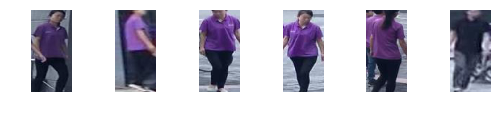
\includegraphics[width=0.8\columnwidth]{figures/person_reid/example7_confident.png}
        \caption{Example of bright clothing.}
\end{figure}

\begin{figure}[H]
\label{fig:bright2}
    \centering 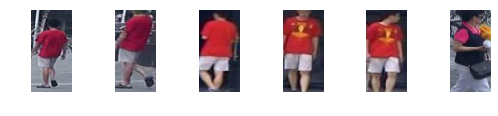
\includegraphics[width=0.8\columnwidth]{figures/person_reid/example8_confident.png}
    \caption{Another example of bright clothing.}
\end{figure}

\begin{figure}[H]
\label{fig:pattern1}
    \centering 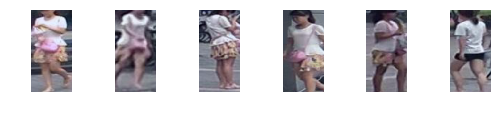
\includegraphics[width=0.8\columnwidth]{figures/person_reid/example4_perfect.png}
    \caption{Example of unique patterned clothing.}
\end{figure}

\begin{figure}[H]
\label{fig:pattern2}
    \centering 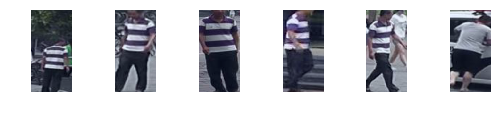
\includegraphics[width=0.8\columnwidth]{figures/person_reid/example12_pattern.png}
    \caption{Another example of patterned clothing.}
\end{figure}

It also performed surprisingly well in some difficult situations, such as when two people are similarly dressed, when the lighting varied between cameras, or when the same person is seen in multiple contexts (Figures 5-8).

\begin{figure}[H]
    \centering 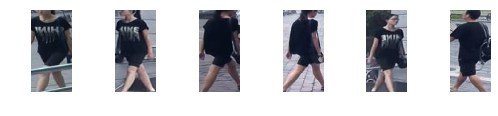
\includegraphics[width=0.8\columnwidth]{figures/person_reid/example11_accurate_despite_similarities.png}
    \caption{Successful classification despite there being two similarly dressed people.}
\end{figure}

\begin{figure}[H]
    \centering 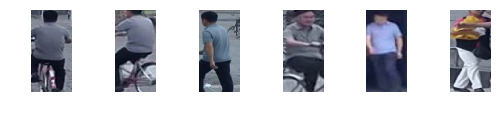
\includegraphics[width=0.8\columnwidth]{figures/person_reid/example8_different_context.png}
    \caption{Successful classification in varied lighting.}
\end{figure}

\begin{figure}[H]
    \centering 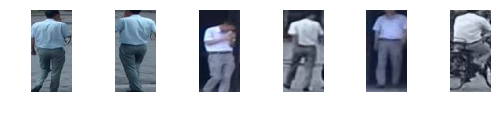
\includegraphics[width=0.8\columnwidth]{figures/person_reid/example2_lighting.png}
    \caption{Another example of successful classification in varied lighting.}
\end{figure}

\begin{figure}[H]
    \centering 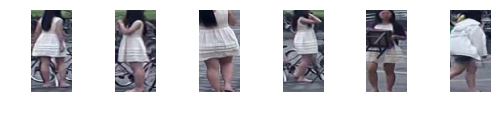
\includegraphics[width=0.8\columnwidth]{figures/person_reid/example6_different_context.png}
    \caption{Successful classification in varied contexts (the woman is carrying furniture and wearing a cardigan in the 5th image).}
\end{figure}

Often, even the failure cases were reasonable, such as two people that had similar clothing, scenes with common prominent features, or specific viewpoints that made classification difficult (Figures 9-12).

\begin{figure}[H]
    \centering 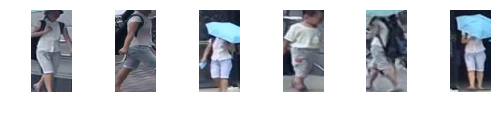
\includegraphics[width=0.8\columnwidth]{figures/person_reid/example1_similar.png}
    \caption{Incorrect classification of 4th image - similar clothing.}
\end{figure}

\begin{figure}[H]
    \centering 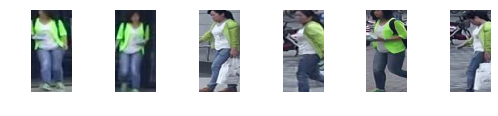
\includegraphics[width=0.8\columnwidth]{figures/person_reid/example3_similar.png}
    \caption{Incorrect classification of 3rd and 4th images - similar clothing.}
\end{figure}

\begin{figure}[H]
    \centering 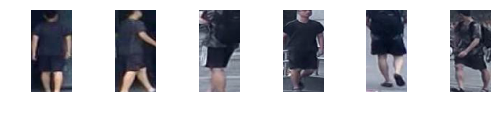
\includegraphics[width=0.8\columnwidth]{figures/person_reid/example5_reasonable_mistake.png}
    \caption{Incorrect classification of 3rd, 5th, and 6th images - similar clothing.}
\end{figure}

\begin{figure}[H]
    \centering 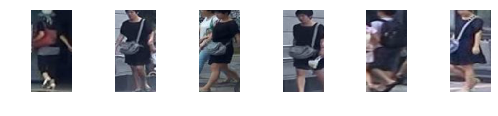
\includegraphics[width=0.8\columnwidth]{figures/person_reid/example9_no_matches.png}
    \caption{Incorrect classification of all images - grey undershirt mistaken as grey handbag.}
\end{figure}

Interestingly enough, it even seemed as though the network has some form of a bike detector, as seen in the failure mode of Figure 13.

\begin{figure}[H]
    \centering 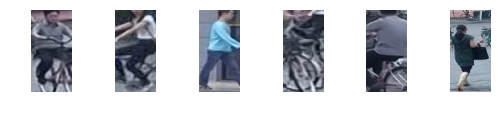
\includegraphics[width=0.8\columnwidth]{figures/person_reid/example10_bike_detector.png}
    \caption{Incorrect classification of 2nd, 3rd, 4th, and 6th images - seems to have been looking for bikes, at least partially.}
\end{figure}


\section{Conclusions}
With more training and some improvements in the loss function, we propose that using this or a similar method of training a neural network could prove useful in classifying and re-identifying objects based on visual information. Such a network would be especially useful in the case of the moving target handoff problem where the tracking vehicle could simply send the 128-dimensional embedding of the target object, allowing the handoff vehicle to compare the L2 embedding distance between the target and moving objects in its field of view. Not only does this provide a means of comparing valuable visual information, but it can also be done without needing to directly pass large image files between the vehicles. With some improvemens and increased reliability, this would provide a useful tool to take advantage of rich visual information that is currently not being utilized in our moving target handoff solution.

% % !TEX root=../master.tex

\end{document}
